\documentclass[11pt,openany]{book}
\raggedbottom

% Load packages
\usepackage[utf8]{inputenc} % for unicode input
\usepackage{microtype}
\usepackage{bm}
\usepackage{enumitem}
\usepackage{geometry} % for page layout
\usepackage{hyperref} % for hyperlinks
\usepackage{tocbibind} % includes the bibliography in the table of contents
\usepackage{amsmath, amsfonts, amssymb, amsthm} % for advanced math formatting
\usepackage{lipsum} % generates filler text
\usepackage{fancyhdr}
\usepackage[table]{xcolor} % for cell coloring
\usepackage{graphicx} % for including images
\usepackage{booktabs} % for professional looking tables
\usepackage[normalem]{ulem} % for underlining
\usepackage[document]{ragged2e} % for text alignment
\usepackage{tikz} % for drawing
\usepackage{algorithm}
\usepackage{algpseudocode}
\usepackage{wrapfig}
\usepackage{circuitikz}
\usepackage{caption}
\usepackage{venndiagram}
\usepackage{multicol}
\usepackage{listings}
\usepackage{adjustbox}
\usepackage{multirow}


% TikZ libraries
\usetikzlibrary{circuits.logic.US, arrows.meta, positioning, calc, fit, decorations.markings, math}

% Document geometry (page size, margins)
\geometry{a4paper, left=20mm, right=20mm, top=25mm, bottom=30mm}

% Custom page style for centered page numbers
\pagestyle{fancy}
\fancyhf{} % Clear all header and footer fields
\fancyhead[RE]{\leftmark} % Left Even pages - Chapter number and name
\fancyhead[RO]{Notes by Ali EL AZDI} % Right Odd pages - Custom message
\fancyfoot[CE,CO]{\thepage} % Centered page number in the footer for both even and odd pages
\renewcommand{\headrulewidth}{0pt}
\renewcommand{\footrulewidth}{0pt}

% Custom commands
\newcommand*\xor{\oplus}
\newcommand{\minidash}{\text{-}}

% Custom spacing command
\makeatletter
\newcommand{\vspacer}[1]{%
  \ifvmode
    \vskip#1\relax
  \else
    \@bsphack
    \vadjust{\vskip#1\relax}
    \@esphack
  \fi
}
\makeatother

%%%%%%%%%%%%%%%%%%% Verilog CODE STYLING %%%%%%%%%%%%%%%%%%%%%%%%%%%%%
\definecolor{keywordcolor}{rgb}{0.5,0.0,0.33}
\definecolor{backgroundcolor}{rgb}{0.95,0.95,1.0}
\definecolor{commentcolor}{rgb}{0.129,0.384,0.529}
\definecolor{stringcolor}{rgb}{0.16,0.00,1.00}
\definecolor{rulecolor}{rgb}{0.46,0.43,0.5}
\definecolor{codegray}{rgb}{0.5,0.5,0.5}

\lstdefinestyle{verilogstyle}{
  language=Verilog,
  basicstyle=\ttfamily\footnotesize,
  backgroundcolor=\color{backgroundcolor},
  commentstyle=\color{commentcolor}\ttfamily, % Add \ttfamily to ensure comments are in typewriter font
  morecomment=[l][\color{commentcolor}\ttfamily]{//}, % Line comment in Verilog
  morecomment=[s][\color{commentcolor}\ttfamily]{/*}{*/}, % Block comments in Verilog
  morekeywords={module, input, output, wire, endmodule, endcase, default, tri, assign, always, if, else, begin, end, case, endcase, parameter}, % Add Verilog keywords
  keywordstyle=\color{keywordcolor},
  stringstyle=\color{stringcolor},
  showstringspaces=false,
  frame=single,
  rulecolor=\color{rulecolor}, % Frame color
  breaklines=true,
  numbers=left,
  numberstyle=\tiny\color{codegray},
  tabsize=2
}

\lstnewenvironment{verilog}
  {\lstset{style=verilogstyle}}
  {}

%%%%%%%%%%%%%%%%%%% C CODE STYLING %%%%%%%%%%%%%%%%%%%%%%%%%%%%%
\definecolor{ckeywordcolor}{rgb}{0.8,0.1,0.1}
\definecolor{cbackgroundcolor}{rgb}{0.95,0.95,0.95}
\definecolor{ccommentcolor}{rgb}{0.0,0.5,0.0}
\definecolor{cstringcolor}{rgb}{0.1,0.1,0.8}
\definecolor{crulecolor}{rgb}{0.5,0.5,0.5}
\definecolor{ccodegray}{rgb}{0.6,0.6,0.6}

\lstdefinestyle{cstyle}{
  language=C,
  basicstyle=\ttfamily\footnotesize,
  backgroundcolor=\color{cbackgroundcolor},
  commentstyle=\color{ccommentcolor}\ttfamily,
  keywordstyle=\color{ckeywordcolor},
  stringstyle=\color{cstringcolor},
  showstringspaces=false,
  frame=single,
  rulecolor=\color{crulecolor},
  breaklines=true,
  numbers=left,
  numberstyle=\tiny\color{ccodegray},
  tabsize=2
}

\lstnewenvironment{cc}
  {\lstset{style=cstyle}}
  {}

%%%%%%%%%%%%%%%%%%% Assembly CODE STYLING %%%%%%%%%%%%%%%%%%%%%%%%%%%%%
\definecolor{akeywordcolor}{rgb}{0.0, 0.2, 0.4}
\definecolor{abackgroundcolor}{rgb}{0.98, 0.99, 1.0}
\definecolor{acommentcolor}{rgb}{0.0, 0.4, 0.6}
\definecolor{astringcolor}{rgb}{0.2, 0.4, 0.8}
\definecolor{arulecolor}{rgb}{0.6, 0.7, 0.8}
\definecolor{acodegray}{rgb}{0.3, 0.4, 0.5}

\lstdefinestyle{assembly}{
  language=[x86masm]Assembler,
  basicstyle=\ttfamily\footnotesize,
  backgroundcolor=\color{abackgroundcolor},
  commentstyle=\color{acommentcolor}\ttfamily,
  keywordstyle=\color{akeywordcolor},
  stringstyle=\color{astringcolor},
  showstringspaces=false,
  frame=single,
  rulecolor=\color{arulecolor},
  breaklines=true,
  numbers=left,
  numberstyle=\tiny\color{acodegray},
  tabsize=2,
  morekeywords={li, and, add, addi, srli, bne}
}

\lstnewenvironment{assembly}
  {\lstset{style=assembly}}
  {}

%%%%%%%%%%%%%%%%%%%%%%%%%%%%%%%%%%%%%%%%%%%%%%%%%%%%%%%%
%%%%%%%%%%%%%%%%%%% JAVA CODE STYLING %%%%%%%%%%%%%%%%%%%%%%%%%%%%%
\definecolor{javakeywordcolor}{rgb}{0.0, 0.0, 0.5}
\definecolor{javabackgroundcolor}{rgb}{0.95, 0.95, 0.95}
\definecolor{javacommentcolor}{rgb}{0.0, 0.5, 0.0}
\definecolor{javastringcolor}{rgb}{0.6, 0.0, 0.0}
\definecolor{javarulecolor}{rgb}{0.5, 0.5, 0.5}
\definecolor{javagray}{rgb}{0.6, 0.6, 0.6}

\lstdefinestyle{javastyle}{
  language=Java,
  basicstyle=\ttfamily\footnotesize,
  backgroundcolor=\color{javabackgroundcolor},
  commentstyle=\color{javacommentcolor}\ttfamily,
  keywordstyle=\color{javakeywordcolor},
  stringstyle=\color{javastringcolor},
  showstringspaces=false,
  frame=single,
  rulecolor=\color{javarulecolor},
  breaklines=true,
  numbers=left,
  numberstyle=\tiny\color{javagray},
  tabsize=2,
  morekeywords={class, public, private, protected, extends, implements, interface, import, package, new, return, void, static}
}

\lstnewenvironment{java}
  {\lstset{style=javastyle}}
  {}

%%%%%%%%%%%%%%%%%%%%%%%%%%%%%%%%%%%%%%%%%%%%%%%%%%%%%%%%
% Document begins
\begin{document}


% Title Page
\begin{titlepage}
    \centering
    \vspace*{1cm}
    \Huge
    Computer Architecture \newline
    \vspace{10px}
    \LARGE IN BA3 - Paolo IENNE
    \vspace*{10px}
    \newline
    \Large Notes by Ali EL AZDI

    \vfill
    \large
    September 11, 2024
\end{titlepage}

\begin{center}
    \vspace*{1cm}
    \textbf{Introduction}
    \newline
    \paragraph[short]{}{This document is designed to offer a LaTeX-styled overview of the Computer Architecture course, emphasizing brevity and clarity. Should there be any inaccuracies or areas for improvement, please reach out at ali.elazdi@epfl.ch for corrections. For the latest version, check my GitHub repository.}
    \newline
   \url{
        https://github.com/elazdi-al/comparch/blob/main/main.pdf
    }
    \newline
\end{center}

% Table of Contents
\tableofcontents

 % Including chapter0.tex from chapters folder
\chapter{Part I(a) - ISA Reminder, Assembly Language, Compiler - W 1.1}
\textbf{hum...welcome back} \newline
\textit{In the first part of the course, professor introduced (for motivational purposes) how computer architecture, specifically processors, have become essential to our lives, and how the field is growing exponentially. (didn't think it was essential to mention here...)}

\section{From High Level Languages to Assembly Language}
\subsection{High Level Languages}
\textit{When talking about programming we usually think of programs that look like this\dots} \newline \vspace*{5px}

\begin{minipage}[htp]{0.4\textwidth} % Use \textwidth to ensure it spans the page width
\begin{cc}
int data = 0x00123456;
int result = 0;
int mask = 1;
int count = 0;
int temp = 0;
int limit = 32;
do {
    temp = data & mask;
    result = result + temp;
    data = data >> 1;
    count = count + 1;
} while (count != limit);
\end{cc}
\end{minipage}
\hfill
\vline
\hfill
\begin{minipage}[htp]{0.4\textwidth}
    \centering
    \begin{tabular}{|c|c|}
        \hline
        \textbf{name} & \textbf{value} \\ \hline
        data       & 0x00123456  \\ \hline
        result     & 0           \\ \hline
        mask       & 1           \\ \hline
        count      & \dots       \\ \hline
        temp       &             \\ \hline
        limit      &             \\ \hline
        \dots      &             \\ \hline
        my\_float  & 3.141529    \\ \hline
        a\_string  & Hello world! \\ \hline
        \end{tabular}
\end{minipage}

\subsection{Assembly Language}
We use this code because it enables us to build a \textit{Finite State Machine}, which isn't feasible with C code. This language provides a more rigid format with a sequence of numbered instructions, an \textit{opcode}, predefined variable names, and the ability to \textbf{jump between lines}.
\newpage
\begin{center}
    \begin{assembly}
    li x1, 0x00123456
    li x2, 0
    li x3, 1
    li x4, 0
    li x5, 0
    li x6, 32
loop: and x5, x1, x3
    add x2, x2, x5
    srli x1, x1, 1
    addi x4, x4, 1
    bne x4, x6, loop
    \end{assembly}
\end{center}

\section{Processors}
\textbf{Remember, a processor can be decomposed into five components:} \newline
\begin{itemize}[noitemsep]
    \item[-] \textbf{ALU (Arithmetic and Logic Unit)}: Performs arithmetic and logical operations.
    \item[-] \textbf{Register File}: Stores data temporarily for quick access during processing.
    \item[-] \textbf{Memory}: Holds data and instructions needed by the processor.
    \item[-] \textbf{Control Logic}: Directs the operation of the processor by coordinating the other components.
    \item[-] \textbf{PC (Program Counter)}: Keeps track of the address of the next instruction to be executed.
    \item[-] \textbf{Instruction Memory}: Stores the program instructions that the processor will execute.
\end{itemize}
\begin{center}
    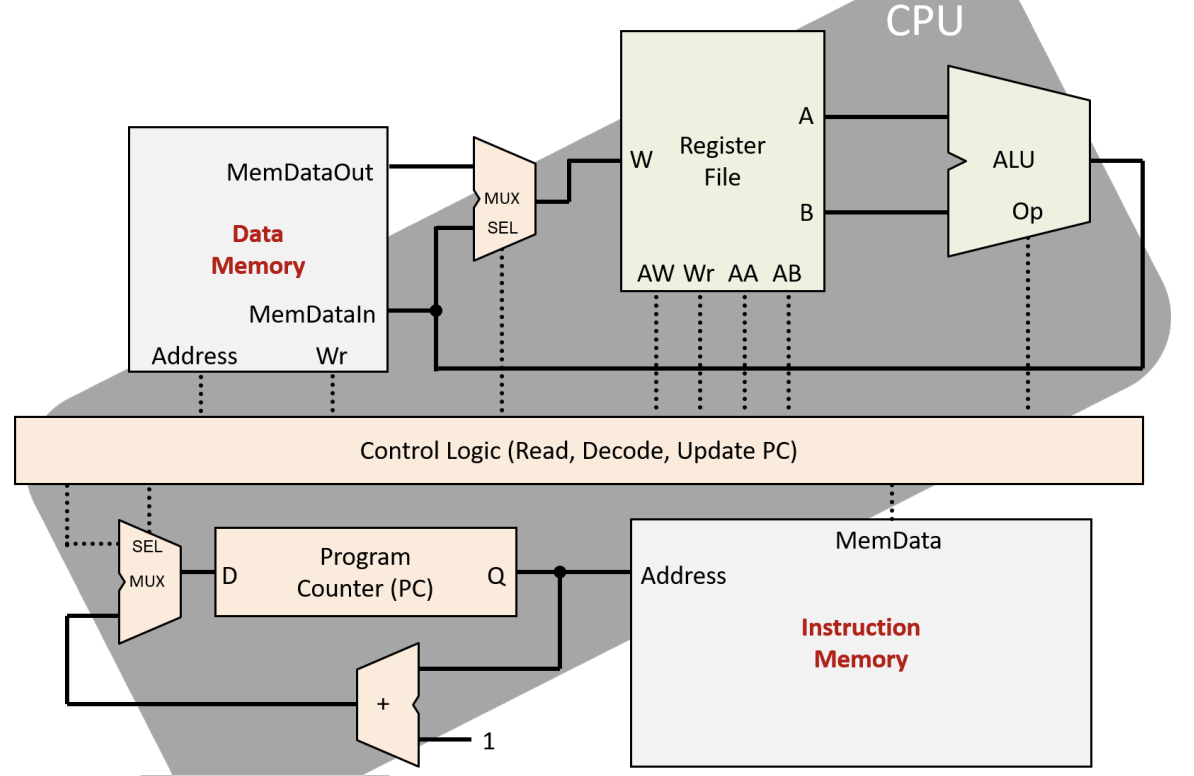
\includegraphics[width=0.5\textwidth]{chapters/chapter1a/images/processor.png}
\end{center}

We may distinguish three types of general operations made by the processor: \newline
\subsubsection*{Encoding}
\begin{center}
    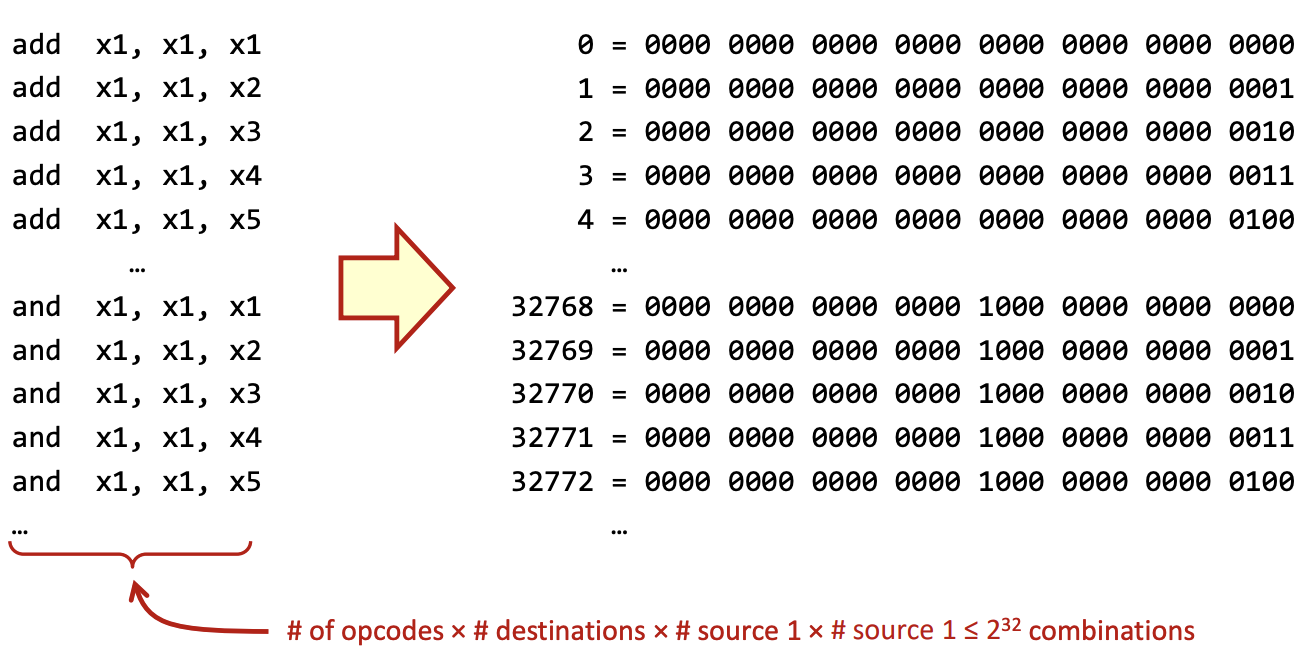
\includegraphics[width=0.65\textwidth]{chapters/chapter1a/images/encoding.png}
\end{center}
\subsubsection*{Fetching}
\begin{center}
    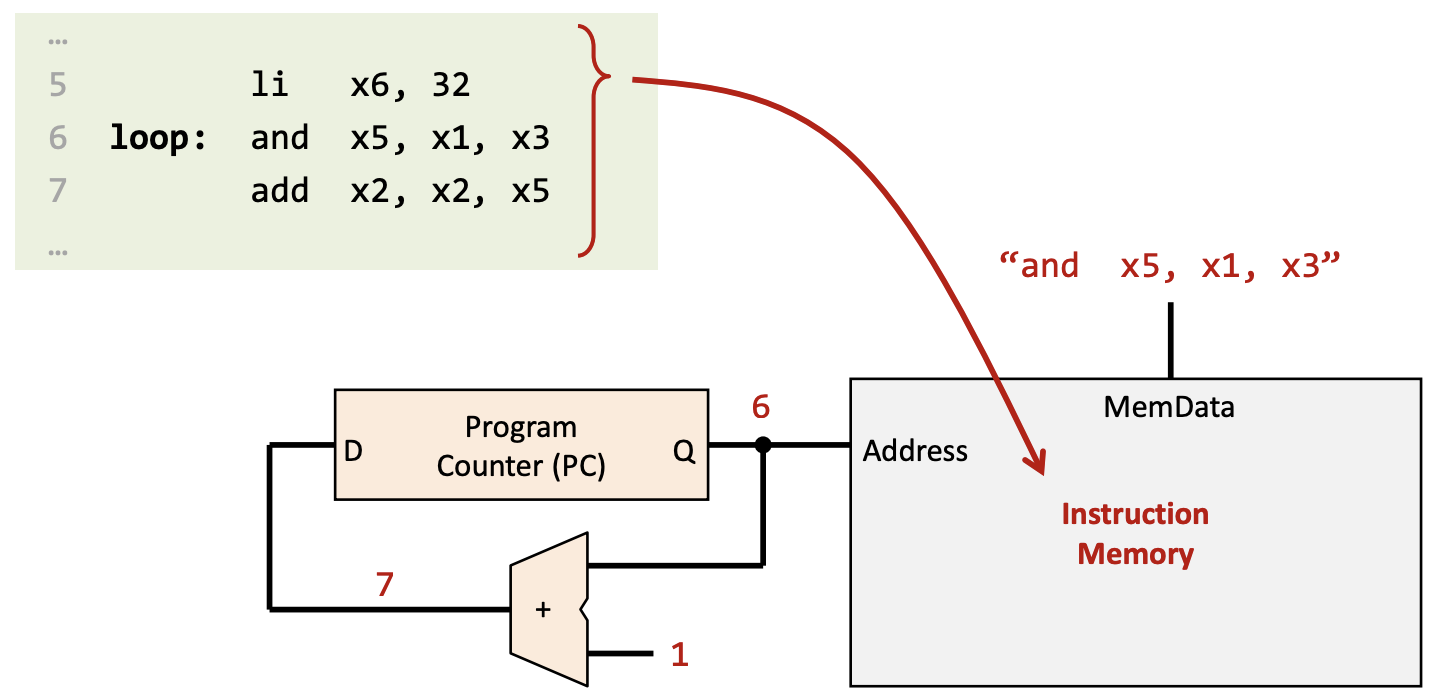
\includegraphics[width=0.65\textwidth]{chapters/chapter1a/images/fetching.png}
\end{center}
\subsubsection*{Executing}
\begin{center}
    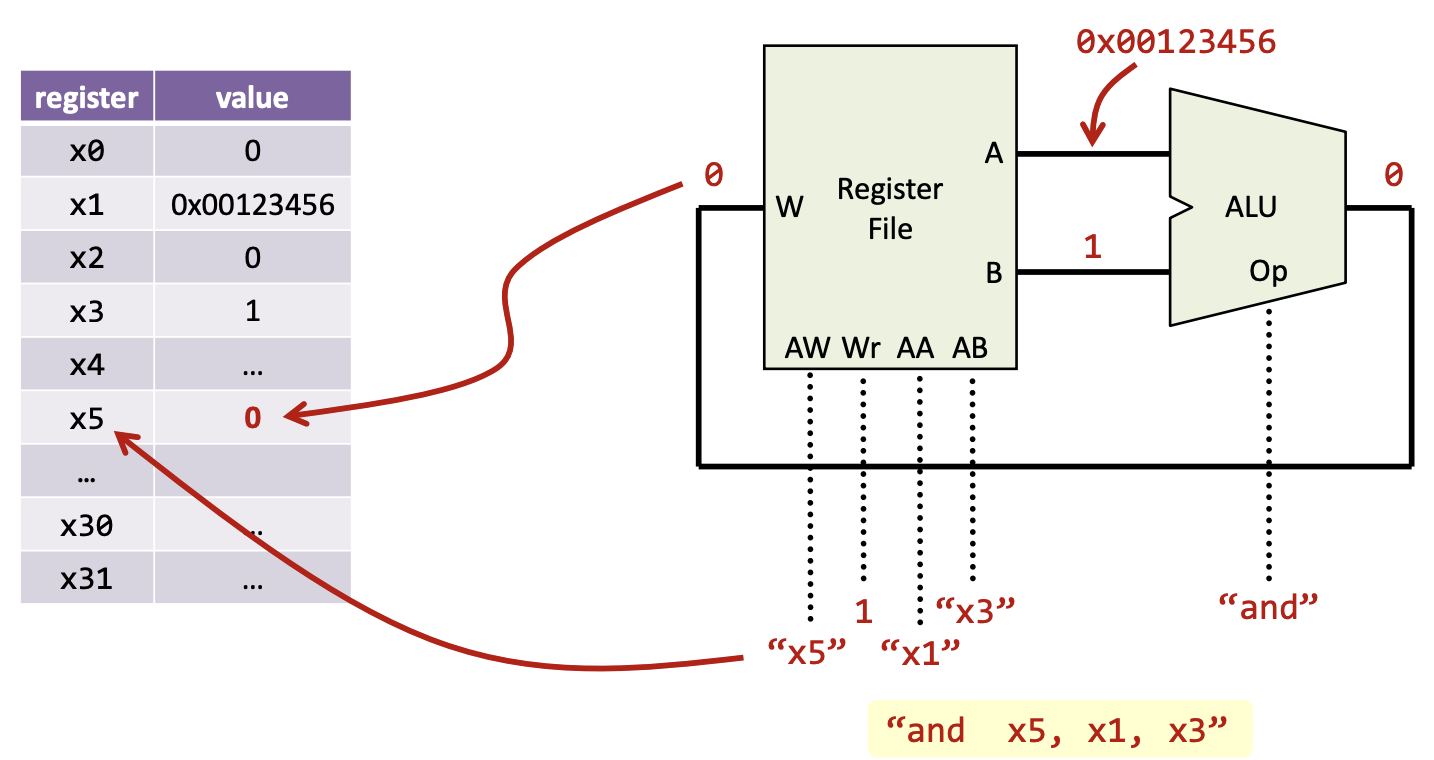
\includegraphics[width=0.65\textwidth]{chapters/chapter1a/images/executing.png}
\end{center}


\section{Joint or Disjoint Program and Data Memories}
\textit{There are two main types of architectures one called the Harvard Architecture (Where the data and the memory are seperate) and pne called Unified Architecture (where data is shared with the program memory)} \newline
\vspace*{10px}
\begin{minipage}[htp]{0.4\textwidth}
    \texttt{Harvard Architecture} \newline
    \vspace*{2px}
    \centering
    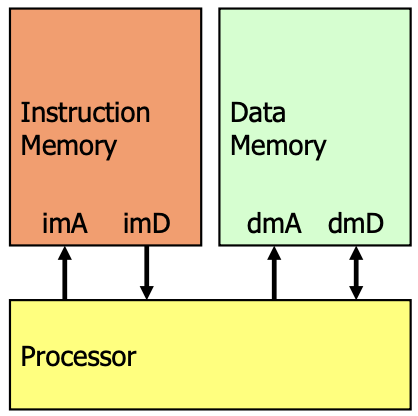
\includegraphics[width=0.6\textwidth]{chapters/chapter1a/images/harvard.png}
\end{minipage}
\hfill
\vline
\hfill
\begin{minipage}[htp]{0.4\textwidth}
    \texttt{Unified Architecture} \newline    
    \vspace*{2px}

    \centering
    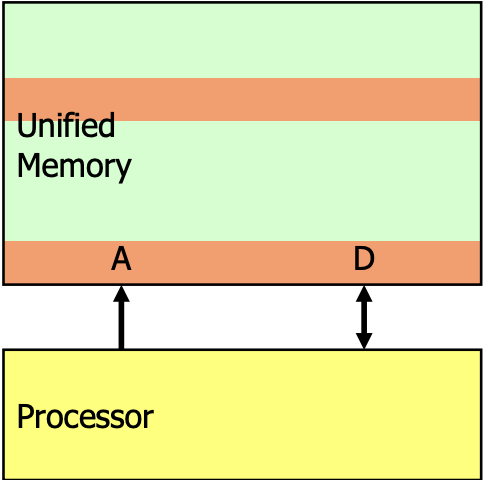
\includegraphics[width=0.6\textwidth]{chapters/chapter1a/images/unified.png}
\end{minipage}
\newpage
\section{The Encoding problem}
\textit{We may ask ourselves how we encode assembly written instructions into actual 0s and 1s.} \newline
\subsection{The Stupid Solution}
\textit{Now, the professor throws out the "stupid idea"(his words) of just counting all possible instructions, assigning a number to each one, and writing the numbers in binary. The problem with such a method is that the number of instructions could grow exponentially, requiring an unmanageable number of bits to represent each one, leading to inefficiency.} \newline 
\begin{center}
    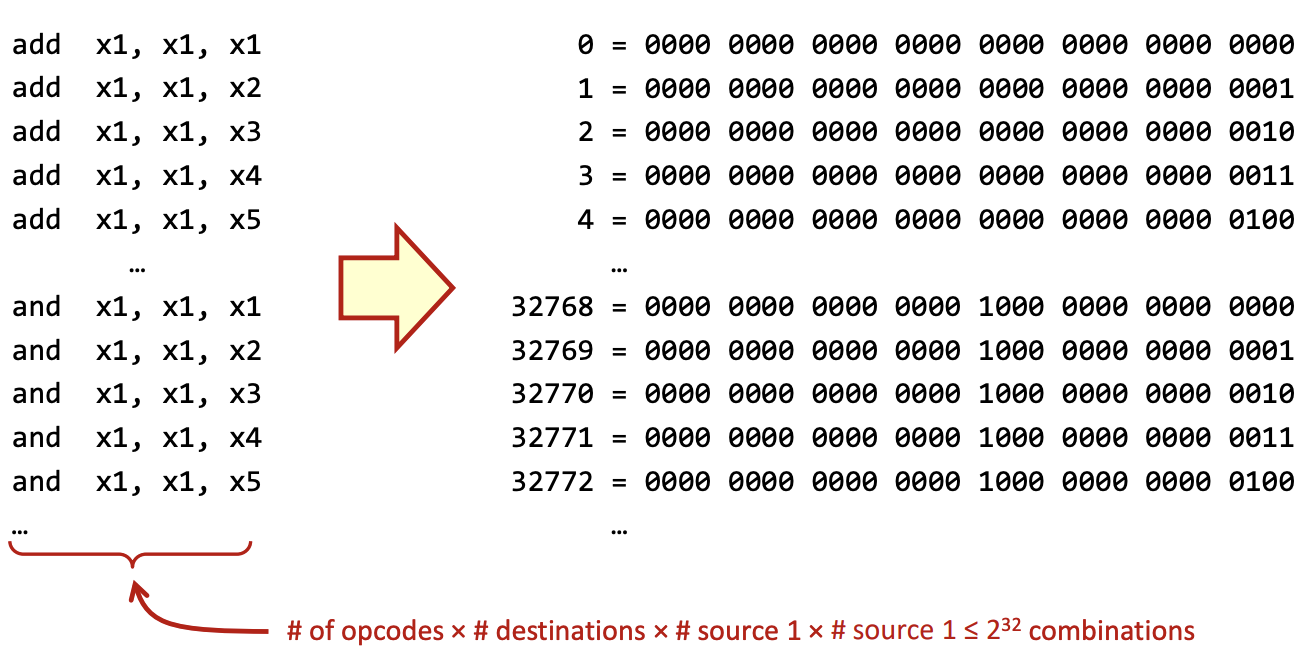
\includegraphics[width=0.7\textwidth]{chapters/chapter1a/images/encoding.png}
    \centering
    \textbf{"stupid solution"}
\end{center}

\subsection{RISC-V Encoding (The Solution)}
\textbf{Instead, the chosen solution is to use an instruction set encoding where instructions are grouped into classes, each with a fixed format optimizing both memory usage and processing speed by limiting the number of bits required to represent instructions.} \newline
\begin{center}
    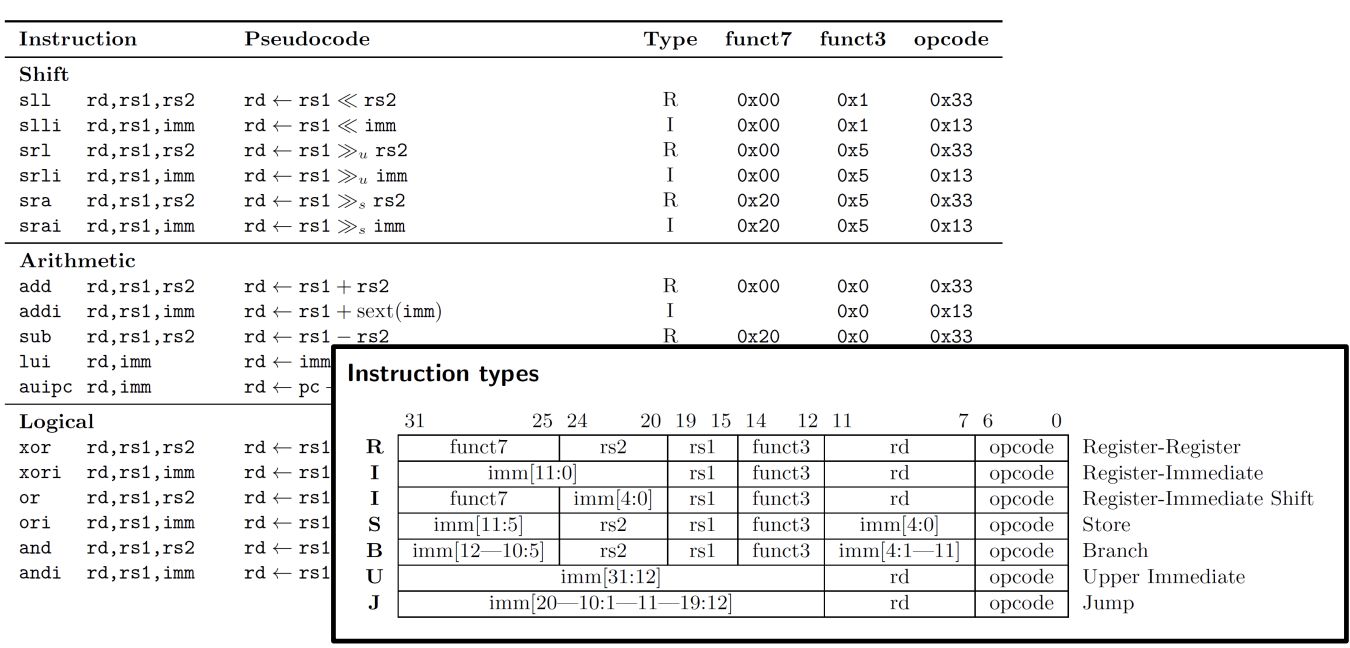
\includegraphics[width=0.7\textwidth]{chapters/chapter1a/images/riscv.png}
    \centering
    \textbf{RISC-V encoding}
\end{center}

\newpage
\subsection{Automating this process}
\textit{Now to automate the processes of decoding assembler code into machine code we use an \textbf{Assembler}, and to automate the process of decoding a higher level language to assembler we use a \textbf{Compiler}}. \newline
\subsubsection{Assembler}
\textit{The program that does this is called an assembler. It takes the assembly code and converts it into machine code.} \newline
\begin{center}
    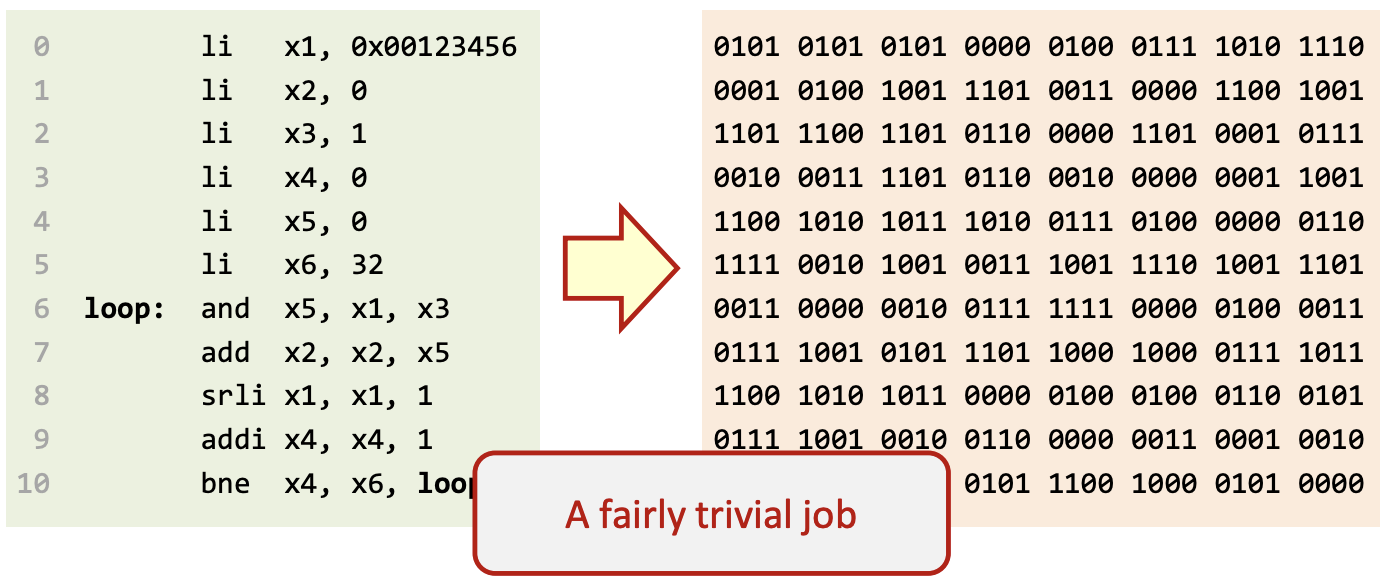
\includegraphics[width=0.7\textwidth]{chapters/chapter1a/images/assembler.png}
    \centering
    \textbf{Assembly}
\end{center}
\subsubsection{Compiler}
A compiler is a program that translates high-level source code written in languages like C or Java into machine code or an intermediate representation. 
\begin{center}
    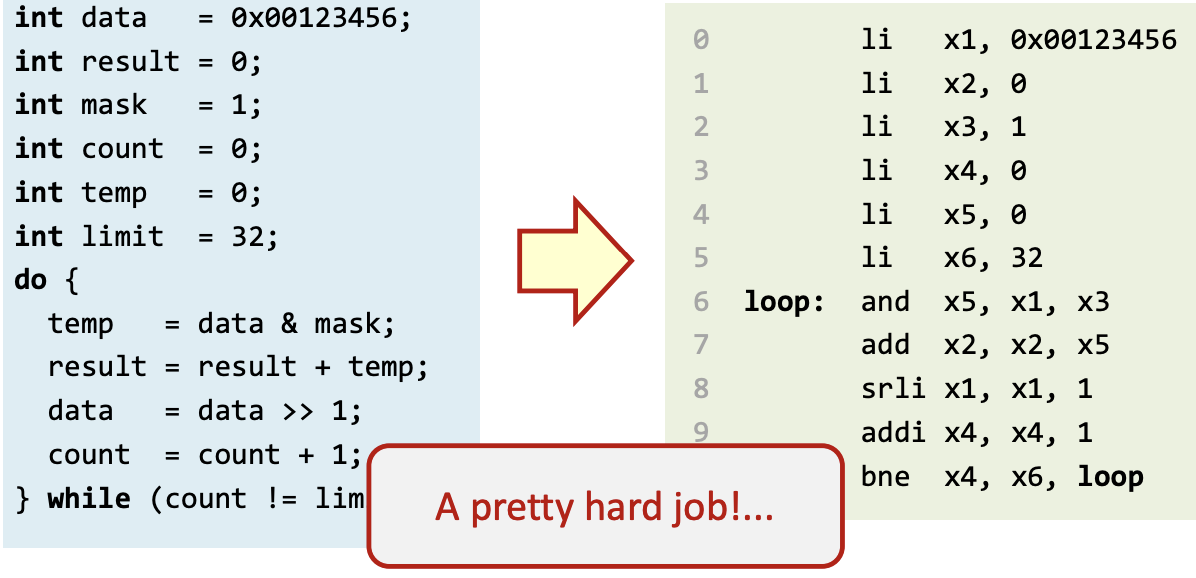
\includegraphics[width=0.7\textwidth]{chapters/chapter1a/images/compiler.png}
    \centering
    \textbf{Compilation}
\end{center}


\section{ISA (Instruction Set Architecture)}
\textit{The ISA is the interface between the hardware and the software. It defines the instructions that a processor can execute, as well as the format of those instructions.} \newline
\begin{center}
    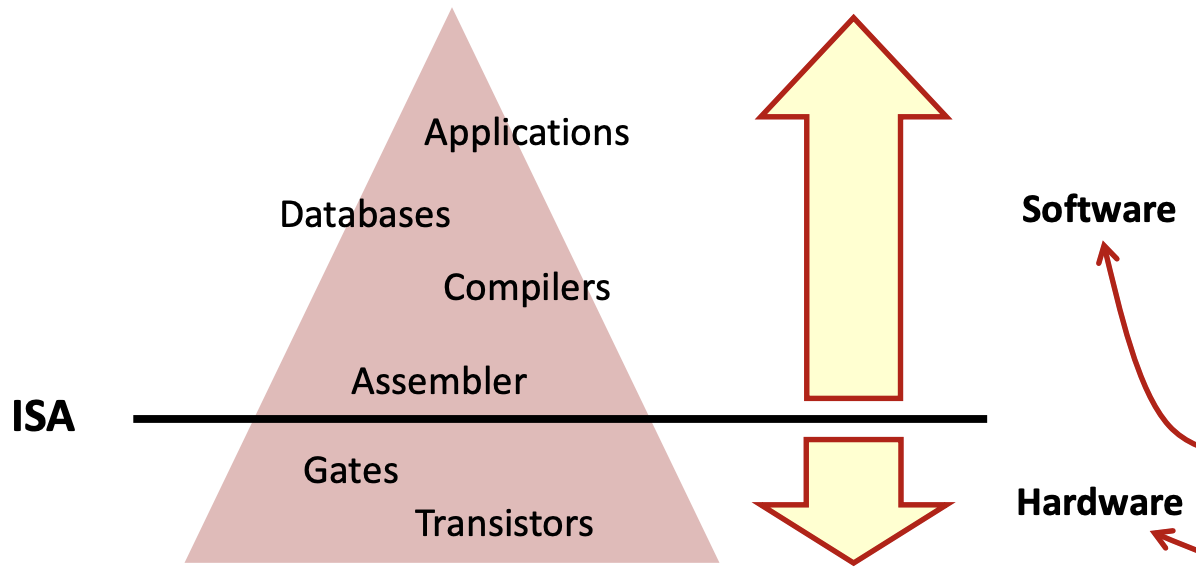
\includegraphics[width=0.65\textwidth]{chapters/chapter1a/images/isa.png}
    \centering
\end{center} % Including chapter0.tex from chapters folder
\chapter{Part I(b) - ISA, Functions, and Stack - W 1.2}
\section{Arithmetic and Logic Instructions in RISCV}
\textit{Bellow some examples of RISCV instructions:} \\
\textbf{Two Operands Instructions} \\
\vspace*{10px}
\begin{minipage}{0.4\textwidth}
\begin{assembly}
sll  x5, x5, x9
add  x6, x5, x7
xor  x6, x6, x8
slt  x8, x6, x7
\end{assembly}
\end{minipage}%
\hfill
\vline
\hfill
\begin{minipage}{0.5\textwidth}
\small
\textit{Shift x5 left by x9 positions $\rightarrow$ x5} \\
\textit{Add x5 and x7 $\rightarrow$ x6} \\
\textit{Logic XOR bitwise x6 and x8 $\rightarrow$ x6} \\
\textit{Set x8 to 1 if x6 is lower than x7, otherwise to 0}
\end{minipage}

\textbf{Arithmetic Instructions} \\
\vspace*{10px}
\begin{minipage}{0.4\textwidth}
\begin{assembly}
slli x5, x5, 3
addi x6, x5, 72
xori x6, x6, -1
slti x8, x6, 321
\end{assembly}
\end{minipage}%
\hfill
\vline
\hfill
\begin{minipage}{0.5\textwidth}
\small
\textit{Shift x5 left of 3 positions $\rightarrow$ x5} \\
\textit{Add 72 to x5 $\rightarrow$ x6} \\
\textit{Logic XOR bitwise x6 and 0xFFFFFFFF $\rightarrow$ x6} \\
\textit{Set x8 to 1 if x6 is lower than 321, to 0 otherwise} \\
\end{minipage} \\
\textbf{Here, you may ask yourself, why are all immediates (constants) writtent on a maximum of 12bits?} \\
\subsection{Constants must be encoded on 12 bits}
\textit{As you may see here, all instructions encode immediates on 12 bits.}
\begin{center}
    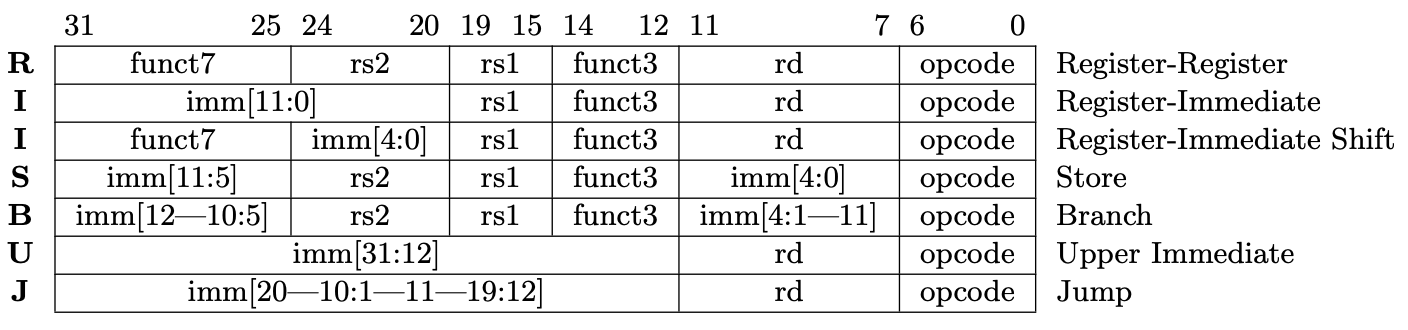
\includegraphics[width=0.8\textwidth]{chapters/chapter1b/images/riscv.png}
\end{center}

\subsection{Assembler Directives} \textit{Assembler directives help write cleaner and more readable code. The code snippets on the left and right below are equivalent.}

\begin{center} 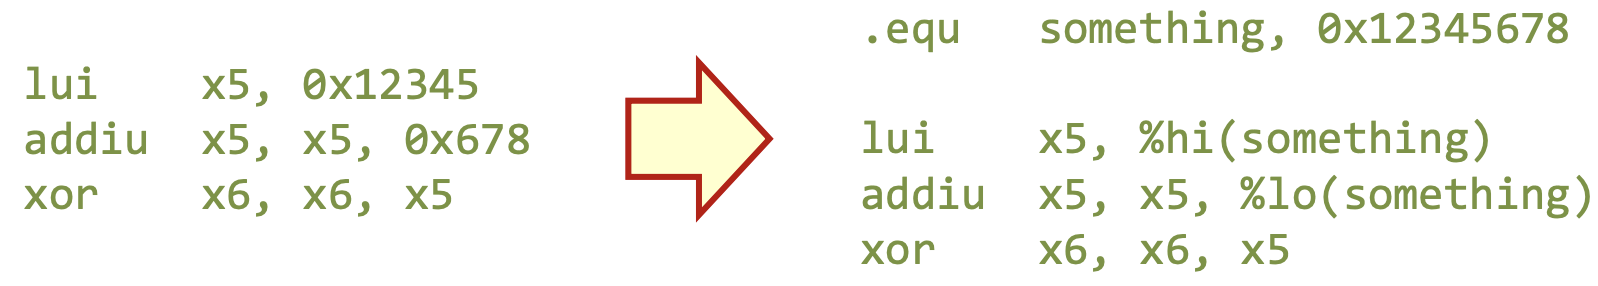
\includegraphics[width=0.65\textwidth]{chapters/chapter1b/images/directives.png} \end{center}

The left-hand side code snippet shows an assembly sequence where a 32-bit constant value (\texttt{0x12345678}) is loaded into a register (\texttt{x5}). Since immediate values are 16-bit limited, this requires splitting the 32-bit value into two instructions: 

\begin{itemize}
    \item[-] The first instruction, \texttt{lui}, loads the upper 16 bits (\texttt{0x12345}) into the register \texttt{x5}.
    \item[-] The second instruction, \texttt{addiu}, adds the lower 16 bits (\texttt{0x678}) to \texttt{x5}, completing the full 32-bit value in the register.
\end{itemize}

\textit{This approach, while functional, can become cumbersome when dealing with multiple constants, making the code less readable and harder to maintain. \\
} 
\vspace*{5px}
The right-hand side shows the same functionality but makes use of assembler directives, specifically the \texttt{.equ} directive to define a label (\texttt{something}) for the constant \texttt{0x12345678}. Using the \texttt{\%hi()} and \texttt{\%lo()} pseudo-instructions, the assembler automatically splits the constant into its upper and lower parts:

\begin{itemize}
    \item[-] The \texttt{\%hi(something)} loads the upper 16 bits into \texttt{x5}.
    \item[-] The \texttt{\%lo(something)} adds the lower 16 bits to \texttt{x5}.
\end{itemize}

This method enhances code clarity and maintainability, especially when working with multiple constants, by using human-readable labels instead of raw numeric values. The assembler handles the details of splitting the 32-bit constant into its upper and lower parts.
\begin{center} 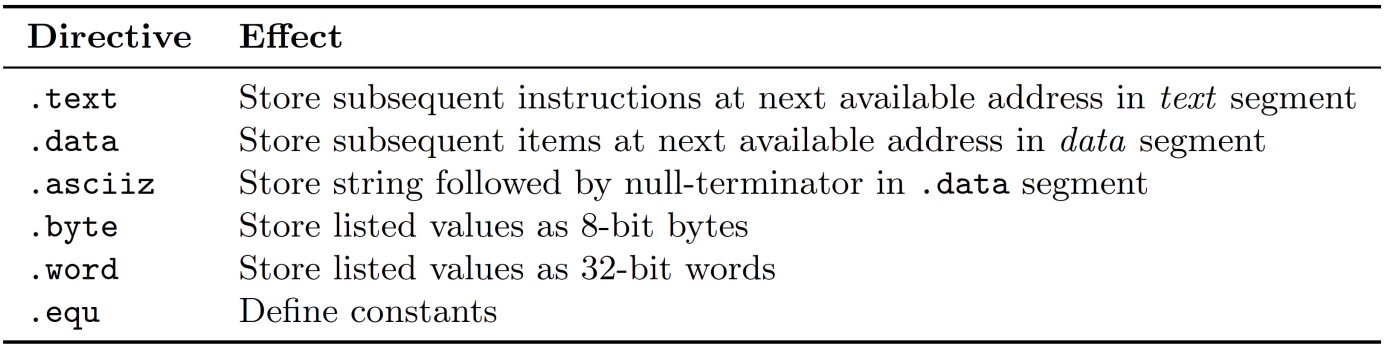
\includegraphics[width=0.65\textwidth]{chapters/chapter1b/images/directives2.png} \end{center}

\subsection{The \texttt{x0} Register} 
\textit{The \texttt{x0} register is hardwired to 0 and cannot be changed.} \ \textit{Any attempt to write into \texttt{x0} will have no effect.}

\texttt{Why is this useful?} \\
One common application is in introducing wait delays during program execution. By leveraging the fixed nature of \texttt{x0}, it simplifies certain instructions that require an immediate zero value.

\section{PseudoInstructions}
\textit{PseudoInstructions simplify commands involving the \texttt{x0} register by creating easier-to-use alternatives.} \newline
\begin{center}
        \begin{tabular}{|c|c|c|}
        \hline
        \textbf{Pseudoinstruction} & \textbf{Base Instruction(s)} & \textbf{Meaning} \\ \hline
        \texttt{nop}               & \texttt{addi x0, x0, 0}      & No operation     \\ \hline
        \texttt{li rd, immediate}  & Myriad sequences             & Load immediate   \\ \hline
        \texttt{mv rd, rs}         & Myriad sequences             & Copy register    \\ \hline
        \texttt{not rd, rs}        & \texttt{xori rd, rs, -1}     & One's complement \\ \hline
        \texttt{neg rd, rs}        & \texttt{sub rd, x0, rs}      & Two's complement \\ \hline
        \texttt{seqz rd, rs}       & \texttt{sltiu rd, rs, 1}     & Set if = zero    \\ \hline
        \texttt{snez rd, rs}       & \texttt{sltu rd, x0, rs}     & Set if $\neq$ zero    \\ \hline
        \texttt{sltz rd, rs}       & \texttt{slt rd, rs, x0}      & Set if < zero    \\ \hline
        \texttt{sgtz rd, rs}       & \texttt{slt rd, x0, rs}      & Set if > zero    \\ \hline
        \end{tabular}
\end{center} 
The term \textit{myriad sequences} refers to a series of instructions that together achieve the functionality of a single pseudoinstruction, such as using \texttt{lui} and \texttt{addi} to implement \texttt{li rd, immediate}.

\textbf{According to the professor li should be called \texttt{mvi} (as move immediate).}

\subsection{Control flow instructions}
\textit{Control flow instructions are used to change the order of execution of instructions are a kind of pseudo-instructions.}
\begin{assembly}
    li x1, 0x00123456
    li x2, 0
    li x3, 1
    li x4, 0
    li x5, 0
    li x6, 32
loop: and x5, x1, x3
    add x2, x2, x5
    srli x1, x1, 1
    addi x4, x4, 1
    bne x4, x6, loop
\end{assembly}

\subsection{If-Then-Else}
\begin{minipage}[htp]{0.4\textwidth}
\begin{cc}
if (x5 == 72) {
    x6 = x6 + 1;
    } else {
    x6 = x6 - 1;
}
\end{cc}    
\end{minipage}
\hfill
\vline
\hfill
\begin{minipage}[htp]{0.4\textwidth}
\begin{assembly}
.text
    li x7, 72
    beq x5, x7, then_clause
else_clause:
    addi x6, x6, -1
    j end_if
then_clause:
    addi x6, x6, 1
end_if:
\end{assembly}
\end{minipage} \\
\vspace*{5px}
\textit{As seen here, beqi does not exist in RISCV, instead we use \texttt{beq} and \texttt{li} to achieve the same result.}
\subsection{Jumps and Branches}
A common but not universal distinction exists between \emph{jumps} and \emph{branches}. In RISC-V (inherited from MIPS and used by SPARC, Alpha, etc.), jumps refer to unconditional control transfer instructions, while branches refer to conditional control transfer instructions. However, not all architectures follow this convention. For instance, in x86, all control transfer instructions are considered jumps, such as \texttt{JMP}, \texttt{JZ}, \texttt{JC}, and \texttt{JNO}.

\subsection{Comparaisions}
\textit{The processor implements only $<$ and $>$, and the assembler “creates” $\leq$ and $\geq$.}

\begin{center}
    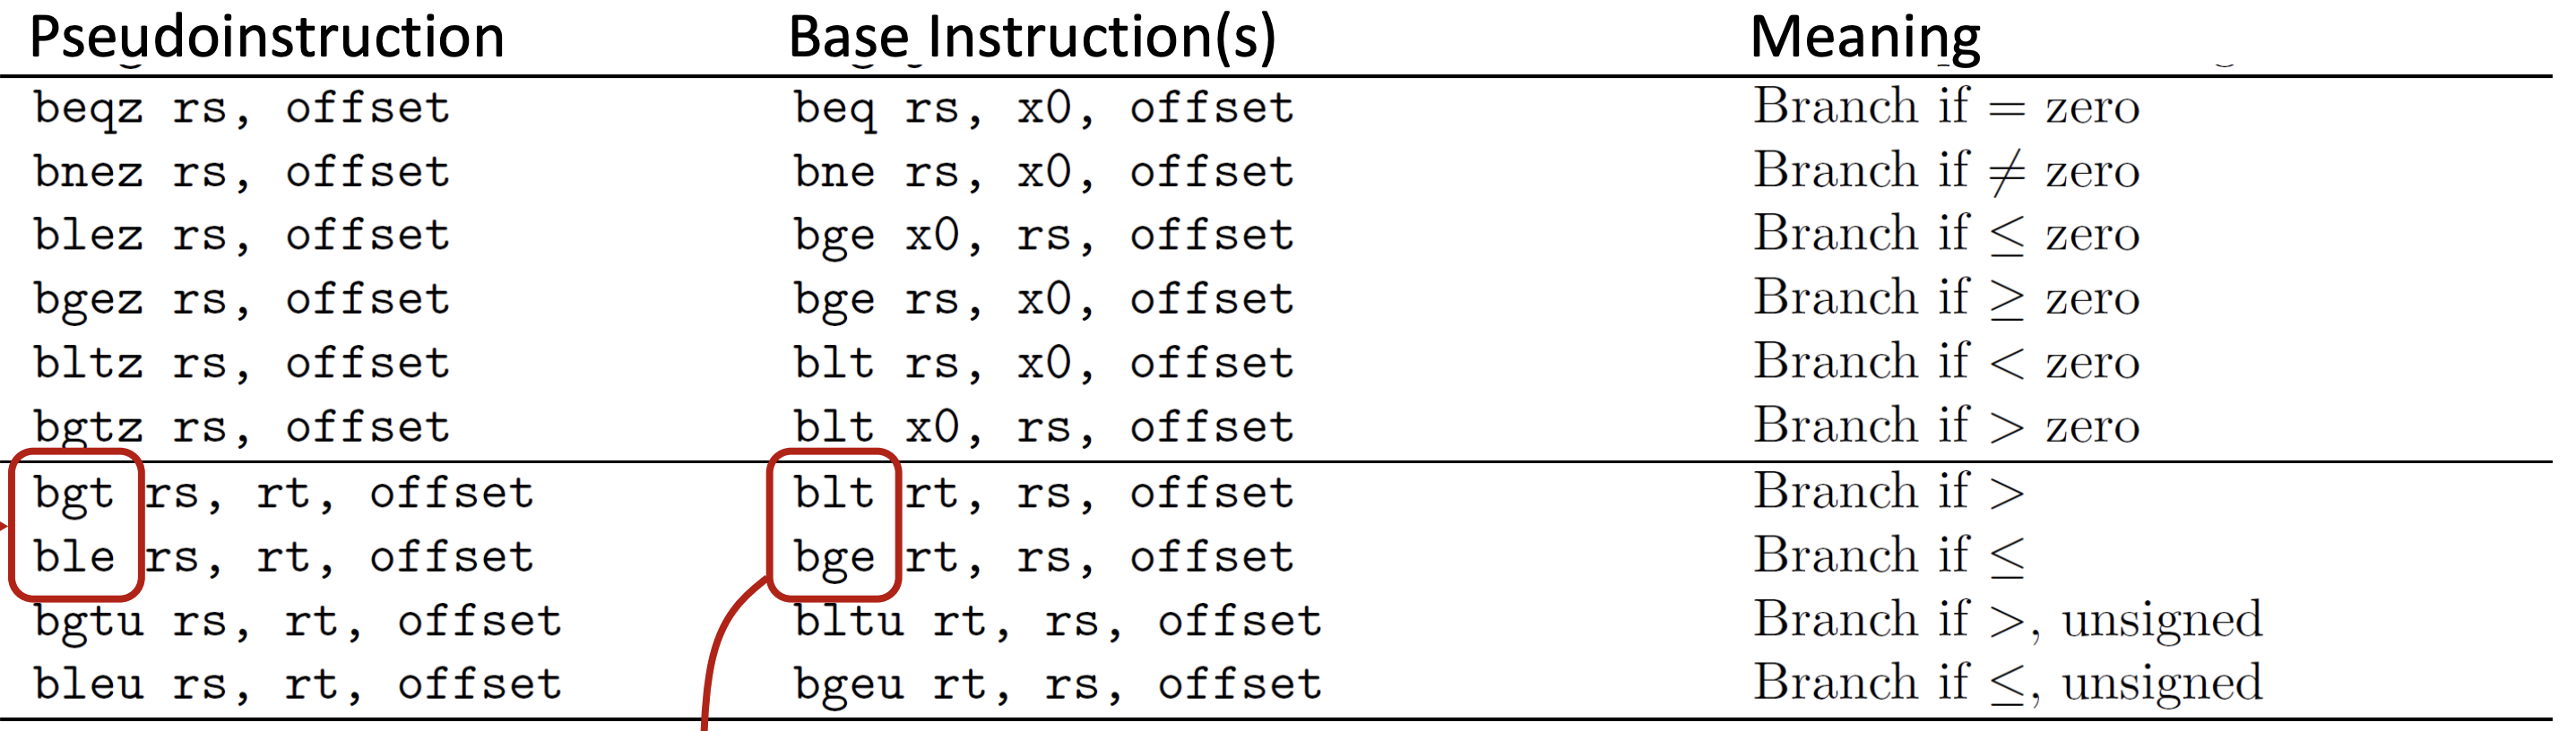
\includegraphics[width=0.75\textwidth]{chapters/chapter1b/images/comp.png}
\end{center}
\subsection{Do-While}
\textit{Do-while loops look like this (we obviously use control flow instructions here).} \\
\begin{minipage}[htp]{0.4\textwidth}
\begin{cc}
do {
    x5 = x5 >> 1;
    x6 = x6 + 1;
} while (x5 != 0);
\end{cc}    
\end{minipage}
\hfill
\vline
\hfill
\begin{minipage}[htp]{0.4\textwidth}
\begin{assembly}
.text
loop:
    srli x5, x5, 1
    addi x6, x6, 1
    bnez x5, loop
\end{assembly}
\end{minipage}

\section{Functions}
\textit{In higher-level programming languages, functions (routines, subroutines, procedures, methods, etc.) are used to encapsulate code and make it reusable. } \\
\textbf{Calling a function involves these steps:}
\begin{enumerate}
    \item Place arguments where the called function can access them.
    \item Jump to the function.
    \item Acquire storage resources the function needs.
    \item Perform the desired task of the function.
    \item Communicate the result value back to the calling program.
    \item Release any local storage resources.
    \item Return control to the calling program.
\end{enumerate}
\subsection{Jump to the Function/Retun control to the calling program}
\subsubsection{The too simple not working approach}
A simple (not working) approach for creating functions would be to do this: 
\begin{center}
    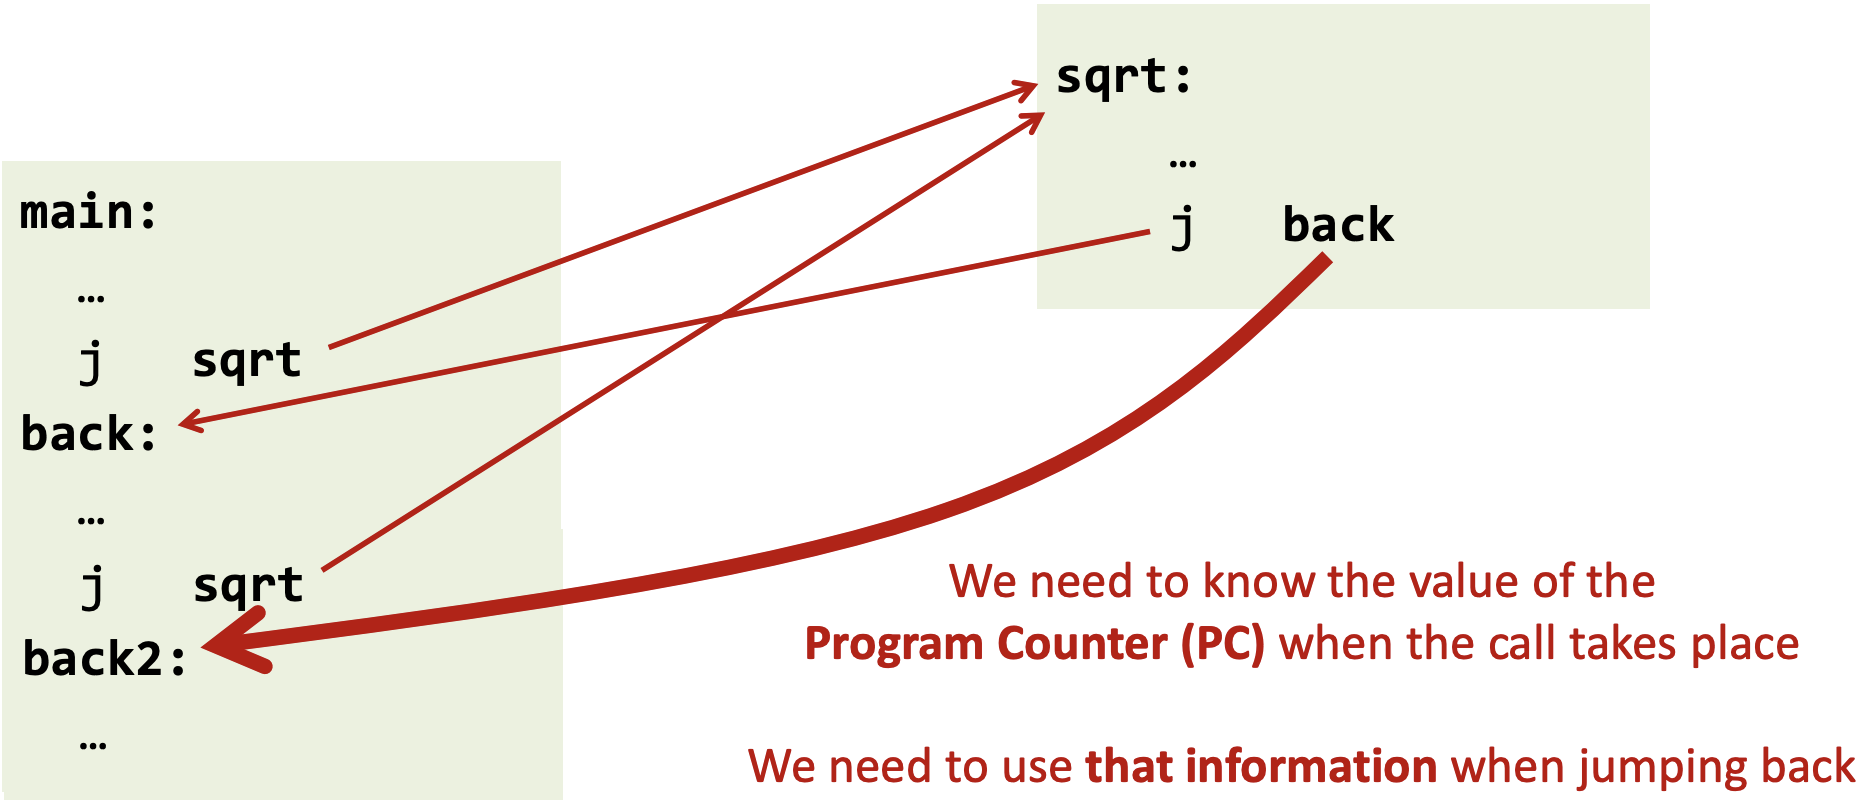
\includegraphics[width=0.75\textwidth]{chapters/chapter1b/images/function.png}
\end{center}
\textit{With this approach the function doesn't know where to return to after being called (back2 or back)}
\textbf{For the next part, remember, the Program Counter is distinct from general-purpose registers. It is dedicated to managing the flow of instruction execution, while general registers are used for data manipulation. }
\subsubsection{The Good Approach}
\textit{The right approach involves using the Jump and Link instruction \texttt{jal}, here loading PC + 4 (remember 4 bytes per Instruction) into x1 as a way to come back from the function.} \\
\begin{minipage}[htp]{0.4\textwidth}
\begin{assembly}
main:
    ...
    jal x1, sqrt
    ...
    ...
    jal x1, sqrt
\end{assembly}    
\end{minipage}
\hfill
\vline
\hfill
\begin{minipage}[htp]{0.4\textwidth}
\begin{assembly}
sqrt:
    ...
    ...
    jr x1
\end{assembly}
\end{minipage} \\
\textit{Both times x1 was used to store the return adress, and there is a reason for that (Register Conventions Sections).}

\subsection{Jump Instructions}
\textit{There are only two core real jump instructions in RISCV, \texttt{jal} (jump and link) and \texttt{jalr} (jump and link register), the rest are pseudo instructions using them.} \\

\begin{center}
    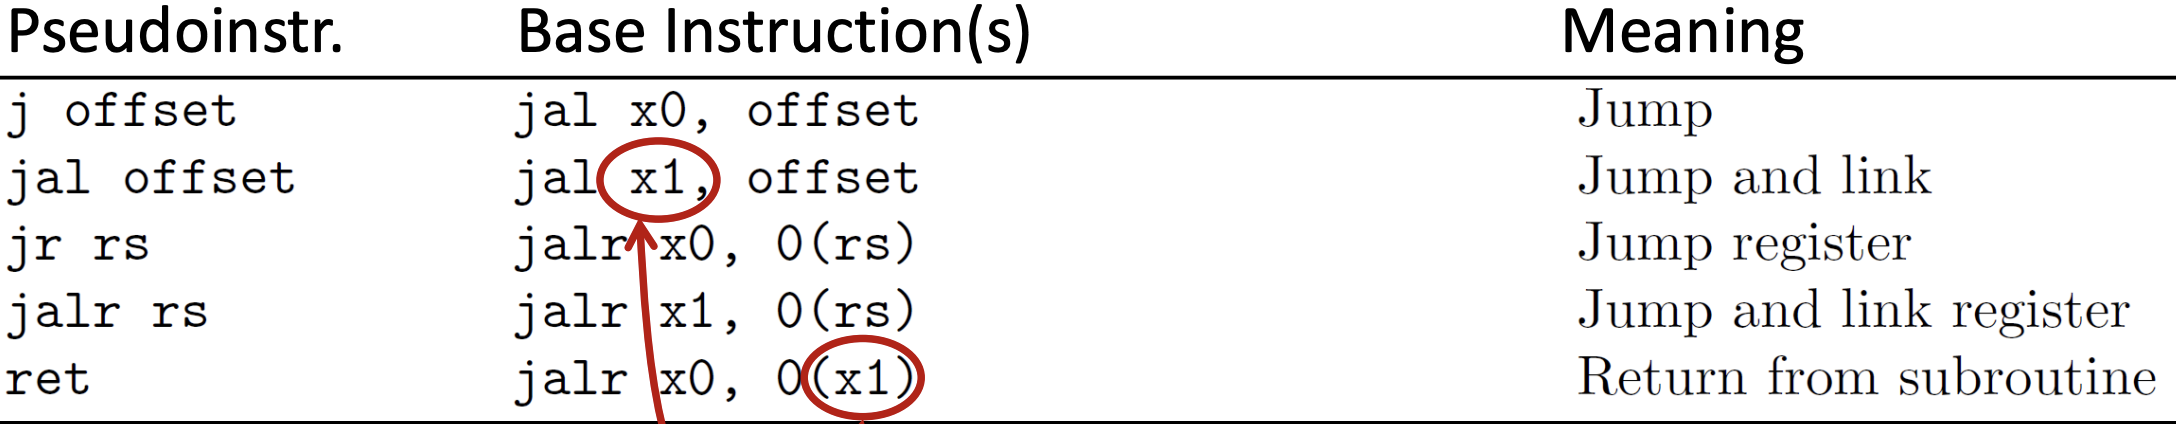
\includegraphics[width=0.75\textwidth]{chapters/chapter1b/images/jump.png}
\end{center}
\newpage
\subsection{Register Conventions}
\textit{Register conventions are rules that dictate how registers are used in a program, here are the ones we've seen for now} \\
\begin{center}
    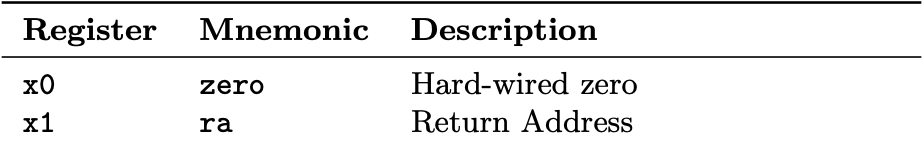
\includegraphics[width=0.75\textwidth]{chapters/chapter1b/images/conventions.png}
\end{center}

\subsection{Back to the good (not so good) approach}
\textit{There's still a problem with the previous approach, say for example you want to call a function from another function.}
\begin{center}
    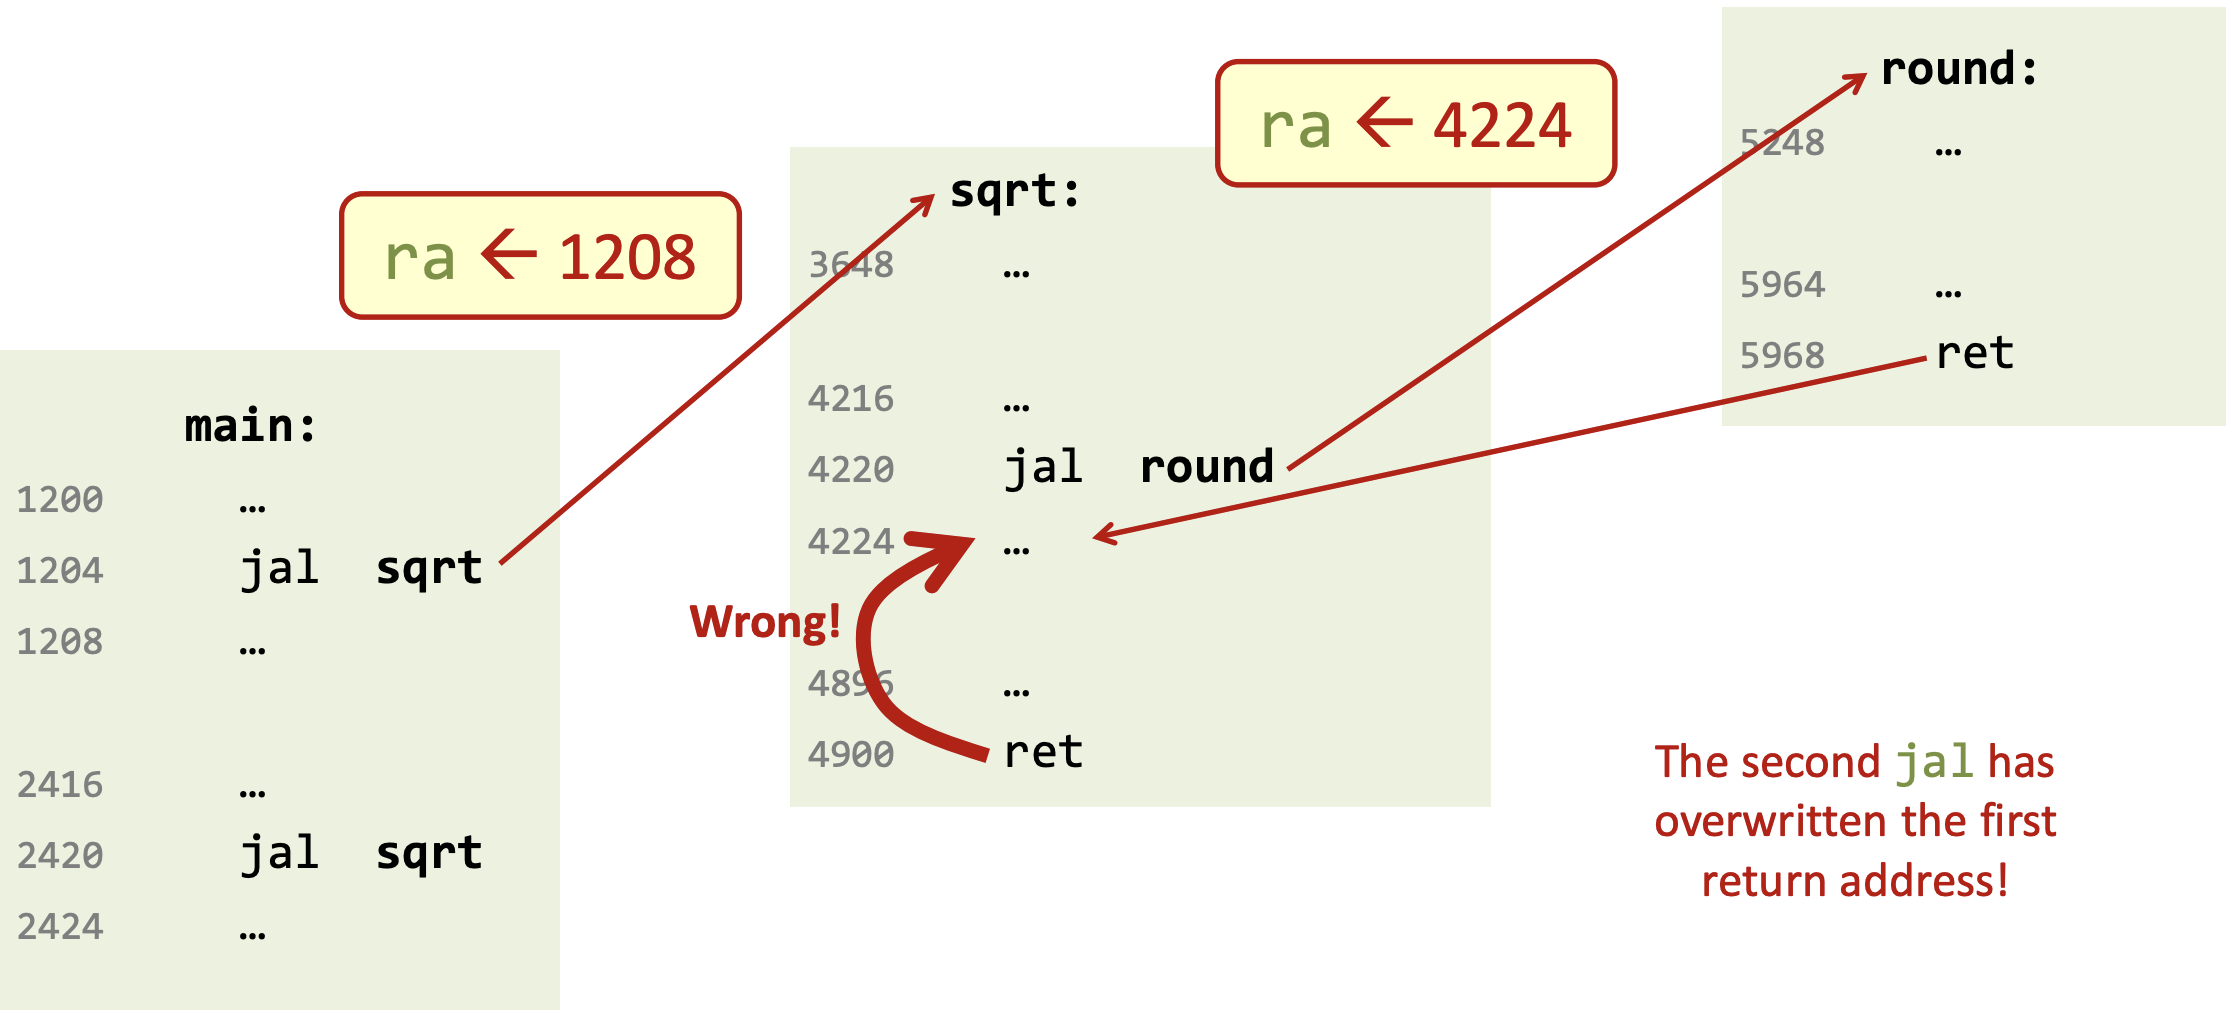
\includegraphics[width=0.75\textwidth]{chapters/chapter1b/images/function2.png}
\end{center}
\textbf{Here the allocated space for the return address is overwritten by the second function call, and the first function can't return to the right place.}
\subsection{One simple solution (still not good)}
\textit{One solution would be to say that a range of registers are used for certain functions and that they can't be used by other functions.}
\begin{center}
    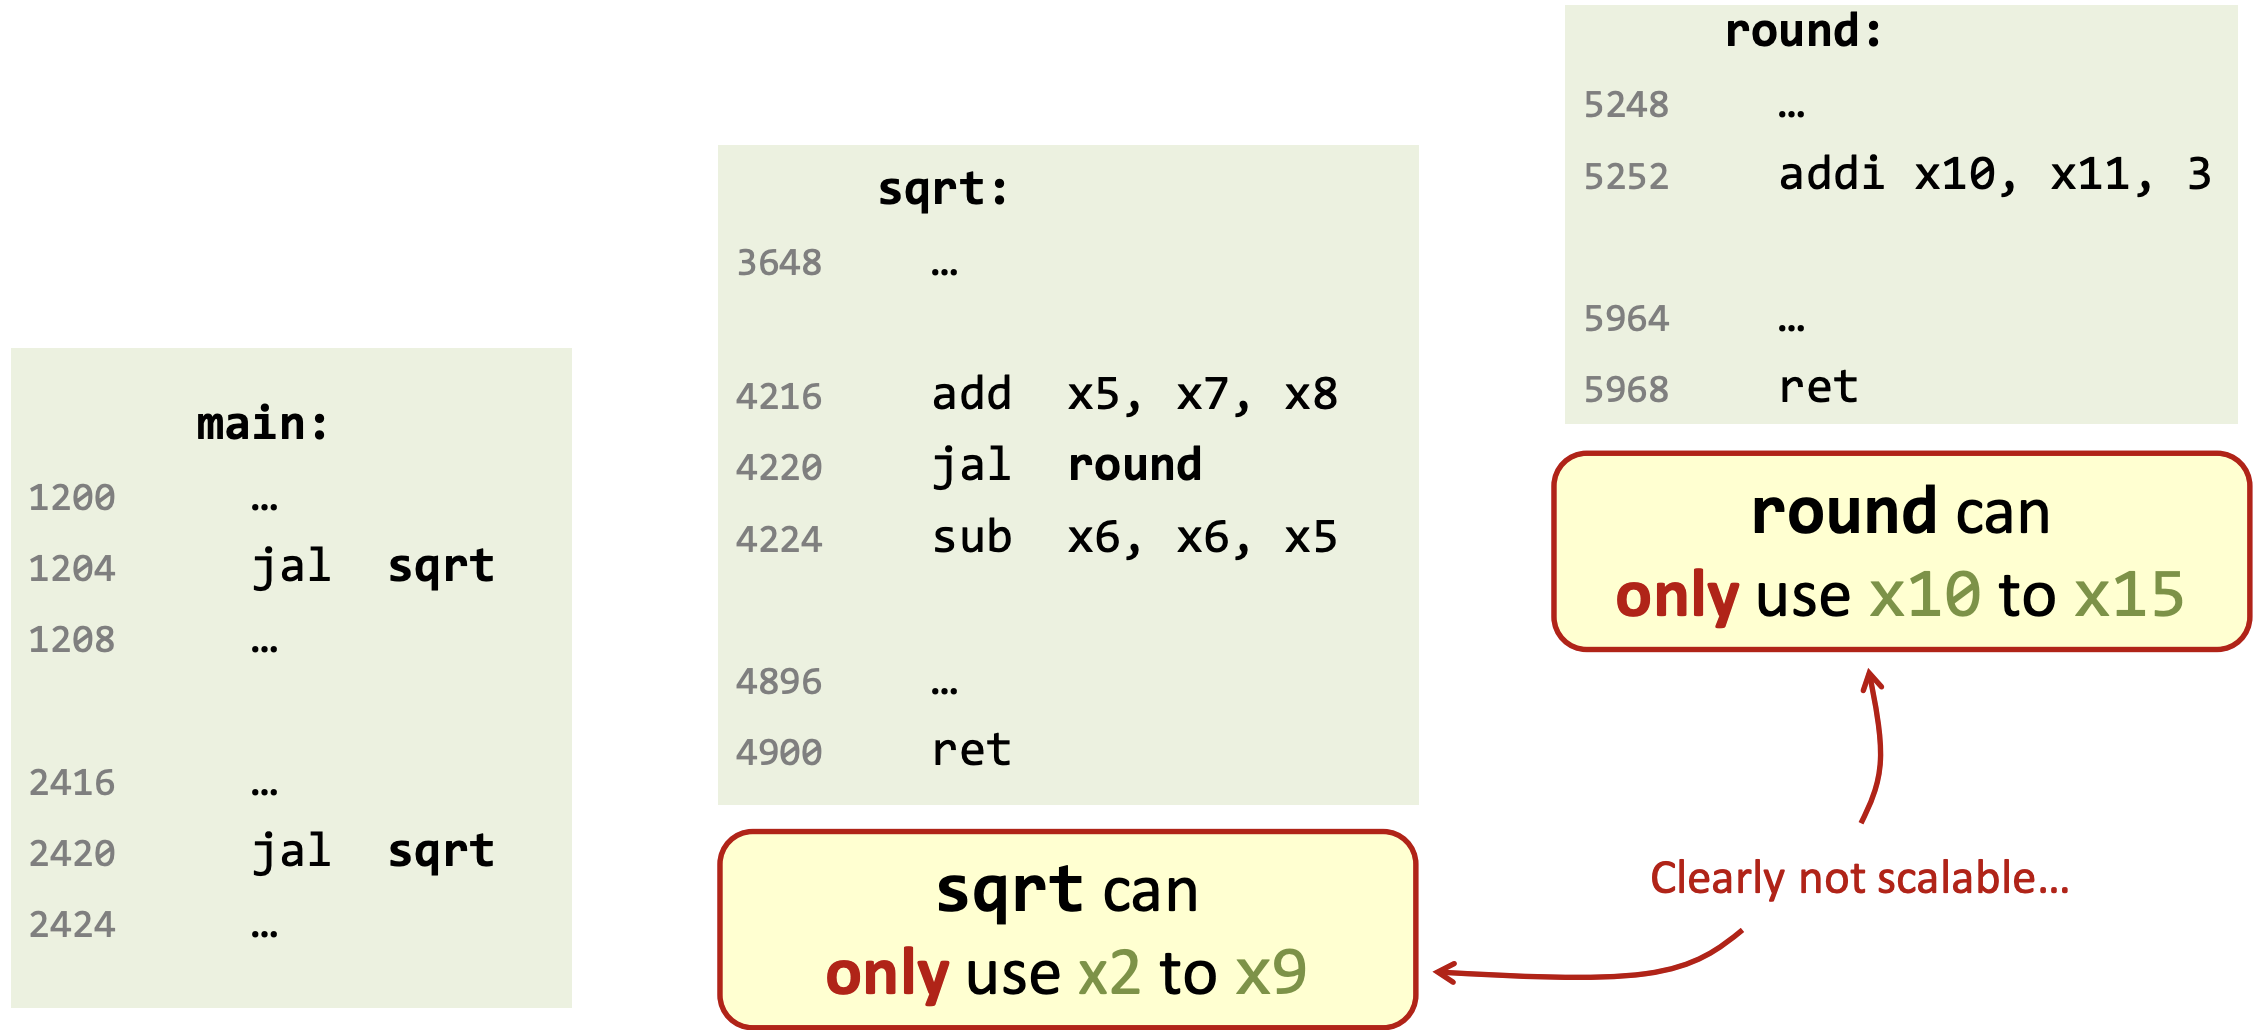
\includegraphics[width=0.75\textwidth]{chapters/chapter1b/images/function3.png}
\end{center}
\textbf{The problem here is that it's still not very scalable.}
\subsection{Acquire storage resources the function needs (still not it)}
One simple solution to our problem would be to allocate memory for the function at in the data section of the program. \\
\begin{minipage}[htp]{0.4\textwidth}
\begin{assembly}
.data
sqrt_save_ra: .word 0
sqrt_save_x5: .word 0 
\end{assembly}
\end{minipage}
\hfill
\vline
\hfill
\begin{minipage}[htp]{0.4\textwidth}
\begin{assembly}
.text
sqrt:
...
add x5, x7, x8
sw ra, sqrt_save_ra
sw x5, sqrt_save_x5
jal round
lw ra, sqrt_save_ra
lw x5, sqrt_save_x5
sub x6, x6, x5
...
ret
\end{assembly}
\end{minipage}
\subsubsection{Problem: Recursive Functions}
\textit{The problem here is that the return address is overwritten by the recursive call.}
\begin{center}
\begin{assembly}
.data
    find_child_save_ra: .word 0
.text
    find_child:
    ...
    sw ra, find_child_save_ra
    jal find_child
    lw ra, find_child_save_ra
    ...
    ret
\end{assembly}
\end{center}
\subsection{The Stack}
\textit{The Solution to our Problem is this, the Stack.} \\
\textbf{The Stack is a region of memory that grows and shrinks as needed.} \\
We may use a register (e.g \texttt{x2}) to point to the first used word after the end of the used region.
\begin{center}
    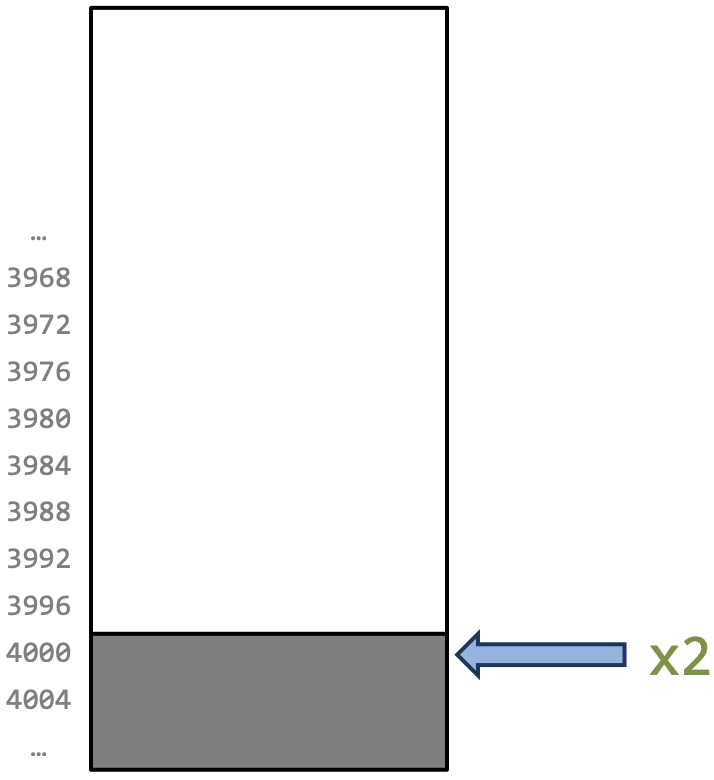
\includegraphics[width=0.4\textwidth]{chapters/chapter1b/images/stack.png}
\end{center}

\subsubsection{Dynamic Memory Allocation}
The Stack, contrary to the Data Section, is dynamic and can be used to allocate memory when needed. This means that during program execution, variables or temporary data can be stored in the stack, which grows or shrinks depending on the operations performed. \\
 The \texttt{stack pointer}, typically register x2, is used to manage the allocation and deallocation of memory.

\begin{minipage}[htp]{0.4\textwidth}
\textit{In this instruction, for example, we allocate 12 bytes in the stack. We achieve this by decrementing the stack pointer (x2) by 12. This ensures that the new memory space is available for temporary storage.}
\begin{assembly}
addi x2, x2, -12
\end{assembly}
\end{minipage}
\hfill
\vline
\hfill
\begin{minipage}[htp]{0.4\textwidth}
\begin{center}
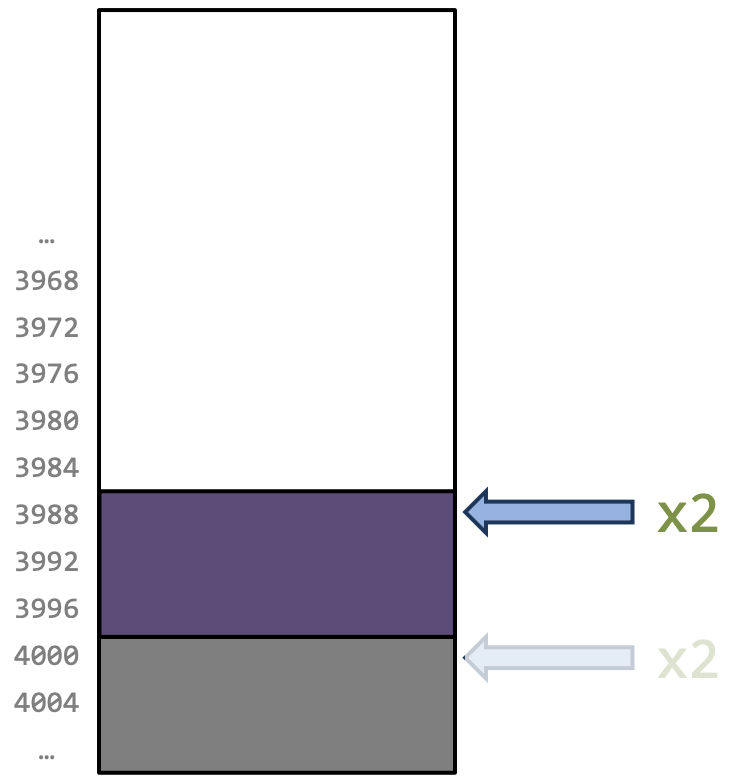
\includegraphics[width=0.75\textwidth]{chapters/chapter1b/images/stack2.png}
\end{center}
\end{minipage}

\subsubsection{Retrieving Data from the Stack}
Once memory has been allocated on the stack, we can store or retrieve data from it. In this case, we are retrieving data that was previously saved in the stack. The lw (load word) instruction is used to load the values stored at different offsets in the stack.

\begin{minipage}[htp]{0.4\textwidth}
\textit{In this case, we retrieve three different values from the stack using the lw instruction, which loads a 4-byte value into the specified registers (ra, x5, and x6). The offsets (0, 4, and 8) refer to different positions in the 12 bytes we allocated earlier.}
\begin{assembly}
lw ra, 0(x2)
lw x5, 4(x2)
lw x6, 8(x2)
\end{assembly}
\end{minipage}
\hfill
\vline
\hfill
\begin{minipage}[htp]{0.4\textwidth}
\begin{center}
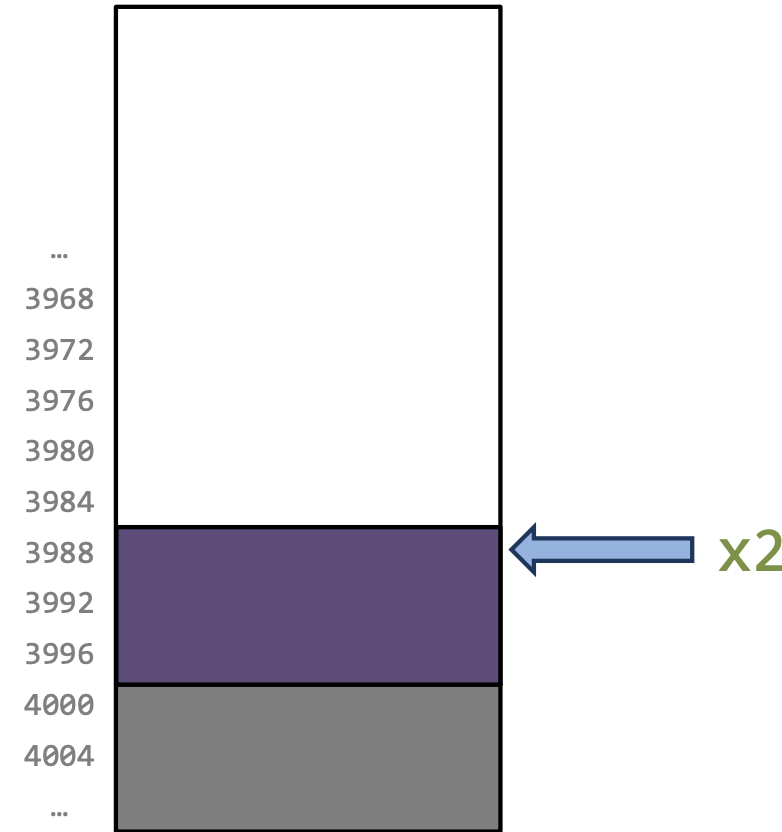
\includegraphics[width=0.75\textwidth]{chapters/chapter1b/images/stack3.png}
\end{center}
\end{minipage}
\newpage

\subsubsection{Memory Deallocation}
After the data has been used or is no longer needed, it is good practice to deallocate the memory to ensure proper management of the stack. We deallocate memory by adjusting the stack pointer (x2) back to its original position.

\begin{minipage}[htp]{0.4\textwidth}
\textit{In this instruction, we restore the stack to its previous state by adding 12 back to the stack pointer (x2).} \\ \textit{This effectively "frees" the 12 bytes of memory we had allocated earlier.}
\begin{assembly}
addi x2, x2, 12
\end{assembly}
\end{minipage}
\hfill
\vline
\hfill
\begin{minipage}[htp]{0.4\textwidth}
\begin{center}
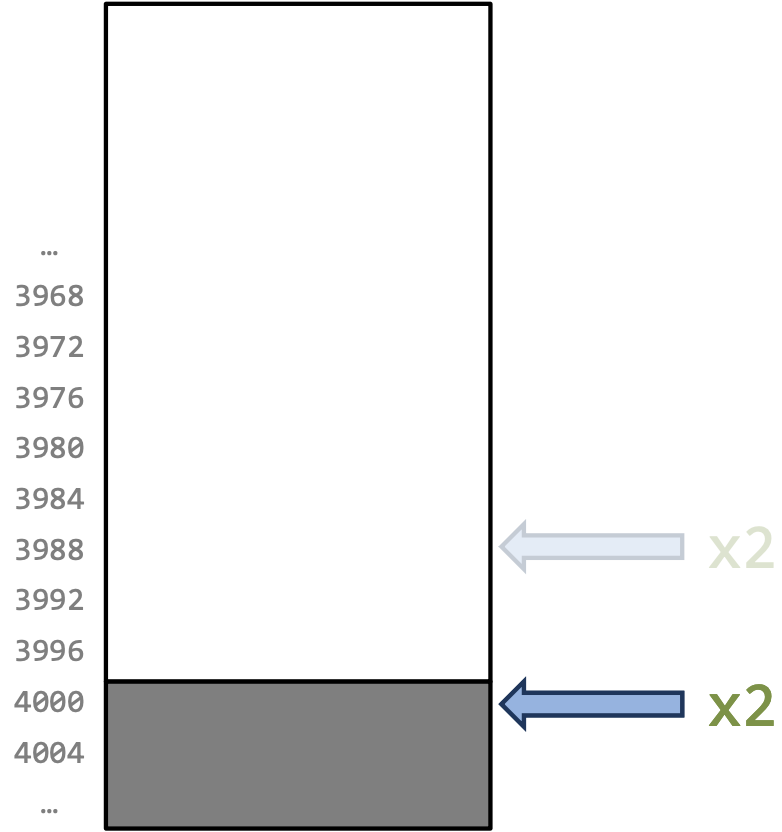
\includegraphics[width=0.75\textwidth]{chapters/chapter1b/images/stack4.png}
\end{center}
\end{minipage}

\subsubsection{The Stack Pointer}
\textit{The Stack Pointer is a register that points to the top of the stack, by convention it corresponds to the x2 register} \\
\begin{center}
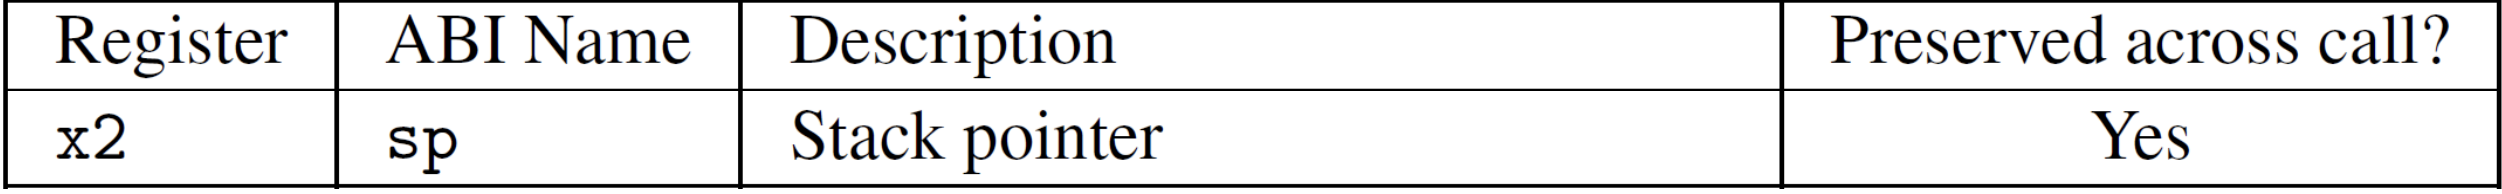
\includegraphics[width=0.75\textwidth]{chapters/chapter1b/images/conventions2.png}
\end{center}
\small
\textit{Other architectures have special instructions to place stuff on
the stack (push) and to retrieve it (pop)} \\
\vspace*{10px}
\begin{minipage}[htp]{0.4\textwidth}
\begin{lstlisting}
PUSH AX
\end{lstlisting}
\end{minipage}
\hfill
\vline
\hfill
\begin{minipage}[htp]{0.4\textwidth}
\begin{assembly}
add sp, sp, -4
sw x5, 0(sp)
\end{assembly}
\end{minipage}

\subsection{Spilling Registers to Memory}
\textit{Spilling registers to memory involves saving register values to the stack when more registers are needed or to prevent overwriting important data, allowing the registers to be reused. This technique is also used in function calls to save the return address, ensuring the program can correctly return control after the function finishes.}
\begin{center}
    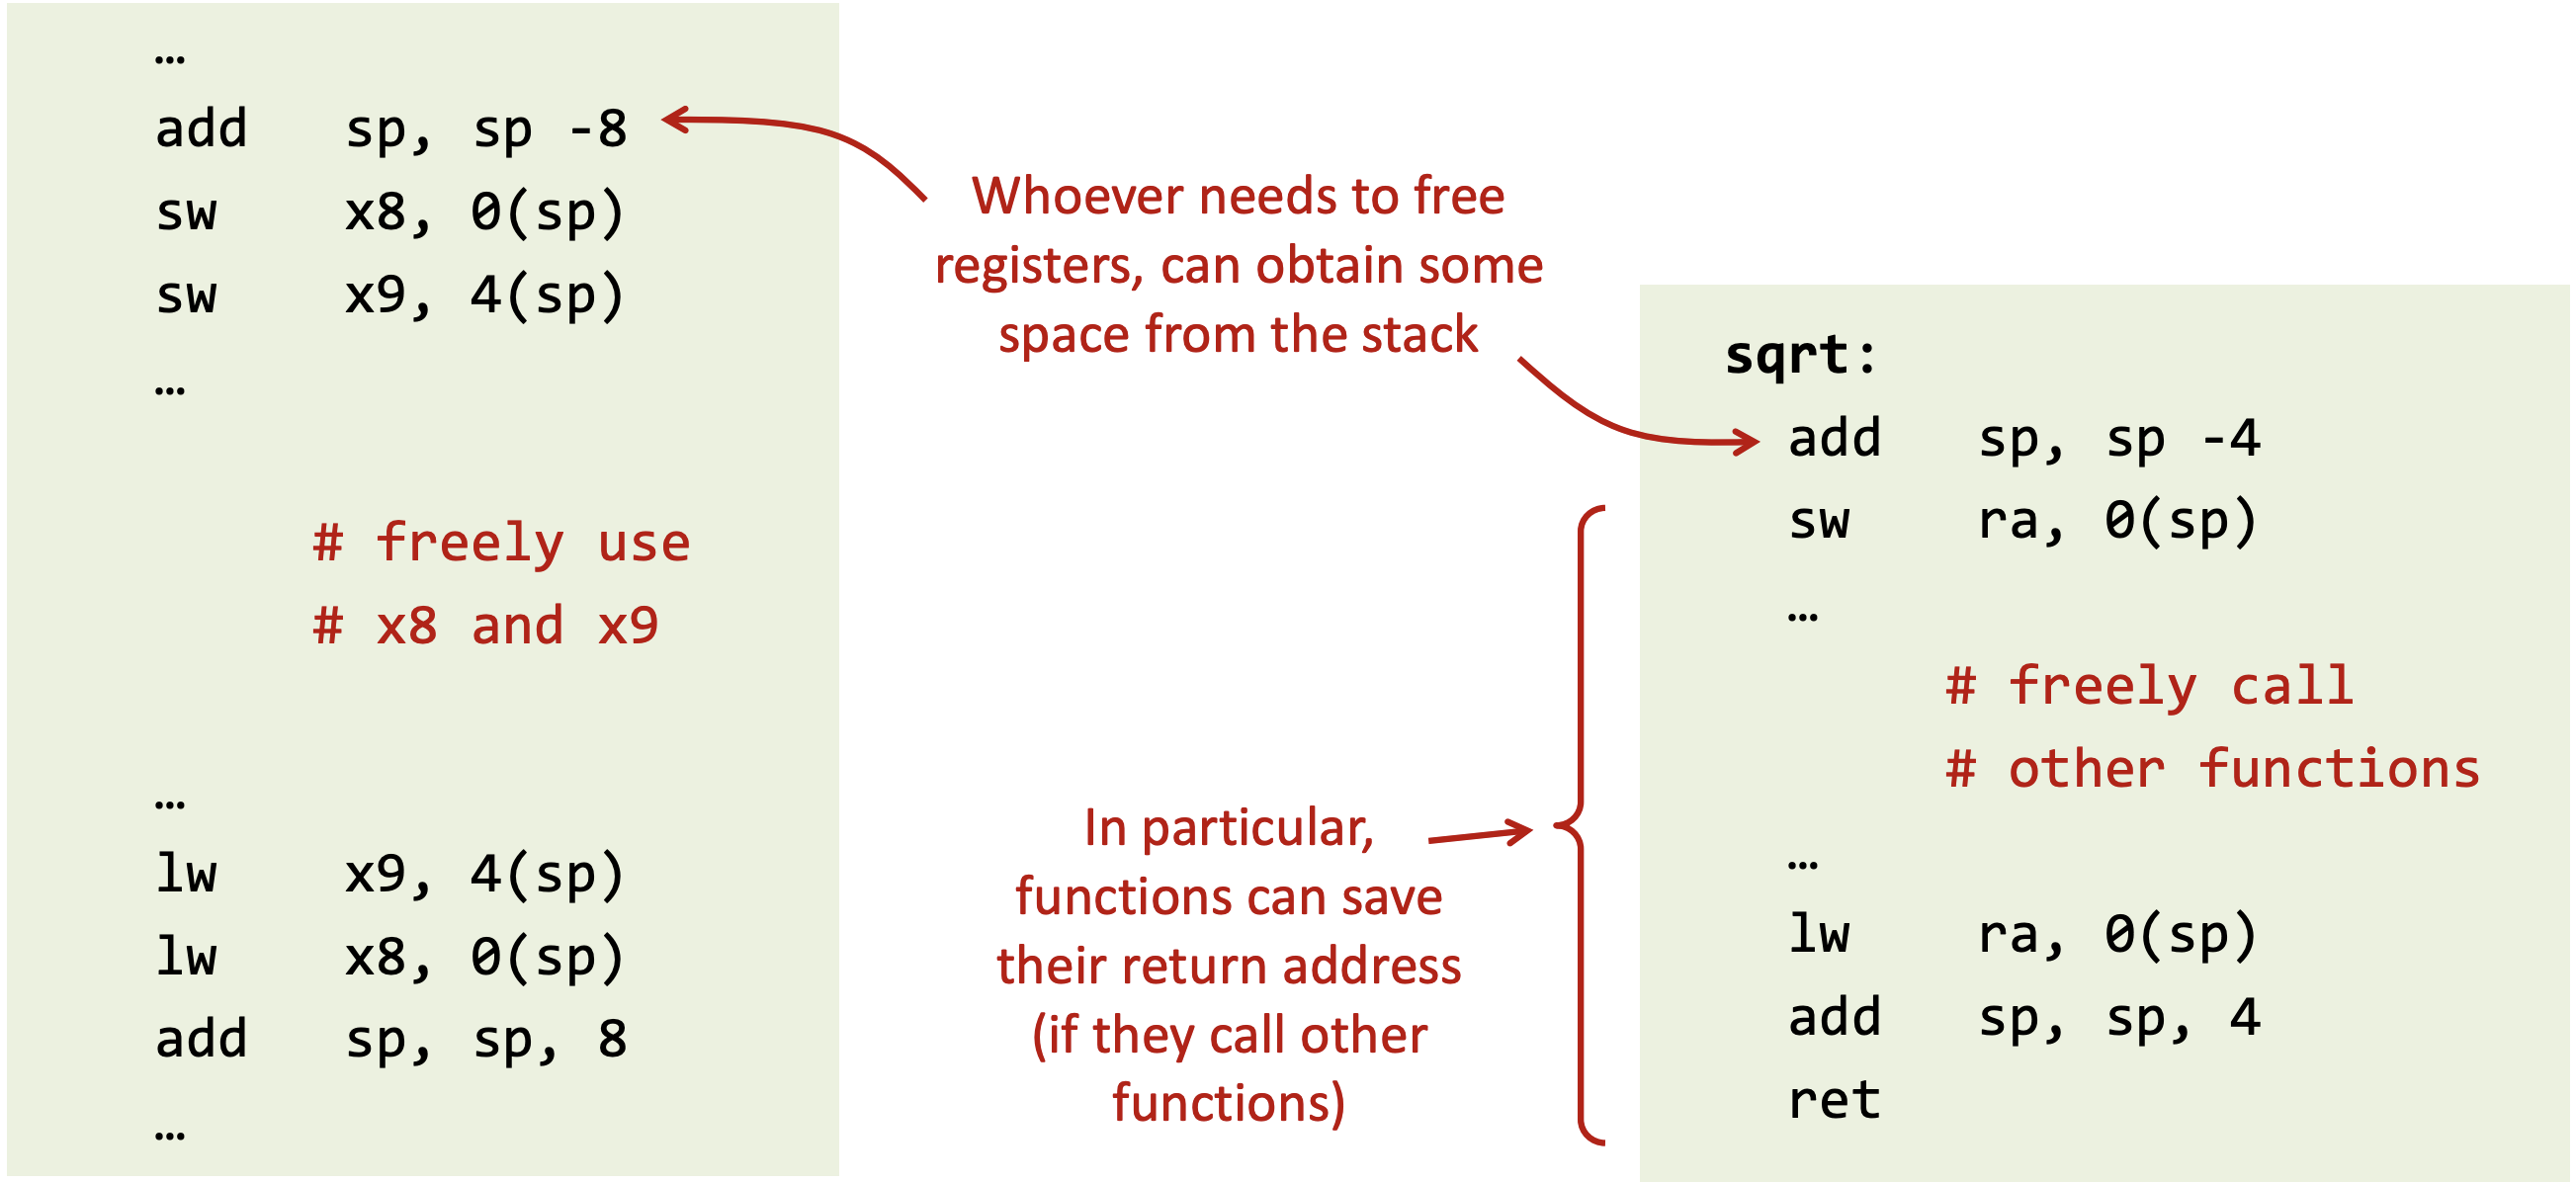
\includegraphics[width=0.75\textwidth]{chapters/chapter1b/images/spilling.png}
\end{center}

\subsection{Register across functions}
In assembly programming, handling registers across functions can be managed in two main ways: either functions \textbf{change registers} and expect the caller to save their values, or functions \textbf{preserve registers} and ensure that the register values remain the same across function calls.

\begin{itemize}
    \item On the left, the function \texttt{sqrt} changes the value of register \texttt{x20}, requiring the caller to save and restore its value.
    \item On the right, the function \texttt{sqrt} preserves the value of \texttt{x20}, ensuring that the caller does not need to manage the saving and restoring.
\end{itemize}

This distinction is important, but it does not cause issues as long as there is agreement on how registers are handled. \\
\textit{In case it's still not clear, we're looking at the \texttt{sw} instruction}

\begin{center}
    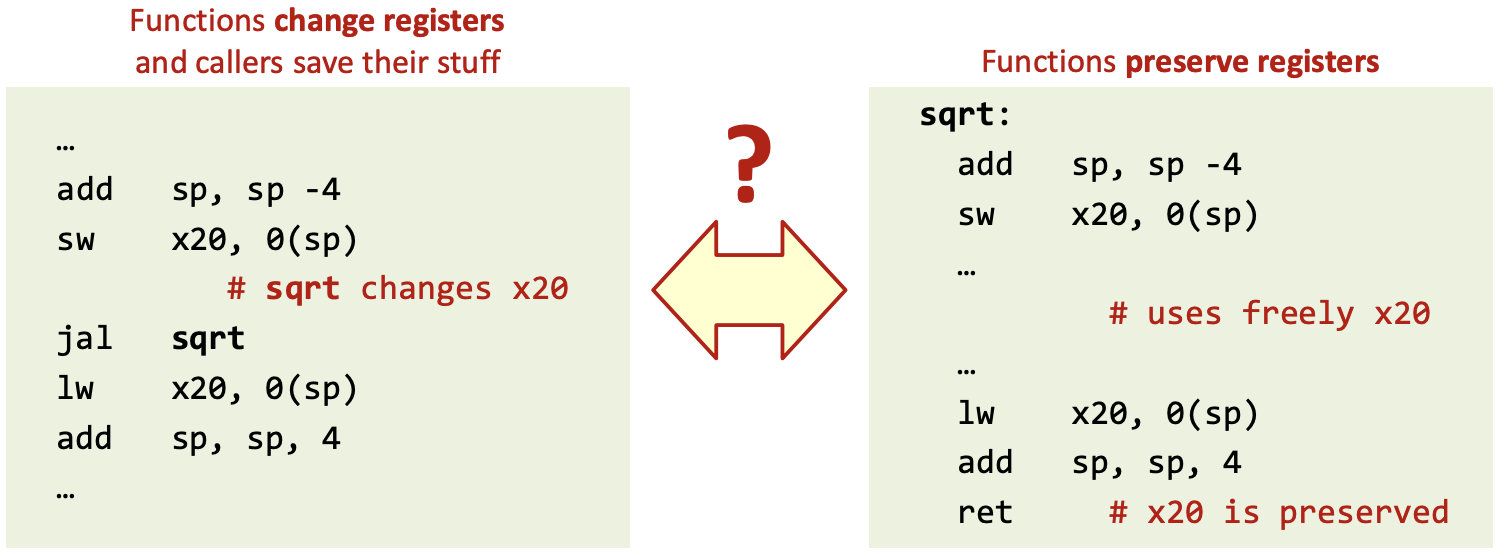
\includegraphics[width=0.7\textwidth]{chapters/chapter1b/images/registers.png}
\end{center}

\subsection{Preserving Registers}
In RISC-V, register preservation is managed through a combination of callee-saved and caller-saved registers. \\
Callee-saved registers (such as \texttt{s0}, \texttt{s1}, and \texttt{s2-11}) are preserved by the called function, ensuring that their values remain unchanged after the function call.  \\
Caller-saved registers (such as \texttt{t0}, \texttt{t1-2}, and \texttt{t3-6}) are temporary and do not need to be preserved by the called function, meaning the caller must save them if their values are important. \\
\begin{center}
    \begin{tabular}{|c|c|c|c|}
        \hline
        \textbf{Register} & \textbf{ABI Name} & \textbf{Description} & \textbf{Preserved across call?} \\ \hline
        x0  & zero  & Hard-wired zero                        & \textemdash    \\ \hline
        x1  & ra    & Return address                         & No             \\ \hline
        x2  & sp    & Stack pointer                          & Yes            \\ \hline
        x5  & t0    & Temporary/alternate link register      & No             \\ \hline
        x6--7 & t1--2 & Temporaries                          & No             \\ \hline
        x8  & s0/fp & Saved register/frame pointer           & Yes            \\ \hline
        x9  & s1    & Saved register                        & Yes            \\ \hline
        x18--27 & s2--11 & Saved registers                   & Yes            \\ \hline
        x28--31 & t3--6 & Temporaries                        & No             \\ \hline
        \end{tabular}
\end{center}

\section{Passing Arguments in RISC-V}

In RISC-V, there are two main ways to pass arguments to functions:

\subsection{Option 1: Using Registers}
- Specific registers are used to pass arguments and return results. \\
\vskip 0.1in
- This can be done in a straightforward way, where each function uses different registers (e.g., passing an argument in \texttt{x5} and returning the result in \texttt{x6}).
\vskip 0.1in
- A more structured approach is to follow a convention where arguments are passed in registers \texttt{x10} to \texttt{x17}, with results returned in \texttt{x10}.  \\
\vskip 0.1in
- The limitation: if there are more arguments than available registers (e.g., more than 8 arguments), this approach is insufficient.  \\

\subsection{Option 2: Using the Stack}
- When registers are not enough, extra arguments are placed on the stack.  \\
\vskip 0.1in
- The stack offers a universal solution because it has no practical limit on size.  \\
\vskip 0.1in
- However, using the stack is more complex and requires additional work compared to using registers.  \\

\subsection{The RISC-V Approach}
- RISC-V uses a combination of both methods.  \\
\vskip 0.1in
- Registers \texttt{x10} to \texttt{x17} are used to pass arguments, with \texttt{x10} and \texttt{x11} also handling return values. \\
\vskip 0.1in
- If more arguments are needed beyond what these registers can handle, they are passed via the stack. 

\begin{center}
    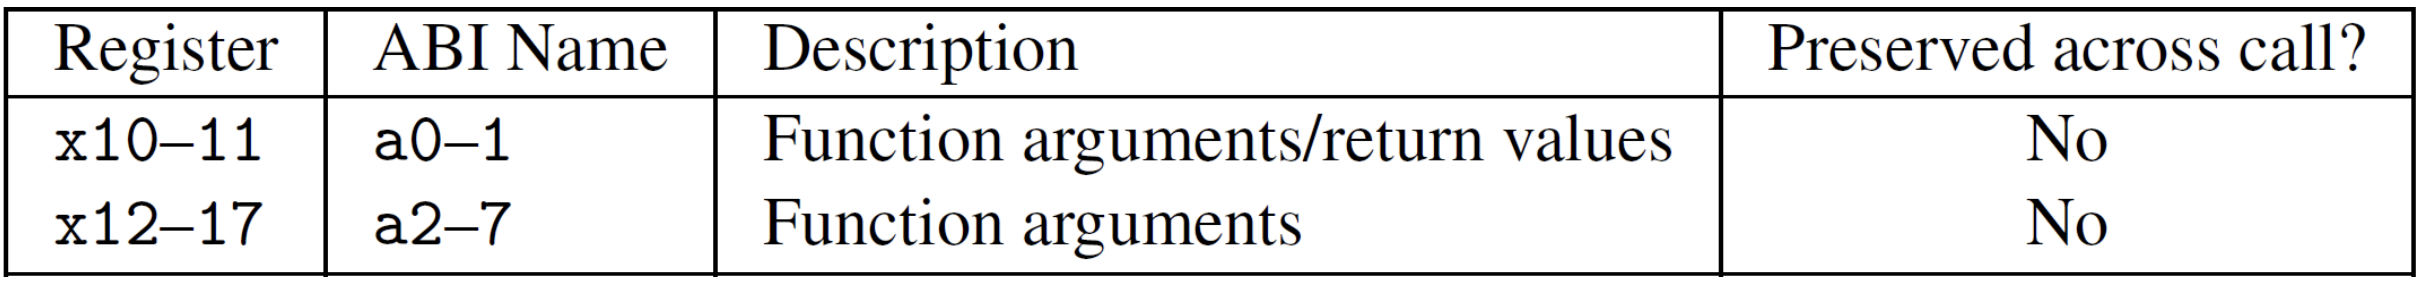
\includegraphics[width=0.75\textwidth]{chapters/chapter1b/images/arguments.png}
\end{center}
\textit{Register reserved for arguments and return values in RISC-V.}

\section{Summary of RISC-V Register Conventions}
\begin{center}
    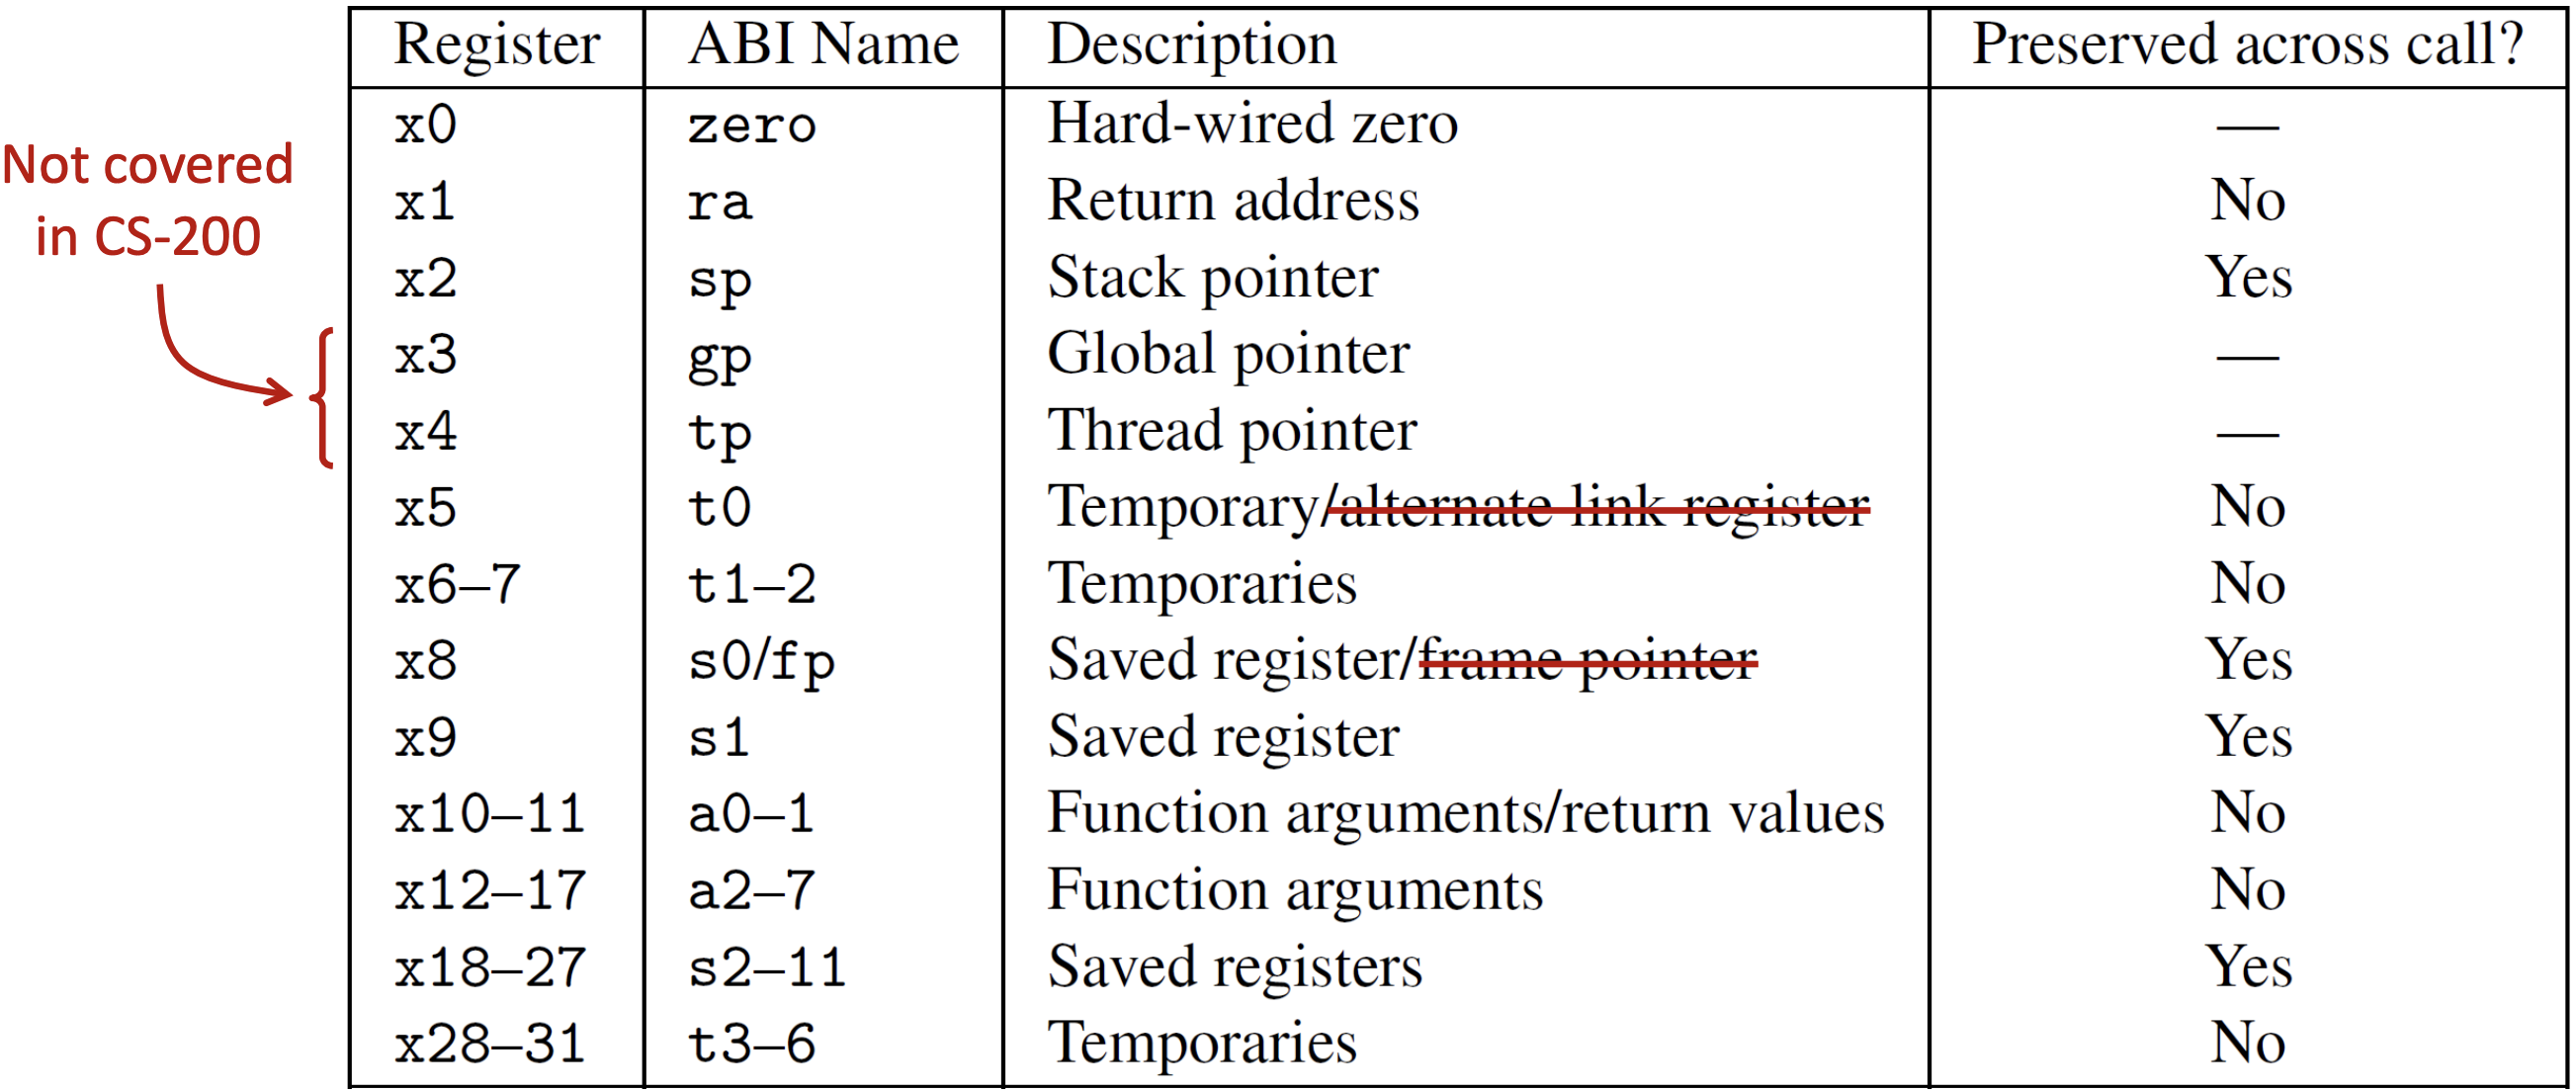
\includegraphics[width=0.75\textwidth]{chapters/chapter1b/images/summary.png}
\end{center} % Including chapter0.tex from chapters folder
\chapter{Part I(c) - ISA Memory and Addressing Modes - W 2.1}

\section{Memory}
\textit{Memory is a really important component of a computing system, we store our programs in it, we store our data in it, and it's through memory that we receive and send data.} \\ \vspace*{5px}
\textbf{Though memory is very useful it has three main drawbacks:} \\ \vspace*{5px}
\begin{itemize}
    \item[-] It's \textbf{slow} $\rightarrow$ Caches 
    \item[-] It's \textbf{finite} $\rightarrow$ Virtual Memory
    \item[-] It can make an ISA \textbf{too complex} $\rightarrow$ Pipelining
\end{itemize}
\textit{no worries we'll cover each one of these in this chapter.}

\subsection{Address and Data}
\textit{Data in Memory can be accessed by an adress, meaning i's a \textit{Random Access} (it can access a memory value without going through the preceding ones).} \\ \vspace*{5px}
\textit{Professor Remark: "There's not anything random about this memory, we'd better call it and abitrary access memory. (!not and official  name)"} \\ \vspace*{5px}
\vspace*{5px}
\begin{minipage}[htp]{0.45\textwidth}
\begin{center}
    \begin{tabular}{|c|c|}
    \hline
    \textbf{Address} & \textbf{Value} \\
    \hline
    \texttt{0} & 12 \\ 
    \hline
    \texttt{1} & 6 \\ 
    \hline
    \texttt{2} & 4 \\ 
    \hline
    \texttt{3} & 1 \\ 
    \hline
    \texttt{4} & 0 \\ 
    \hline
    \texttt{5} & 3 \\ 
    \hline
    \texttt{6} & 1 \\ 
    \hline
    \texttt{7} & 13 \\ 
    \hline
    \texttt{8} & 15 \\ 
    \hline
    \texttt{9} & 9 \\ 
    \hline
    \texttt{10} & 3 \\ 
    \hline
    \texttt{11} & 5 \\ 
    \hline
    \texttt{12} & 0 \\ 
    \hline
    \texttt{13} & 0 \\ 
    \hline
    \texttt{14} & 0 \\ 
    \hline
    \texttt{15} & 0 \\ 
    \hline
    \end{tabular}
\end{center}
\end{minipage}
\hfill
\vline
\hfill
\begin{minipage}[htp]{0.45\textwidth}
\begin{center}
    \begin{tabular}{|c|c|}
    \hline
    \textbf{Write} & \textbf{Read} \\ 
    \hline
    \texttt{\textbf{Memory[5] = 3}} & \texttt{Memory[5]?} \\ 
    \hline
    \end{tabular}
\end{center}
\end{minipage}

\section{Many Types of Memories}
We may distinguish between different types of memories based on their \textbf{technology}, such as SRAM, DRAM, EPROM, and Flash, and their \textbf{capabilities}, including \textbf{speed}, \textbf{capacity}, \textbf{density}, \textbf{writability} (whether they are writable, permanent, or reprogrammable), as well as their \textbf{size}, \textbf{volatility}, and \textbf{cost}. \\ \vspace*{5px}
\subsection{Functional Taxonomy of Memories}
\begin{center} 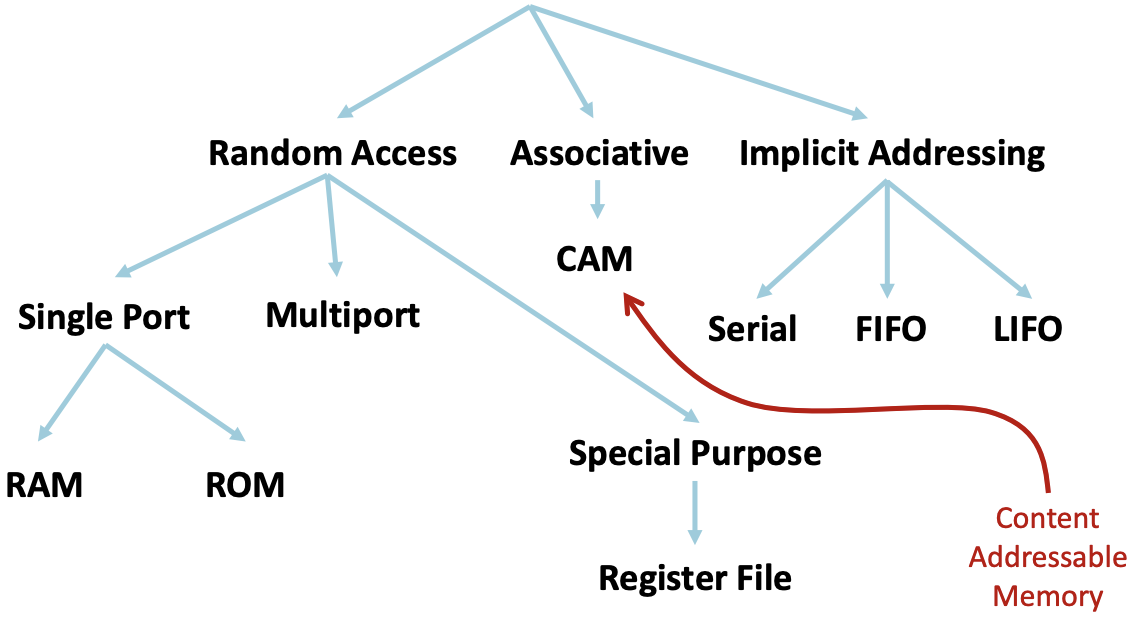
\includegraphics[width=0.45\textwidth]{chapters/chapter1c/images/funct_tax.png} \end{center}
\begin{itemize}
    \item[] \textbf{Multiport} memory allows simultaneous access by multiple processors, while \textbf{single-port} memory supports only one at a time.
    \item[] \textbf{Non-Random Access memories}
    \begin{itemize}
        \item \textbf{Adsociative} memories enable fast data retrieval by content rather than address, making it useful for cache memory, pattern recognition, and efficient lookups in large datasets.
        \item In \textbf{Implicit addressing} the address of the data to be operated on is inferred directly by the operation code (opcode), without explicitly specifying the address in the instruction.
    \end{itemize}
\end{itemize}


\subsection{Taxonomy of Random Access Memories}
\begin{center}
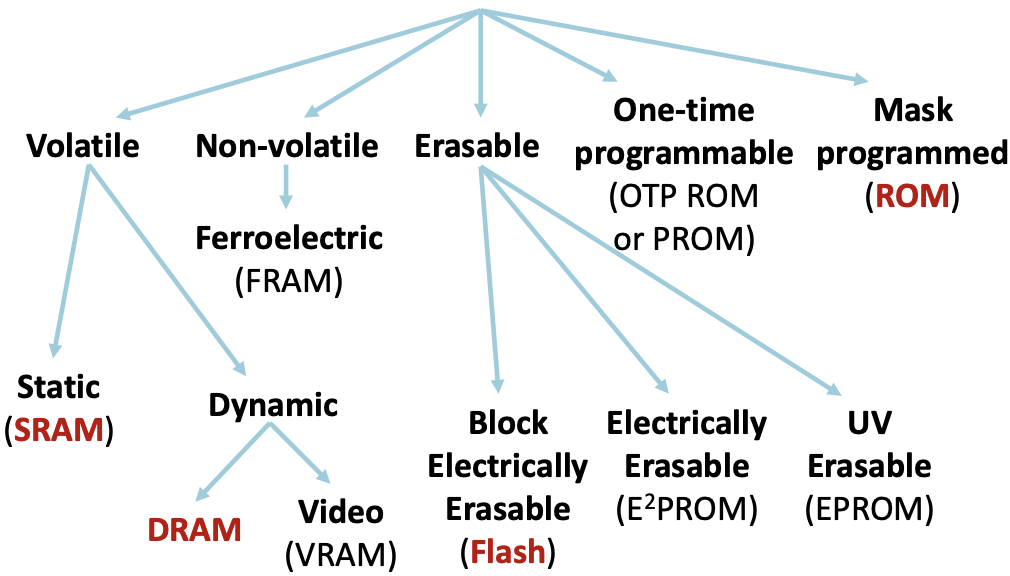
\includegraphics[width=0.45\textwidth]{chapters/chapter1c/images/ram_tax.png}
\end{center}
\newpage
\subsection{Basic Structure}
\textit{Remember, a Data Flip Flop, stores a 1 bit value by updating the output value to the input value at the rising edge of the clock signal.} \\ \vspace*{5px}
\begin{minipage}[htp]{0.35\textwidth} 
\begin{center}
    \begin{tabular}{|c|c|}
        \hline
        \textbf{Address} & \textbf{Value} \\ 
        \hline
        \texttt{0} & 12 \\ 
        \hline
        \texttt{1} & 6 \\ 
        \hline
        \texttt{2} & 4 \\ 
        \hline
        \texttt{3} & 1 \\ 
        \hline
        \texttt{4} & 0 \\ 
        \hline
        \texttt{5} & 3 \\ 
        \hline
        \texttt{6} & 1 \\ 
        \hline
        \texttt{7} & 13 \\ 
        \hline
        \texttt{8} & 15 \\ 
        \hline
        \texttt{9} & 9 \\ 
        \hline
        \texttt{10} & 3 \\ 
        \hline
        \texttt{11} & 5 \\ 
        \hline
        \texttt{12} & 0 \\ 
        \hline
        \texttt{13} & 0 \\ 
        \hline
        \texttt{14} & 0 \\ 
        \hline
        \texttt{15} & 0 \\ 
        \hline
        \end{tabular}
\end{center}
\end{minipage}
\hfill
\vline
\hfill
\begin{minipage}[htp]{0.35\textwidth}
\textbf{16 x 4 Memory Cells (~Special DFFs (Data Flip-Flops))} \\
\begin{center}
    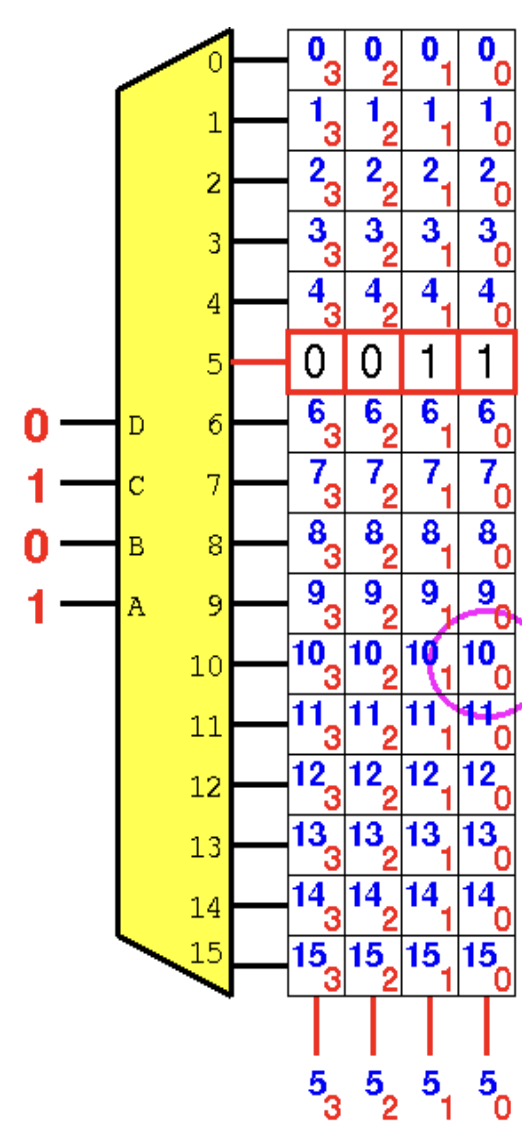
\includegraphics[width=0.45\textwidth]{chapters/chapter1c/images/structure.png}
\end{center}
\end{minipage} \\
\vfill
\begin{minipage}[htp]{0.45\textwidth}   
    \subsection{Write Operations}
    \textit{The D is connected to the Data outside of the system and at the risiing edge it updates the value of the DFF.} \textbf{The AND gate ensures that the write signal is high when the clock signal is high.} \\ \vspace*{5px}
    \begin{center}
        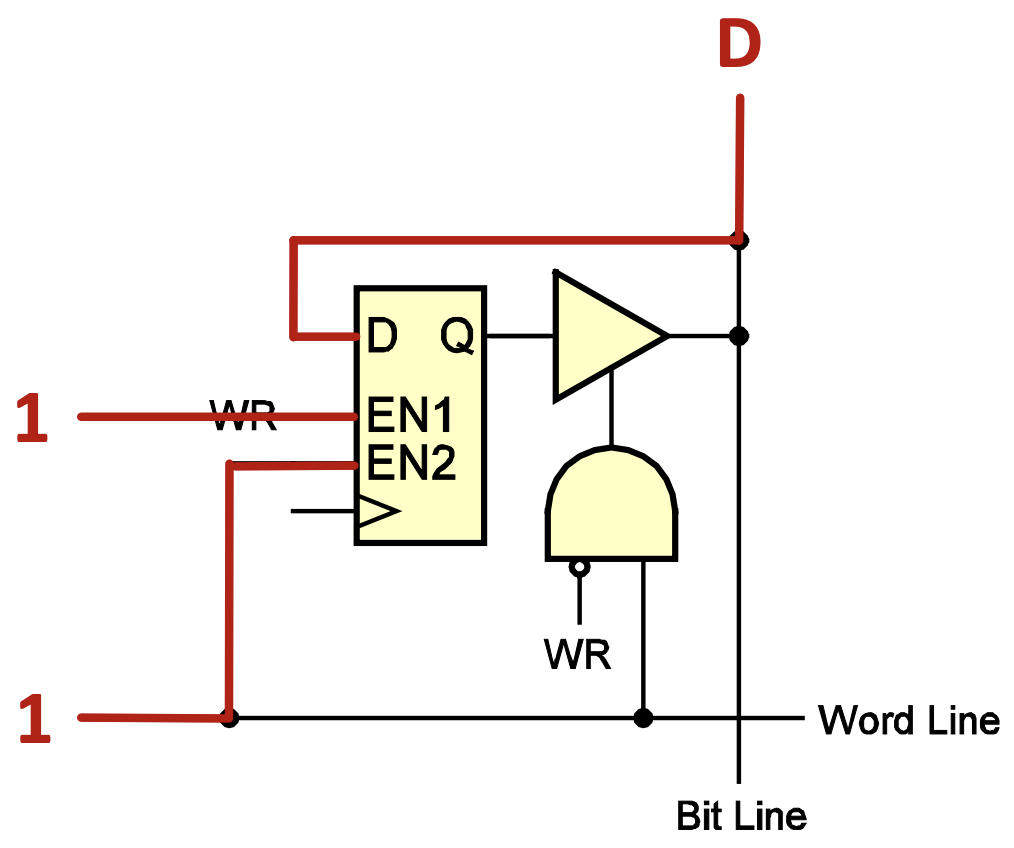
\includegraphics[width=0.45\textwidth]{chapters/chapter1c/images/write.png}
    \end{center}
\end{minipage}
\hfill  
\vline
\hfill
\begin{minipage}[htp]{0.45\textwidth}
    \subsection{Read Operations}
    \textit{D is still connected to the Data, remember the tri-state driver is active when it's enable signal is active (so when the wr is off and the operation signal is sent.).} \\ \vspace*{5px}
    \begin{center}
        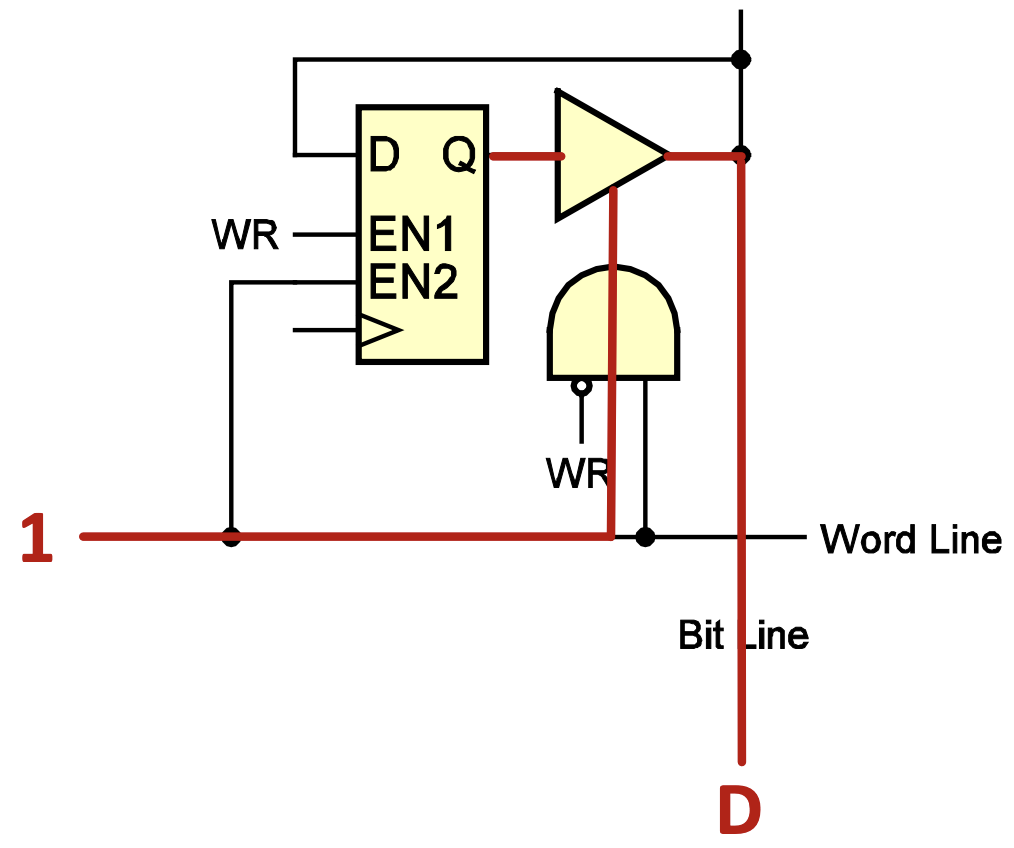
\includegraphics[width=0.45\textwidth]{chapters/chapter1c/images/read.png}
    \end{center}
\end{minipage}

\vspace*{5px}
\subsection{Practical SRAMs}
\textbf{DISCLAIMER !!: Combinational loops are prohibited as they can lead to unstable behavior, unpredictable timing, simulation and synthesis issues, excessive power consumption, and lack of a defined reset state, making them unsuitable for reliable digital circuit design.} \\ \vspace*{5px}
\textit{While the type of memory we've juste seen is small, and very fast, SRAM memories uses 6 transitors per cell (less than the previous design). We've also seen (in Taxonomy) that SRAM is \textbf{static} meaning it doesn't require periodic refresh.} \\ \vspace*{5px}
\begin{minipage}[htp]{0.45\textwidth} 
    \begin{center}
        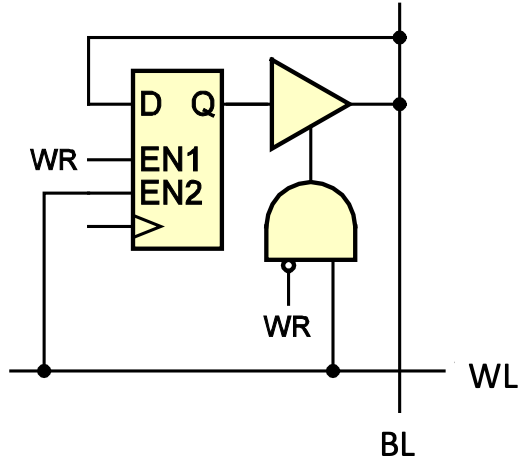
\includegraphics[width=0.55\textwidth]{chapters/chapter1c/images/ram.png}
    \end{center}
    \end{minipage}
    \hfill
    \vline
    \hfill
    \begin{minipage}[htp]{0.45\textwidth}
    \begin{center}
        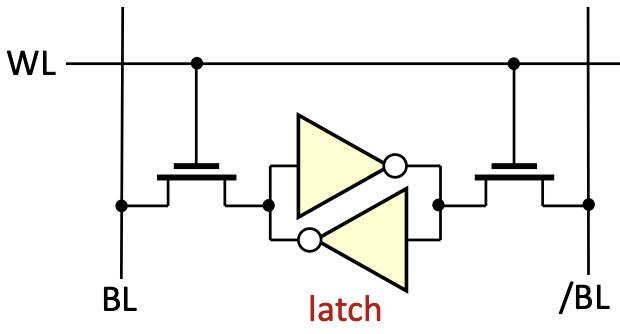
\includegraphics[width=0.55\textwidth]{chapters/chapter1c/images/sram.png}
    \end{center}
    \end{minipage}

\subsection{DRAMs}
\textit{Dynamic RAMS(DRAMs) are the densest and cheapest type of RAM memory, it stores information as charge in small capacitors. This makes the DRAM need periodic refresh otherwise the charge might leak off (~60ms) the capacitor due to parasitic resistances and the information lost} \\ \vspace*{5px}

\begin{minipage}[htp]{0.45\textwidth}
    \textbf{Refresh means, we come back before the end of a charge (~60ms) and we rewrite the value, if there is still some charge, we add charge, if there's no charge and we keep as is.} \\ \vspace*{5px}
    \textit{Personal Remark: Dynamic = Bad, data dissapears and needs refresh}
\end{minipage}
\hfill
\vline  
\hfill
\begin{minipage}[htp]{0.45\textwidth}
    \begin{center}
        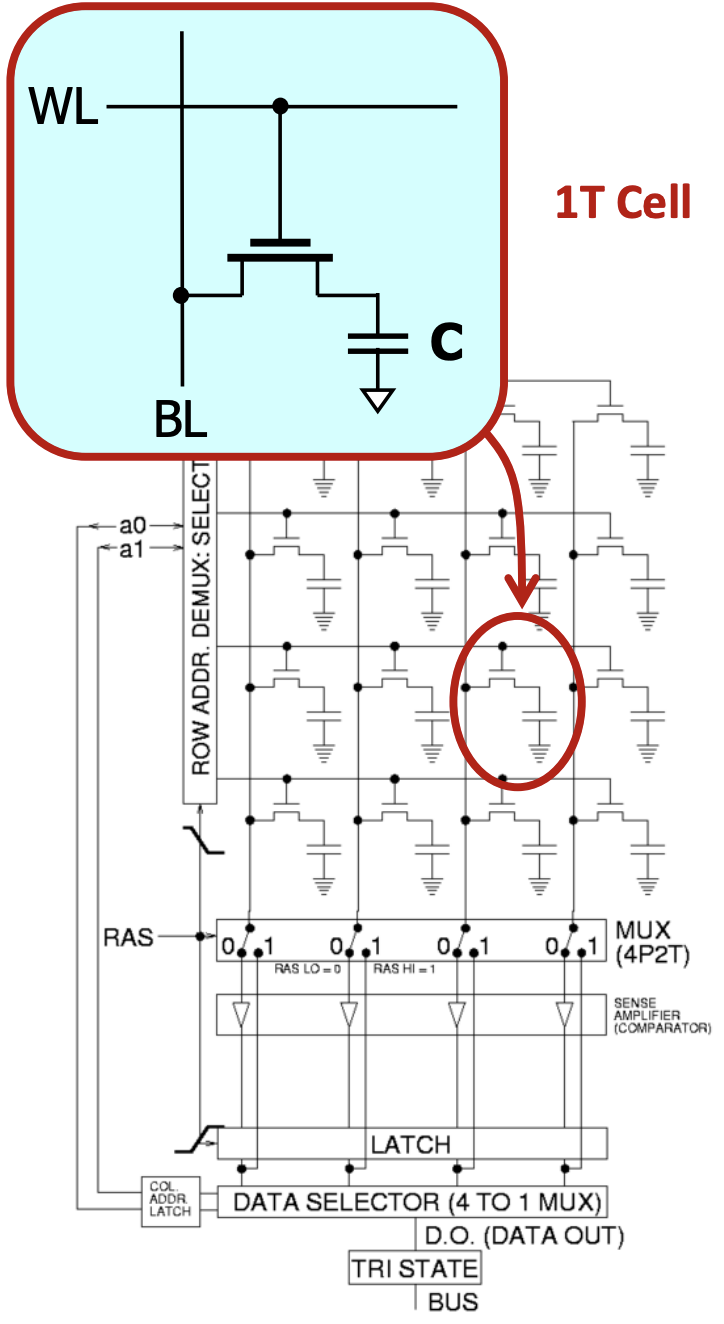
\includegraphics[width=0.5\textwidth]{chapters/chapter1c/images/dram.png}  
    \end{center}
\end{minipage}

\subsection{Ideal Random Access Memory}
\textit{A memory array uses an \(n\)-to-\(2^n\) decoder to select a word line based on the input address, enabling data to be read or written through the bit lines.}
\begin{center}
    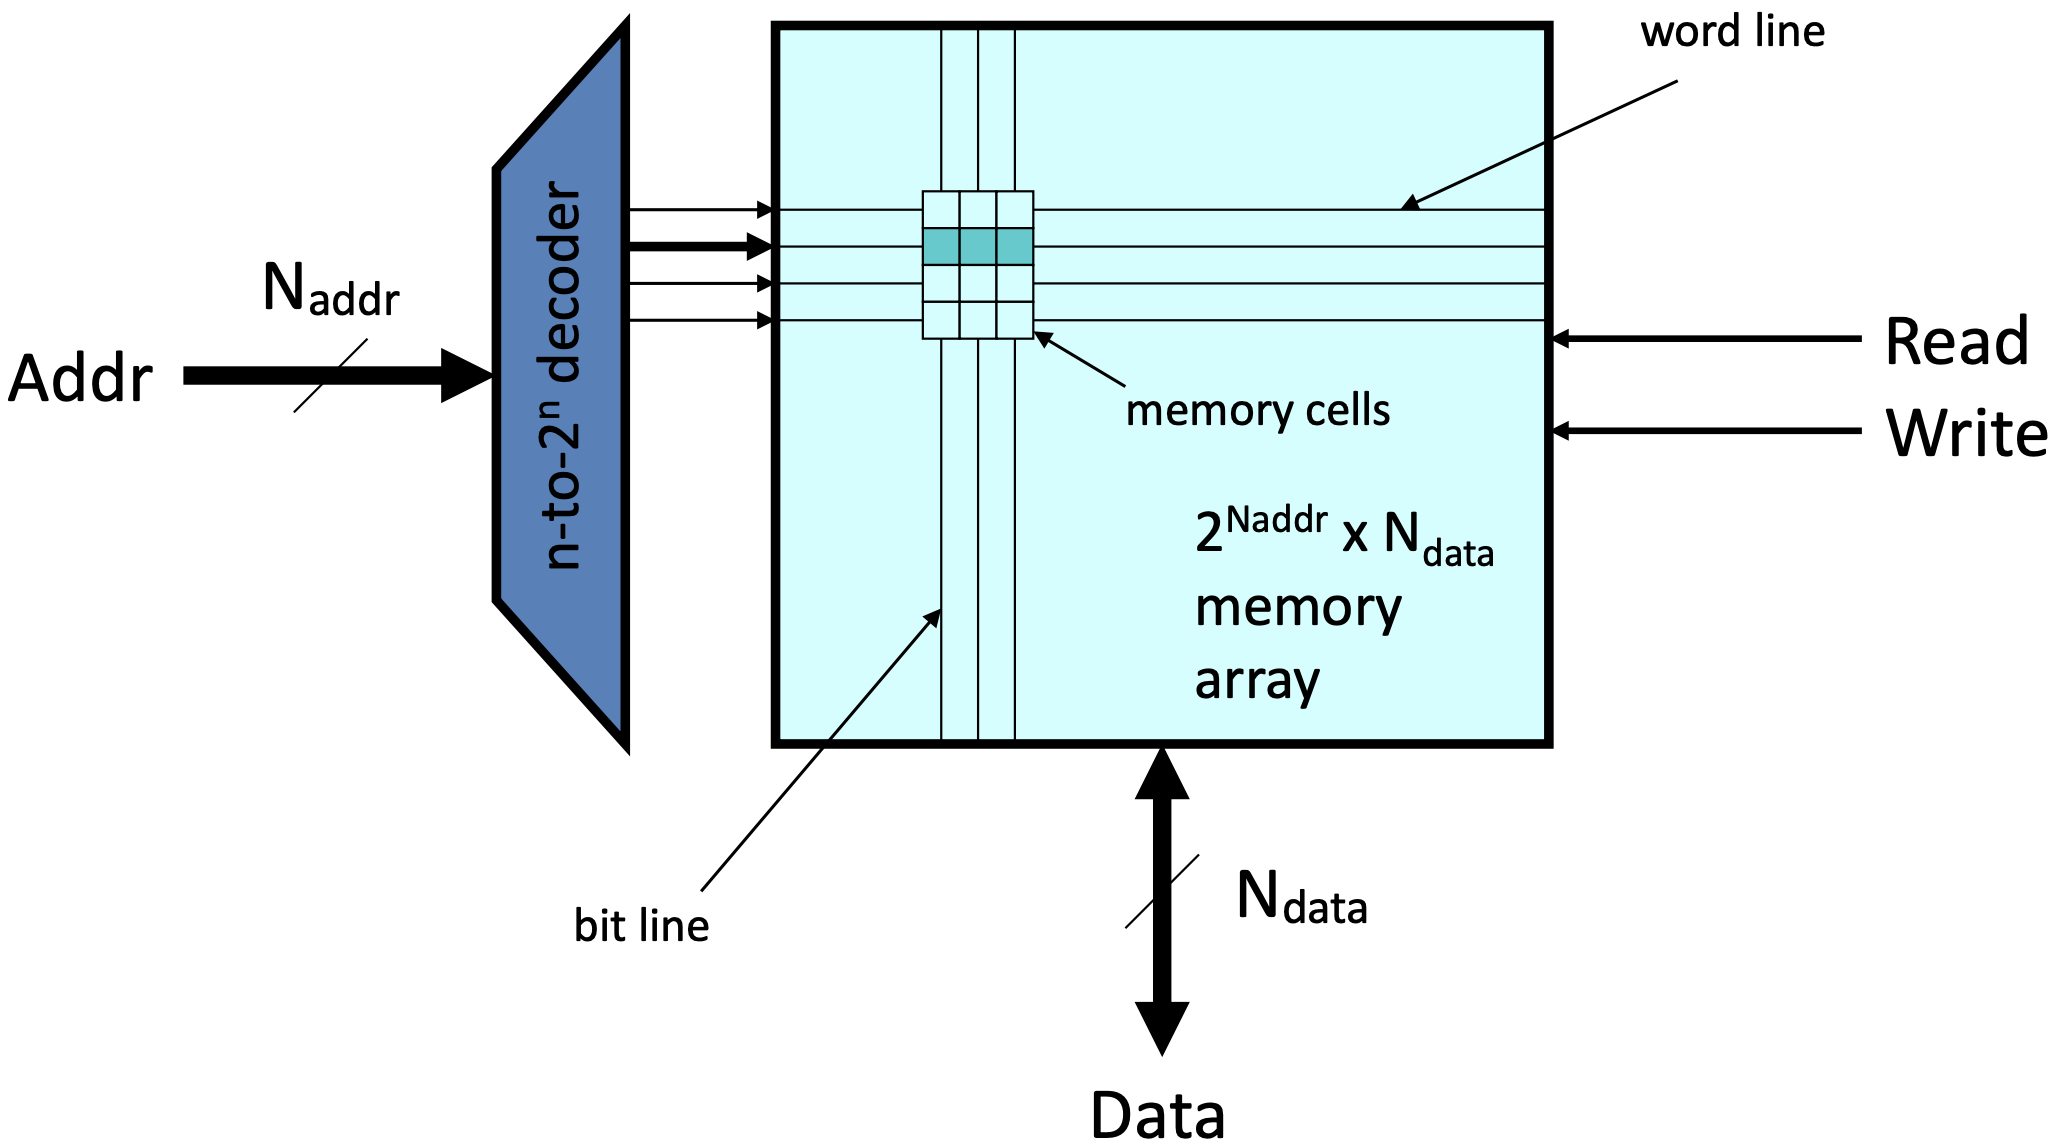
\includegraphics[width=0.45\textwidth]{chapters/chapter1c/images/ideal_ram.png}
\end{center}
\subsection{Physical Organisation }
\begin{center}
    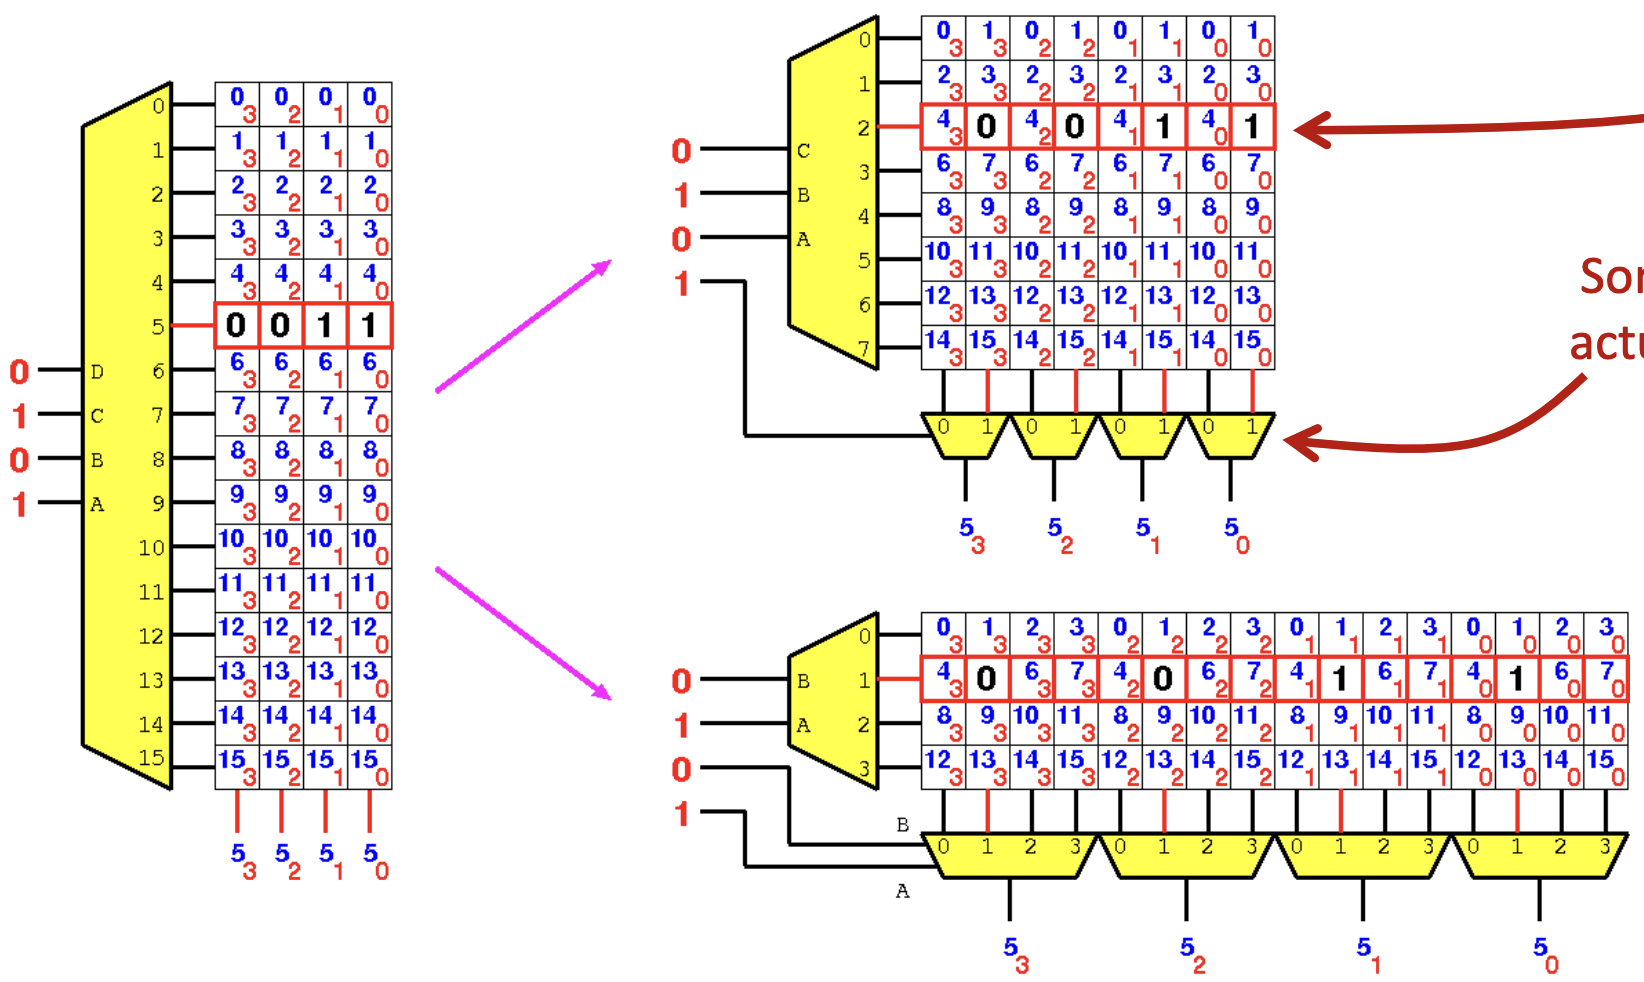
\includegraphics[width=0.45\textwidth]{chapters/chapter1c/images/organisation.png}
\end{center}
\textit{Out of all physical organizations, the squared one is the best one as it has the best performance. This layout facilitates faster access times and simplified wiring, resulting in improved computational efficiency and system scalability.}
\subsection{Realistic ROM Array}
\textit{ROMs are Read-Only Memories, they are used to store the program of the computer, they are non-volatile and can't be written to.} \\ \vspace*{5px}
\begin{center}
    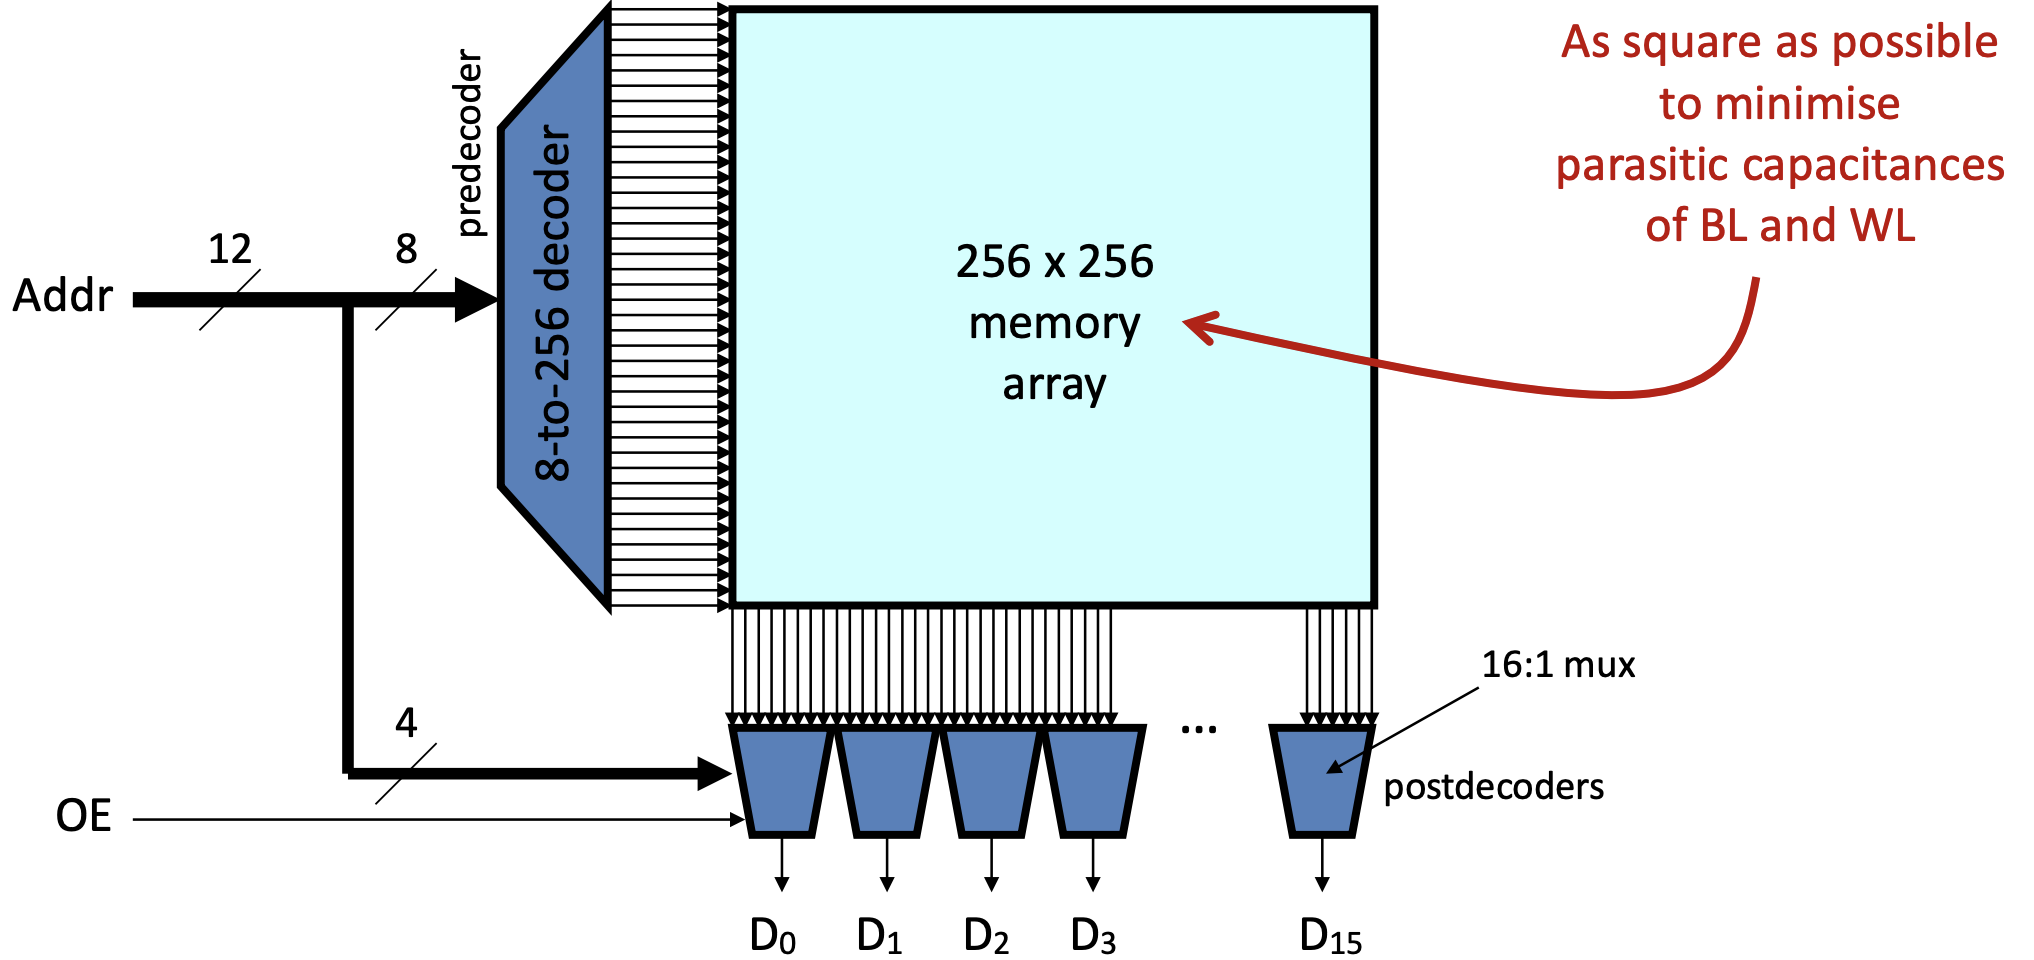
\includegraphics[width=0.45\textwidth]{chapters/chapter1c/images/rom.png}
\end{center}

\subsection{Static Ram Typical Interface}
\textit{This a typical interface of a SRAM, it has a 16-bit data input/output, a 16-bit address input, a write enable signal, and a circuit select signal.}
\begin{center}
    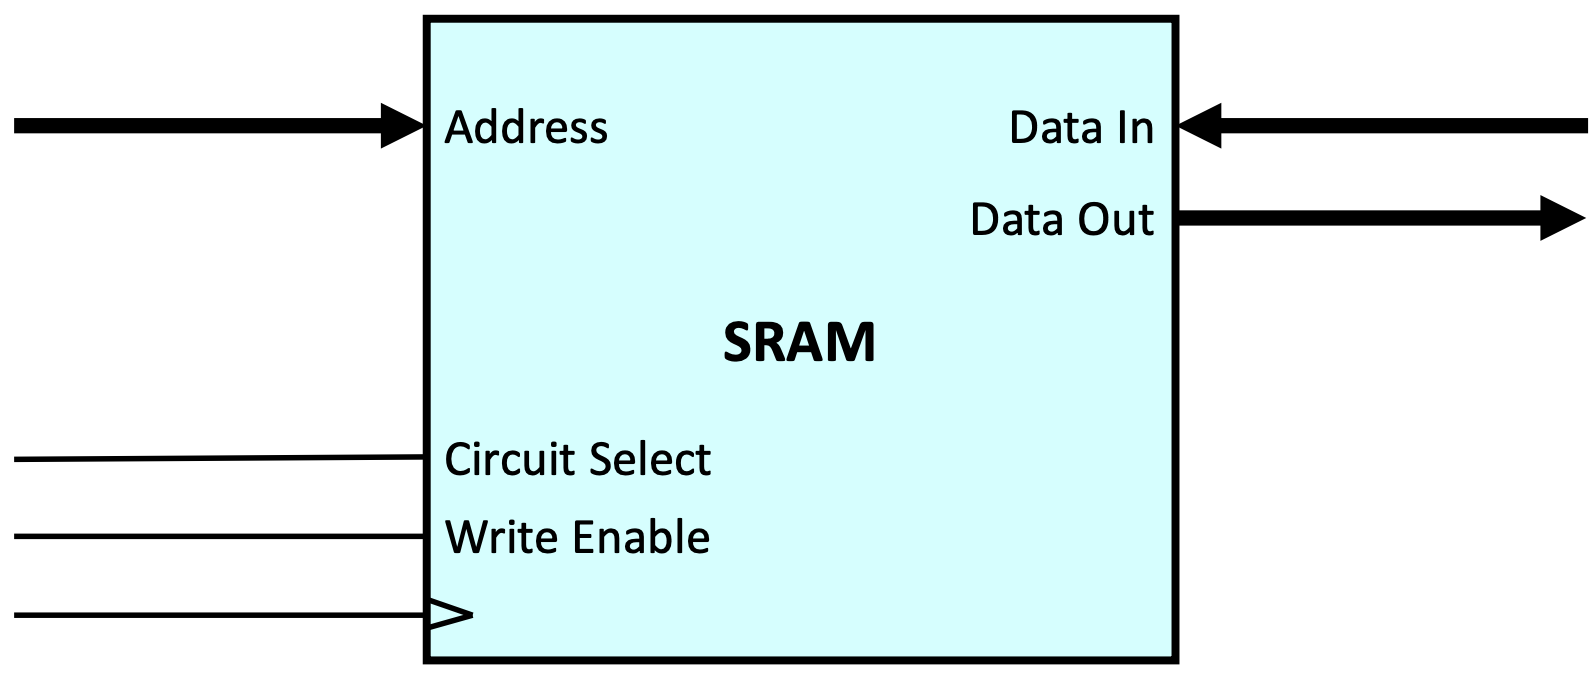
\includegraphics[width=0.45\textwidth]{chapters/chapter1c/images/sram_interface.png}
\end{center}

\section{Typical Asynchronous SRAM Read Cycle}
\textit{The read cycle of an asynchronous SRAM is initiated by the address input, which is decoded to select the word line, enabling the data to be read from the memory array and output to the data bus.} \\ \vspace*{5px}
\textit{Here, Tcyc is the cycle time, Tacc is the access time, and Ten is the enable time.}

\begin{minipage}[htp]{0.45\textwidth}
    \begin{center}
        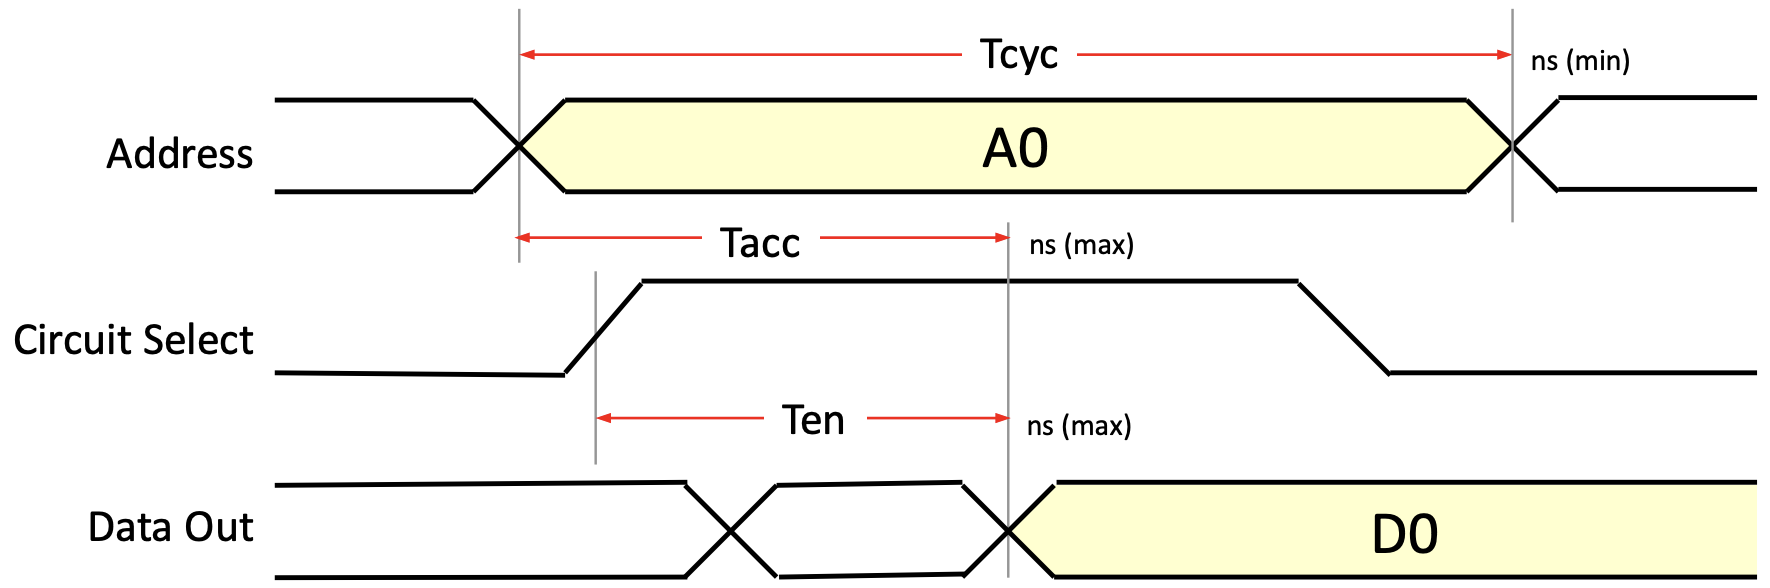
\includegraphics[width=0.45\textwidth]{chapters/chapter1c/images/sram_read.png}
    \end{center}
\end{minipage}
\hfill
\vline
\hfill
\begin{minipage}[htp]{0.45\textwidth}
    \begin{center}
        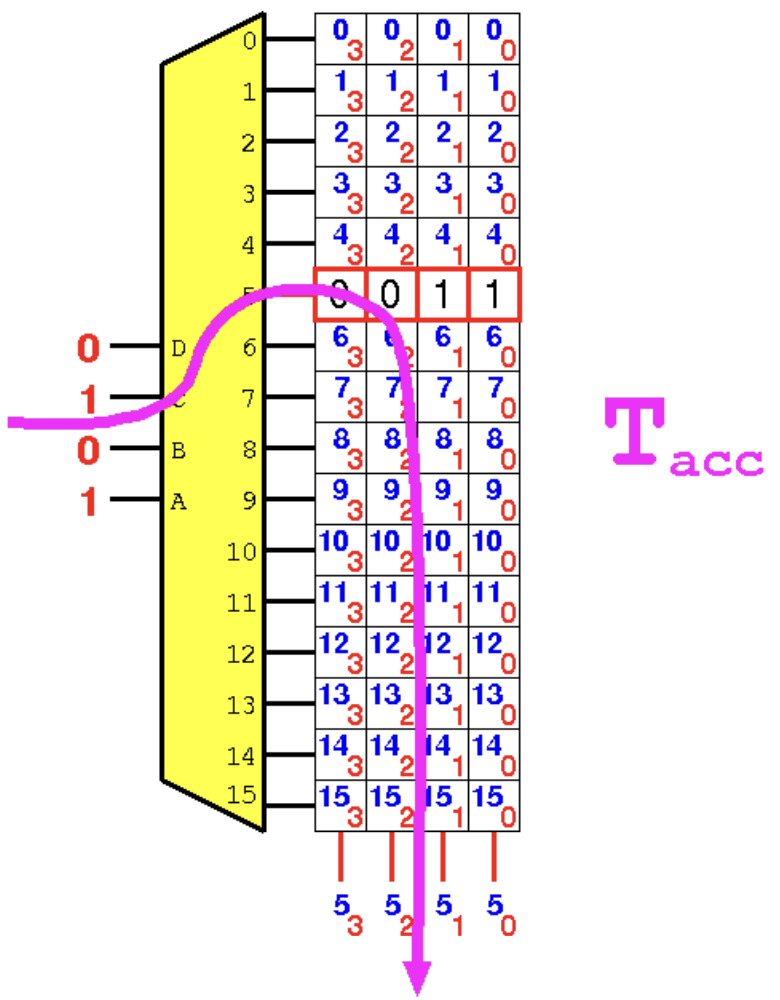
\includegraphics[width=0.45\textwidth]{chapters/chapter1c/images/sram_read2.png}
    \end{center}
\end{minipage}  

\subsubsection{Read Cycle}
\textit{Latency} defined as the number of cycles between the address asserted and data available \\ \vspace*{5px}
\begin{center}
    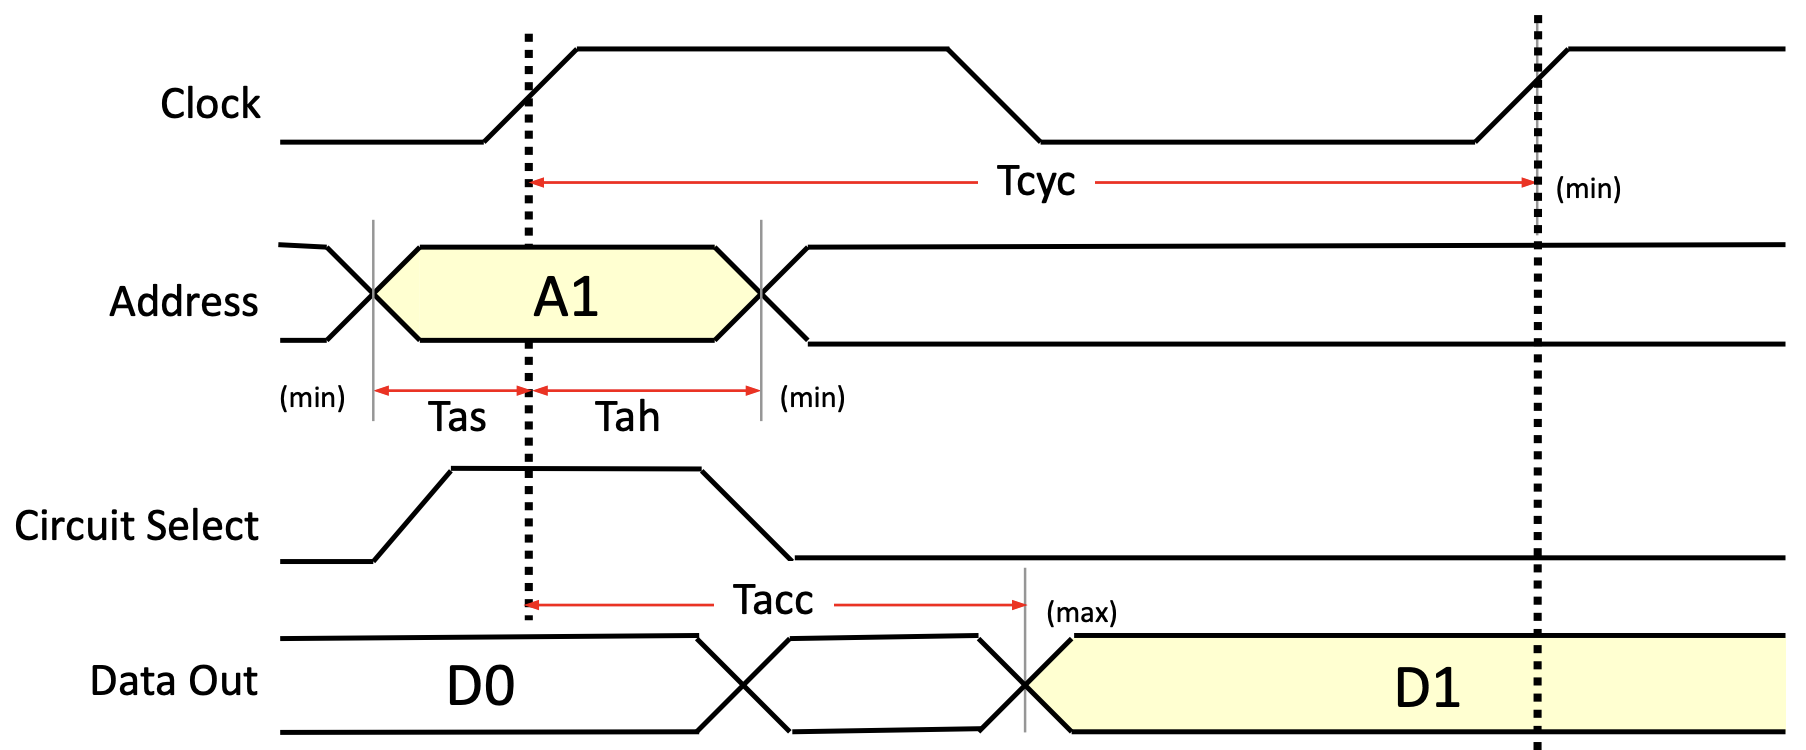
\includegraphics[width=0.45\textwidth]{chapters/chapter1c/images/read_cycle.png}
\end{center}
\subsubsection{Write Cycle}
\textit{Writes on the edge of the clock signal, as a DFF} \\ \vspace*{5px}
\begin{center}
    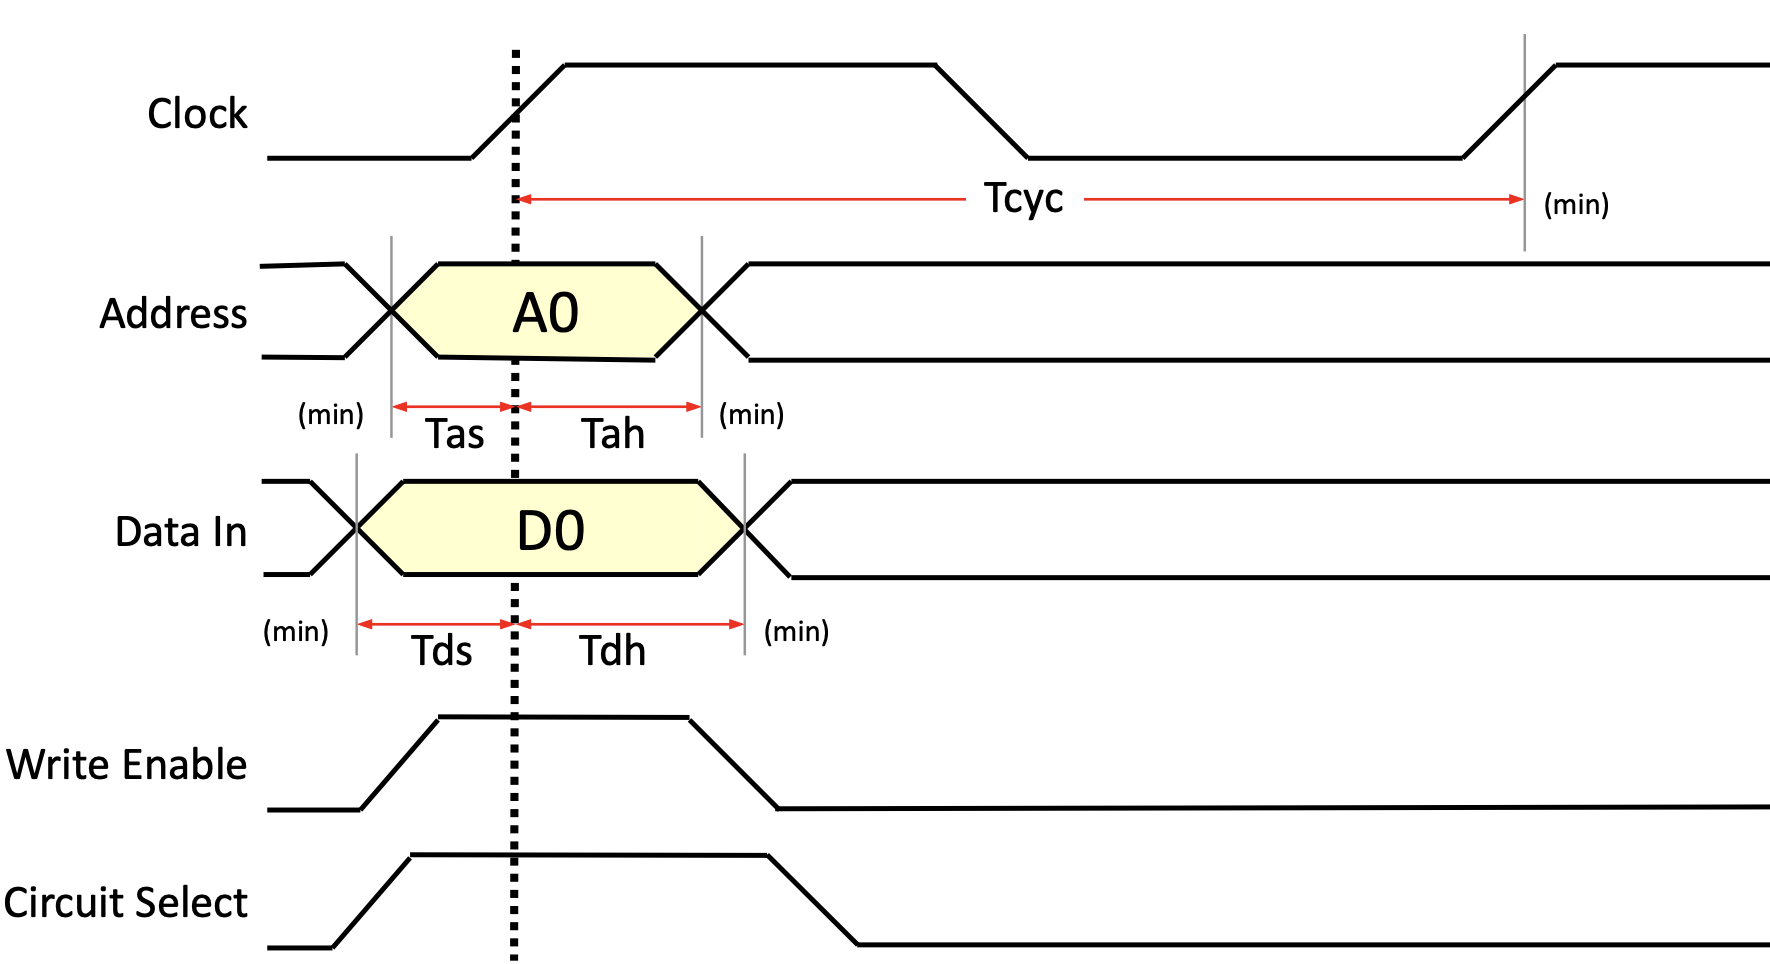
\includegraphics[width=0.45\textwidth]{chapters/chapter1c/images/write_cycle.png}
\end{center}


\section{Where is Memory in the Processor?}
\textit{In the processor we have memory in the Data memory component and in the Instruction memory component.} \\ \vspace*{5px}
\begin{center}
    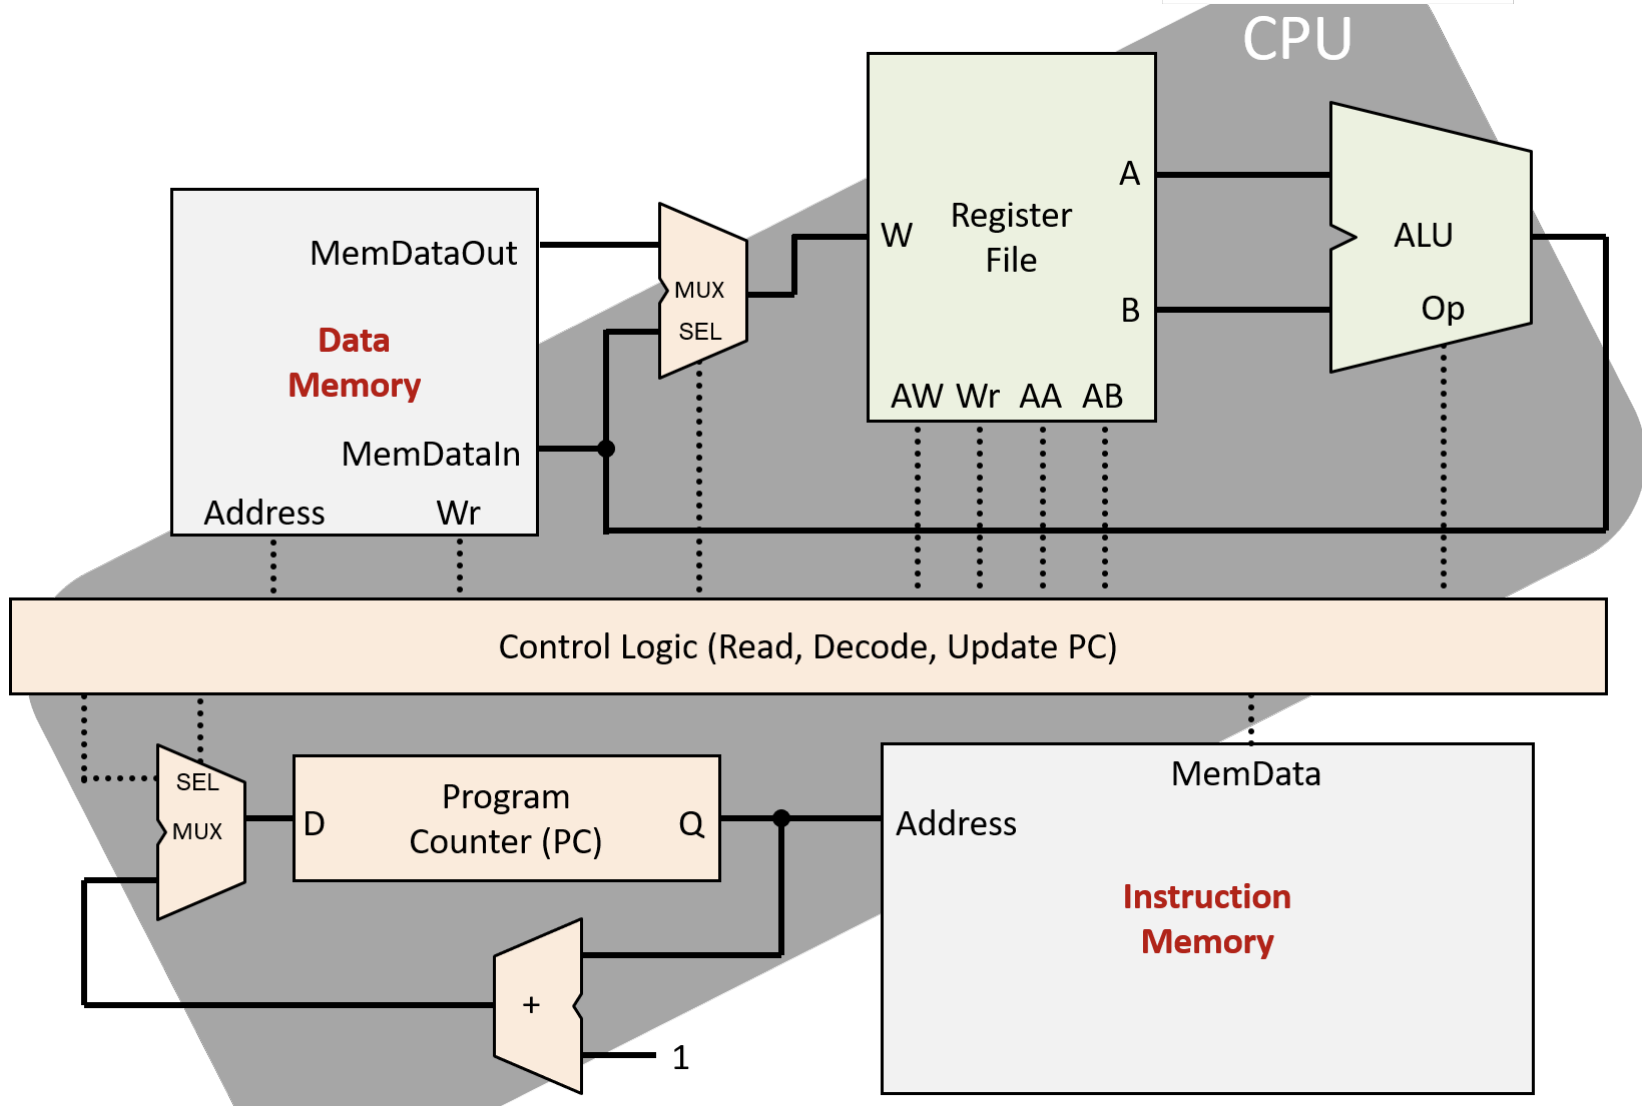
\includegraphics[width=0.45\textwidth]{chapters/chapter1c/images/processor.png}
\end{center}
\subsection{Arithmetic and Logic Instructions}
\textit{The register file can only contain a limited number of registers making it difficult to handle more complex computations and managing data input/output efficiently.}
\begin{center}
    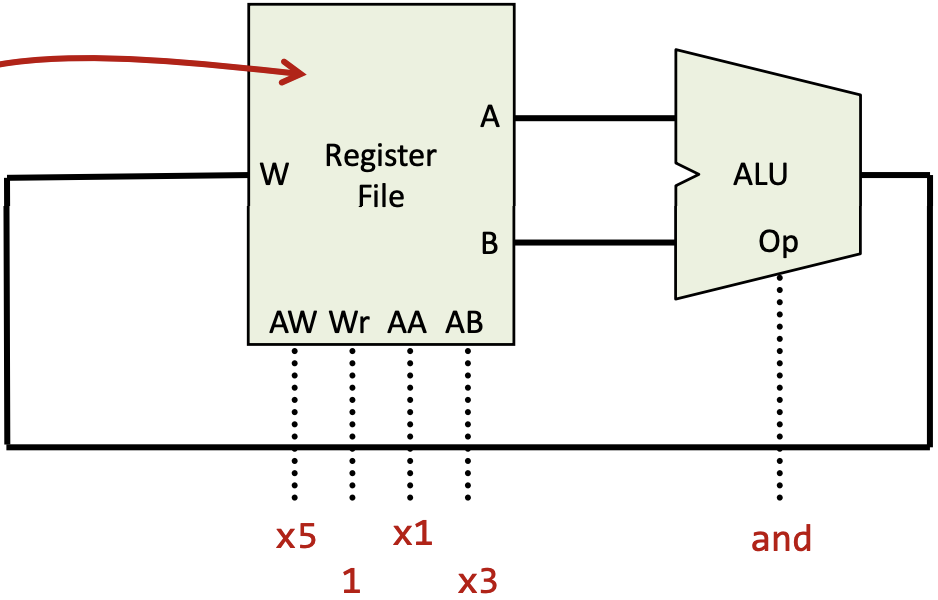
\includegraphics[width=0.45\textwidth]{chapters/chapter1c/images/arith_logic.png}
\end{center}
\subsubsection{Load Instructions}
\begin{center}
    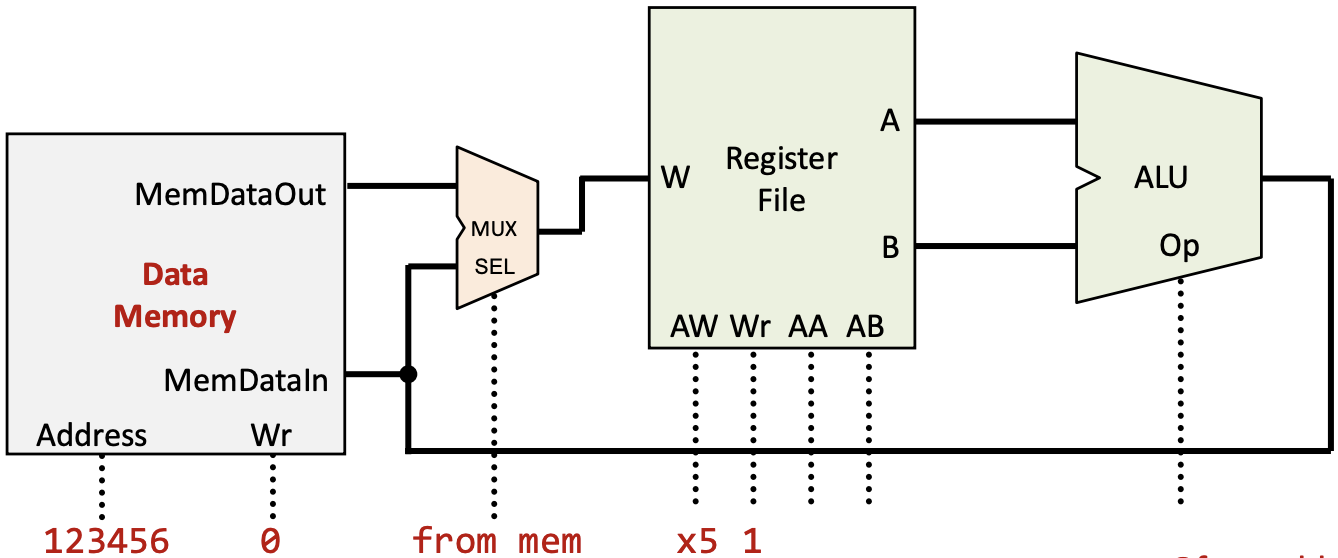
\includegraphics[width=0.45\textwidth]{chapters/chapter1c/images/load.png}
\end{center}
\subsubsection{Load and Store: The RiSC-V Way}
\textit{This instruction would never work for example because the adress is too big to be sent as an immediate value :} \texttt{lw x5, (x7)} \\ \vspace*{5px}
\begin{center}
    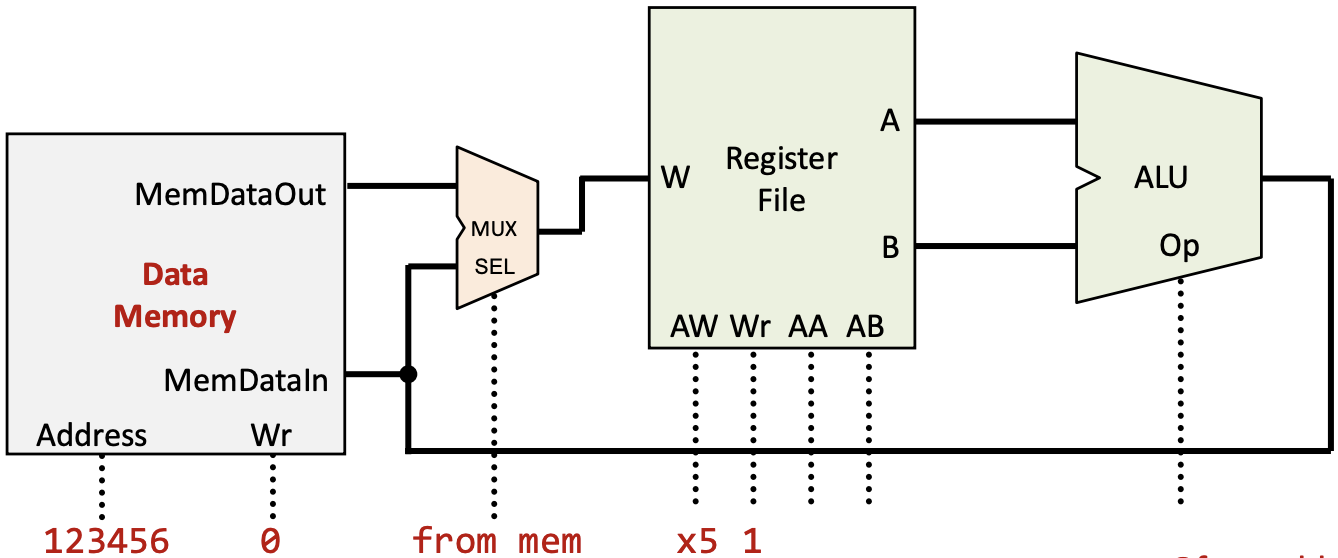
\includegraphics[width=0.45\textwidth]{chapters/chapter1c/images/load.png}
\end{center}
\subsubsection{A Load/Store Architecture}
\textit{A feature of RISC-V is that it's a Load/Store architecture, meaning that the only way to access memory is through load and store instructions. Also, instructions reading and writing in memory do exactly that and nothing else, contrary to more complex instruction set architectures (CISC), where instructions may combine memory access with other operations like arithmetic or logic. This simplicity in RISC-V's instruction set helps with streamlining the pipeline and improving performance efficiency.} \\ \vspace*{5px}

\begin{center}
    \begin{tabular}{|c|c|c|c|c|}
        \hline
        \multicolumn{2}{|c|}{\textbf{Load}} & \textbf{I} & 0x2 & 0x03 \\ 
        \hline
        \texttt{lw} & \texttt{rd,imm(rs1)} & \multicolumn{3}{c|}{\texttt{rd $\leftarrow$ mem[rs1 + sext(imm)]}} \\ 
        \hline
        \multicolumn{2}{|c|}{\textbf{Store}} & \textbf{S} & 0x2 & 0x23 \\ 
        \hline
        \texttt{sw} & \texttt{rs2,imm(rs1)} & \multicolumn{3}{c|}{\texttt{mem[rs1 + sext(imm)] $\leftarrow$ rs2}} \\ 
        \hline
    \end{tabular}
\end{center}

\section{More Addressing Modes? Not in RISC-V!}
\vspace*{-10px}
\begin{center}
\resizebox{1.1\textwidth}{!}{
\begin{tabular}{|l|l|l|}
\hline
\textbf{Addressing Mode}          & \textbf{Instruction}                                      & \textbf{Description}                                                                                   \\ \hline
\textbf{Register}                 & \texttt{add x0, x1, x2}                                   & Adds the value of \texttt{x1} and \texttt{x2}, stores the result in \texttt{x0}.                         \\ \hline
\textbf{Immediate}                & \texttt{add x0, x1, 123}                                  & Adds the value of \texttt{x1} and the immediate constant 123, stores the result in \texttt{x0}.          \\ \hline
\textbf{Direct or Absolute}       & \texttt{add x0, x1, (1234)}                               & Adds the value of \texttt{x1} and the value at memory address 1234, stores the result in \texttt{x0}.    \\ \hline
\textbf{Register Indirect}        & \texttt{add x0, x1, (x2)}                                 & Adds the value of \texttt{x1} and the value in memory at the address held in \texttt{x2}, stores in \texttt{x0}. \\ \hline
\textbf{Displacement or Relative} & \texttt{add x0, x1, 123(x2)}                              & Adds the value of \texttt{x1} and the value in memory at \texttt{x2} plus the displacement 123, stores in \texttt{x0}. \\ \hline
\textbf{Base or Indexed}          & \texttt{add x0, x1, i5(x2)}                               & Adds the value of \texttt{x1} and the value in memory at \texttt{x2} plus index \texttt{i5}, stores in \texttt{x0}. \\ \hline
\textbf{Auto-increment/-decrement} & \texttt{add x0, x1, (x2+)}                               & Adds the value of \texttt{x1} and the value in memory at the address in \texttt{x2}, then increments \texttt{x2}, stores in \texttt{x0}. \\ \hline
\textbf{PC-Relative}              & \texttt{add x0, x1, 123(pc)}                              & Adds the value of \texttt{x1} and the value in memory at \texttt{pc} plus 123, stores in \texttt{x0}.    \\ \hline
\end{tabular}}
\end{center}
    
\textit{Syntax here looks like RISC-V but most of these instructions do not exist in RISC-V.}
\newpage
\subsection{Word Adressed Memory}
\textit{In a word addressed memory, the address is the index of the word in the memory.} \\ 
\textit{The letters inside the word are identified as eg. for Hello World, H:3980, E:3981, L:3982, \dots}.
\begin{center}
    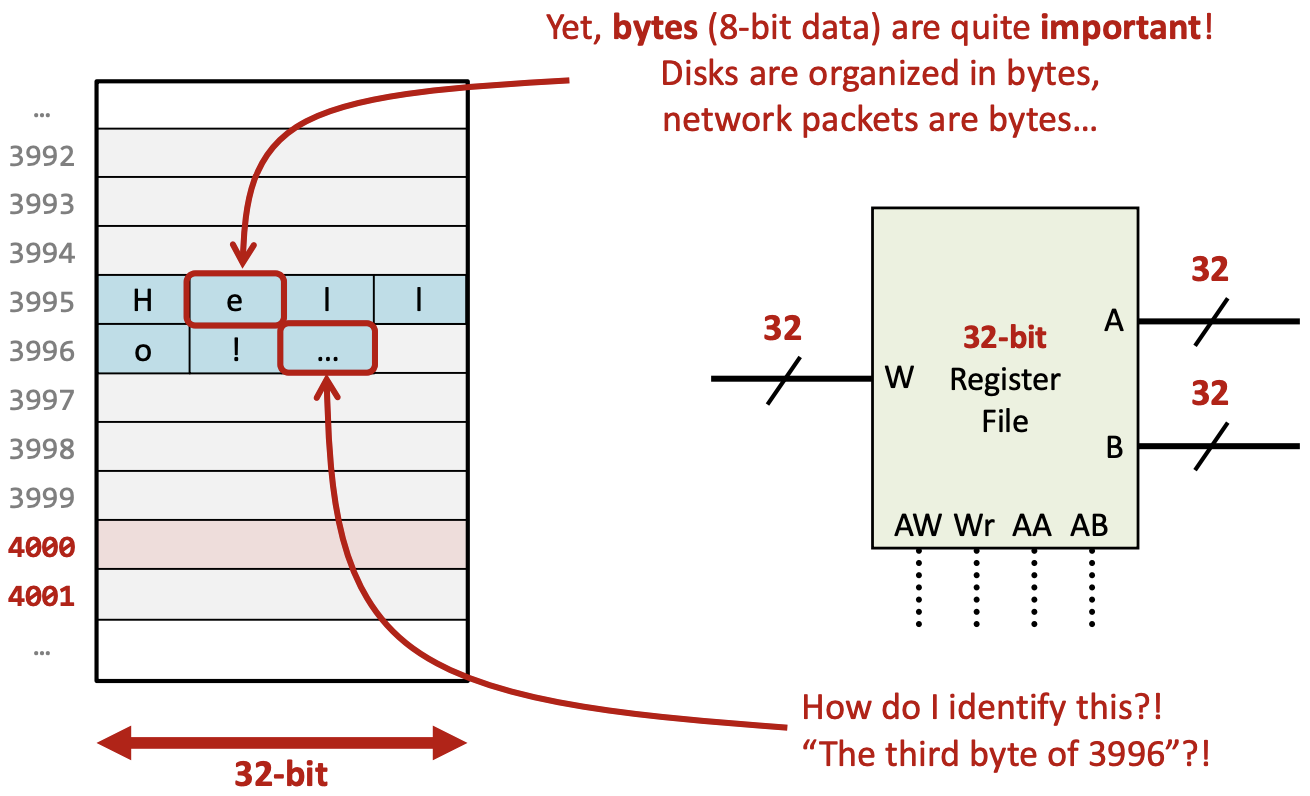
\includegraphics[width=0.45\textwidth]{chapters/chapter1c/images/word_add.png}
\end{center}

\subsection{Loading Words (lw) and Instructions}
\textit{The lw instruction is used to load a word from memory into a register.} \\ 
\textit{The adress of such words would necessarly be a multiple of 4 meaning the two least significant bits must be 0s.(to the ensure the data is word aligned\dots)} \\ 
\begin{center}
    \includegraphics[width=0.45\textwidth]{chapters/chapter1c/images/lw.png}
\end{center}
\subsection{Loading Bytes (lb)}
\textit{The \texttt{lb} (Load Byte) instruction doesn't require alignment because it only loads 1 byte (8 bits), which can be accessed at any memory address, unlike \texttt{lw} which requires word alignment to efficiently load 4 bytes (32 bits).
}\textit{The lb instruction is used to load a byte from memory into a register.} \\ 

\begin{center}
    \includegraphics[width=0.45\textwidth]{chapters/chapter1c/images/lb.png}
\end{center}
\subsection{A Few More Load/Store Instructions}
\textit{Access bytes (and half-words) as if memory were made of bytes}
\begin{center}
    \includegraphics[width=0.45\textwidth]{chapters/chapter1c/images/lb.png}
\end{center}
\subsection{Access as it is more suitable}
\textit{For example storing the "Hello!"zero value in the memory would like this:} \\
\begin{minipage}[htp]{0.45\textwidth}
    \begin{center}
        \includegraphics[width=0.45\textwidth]{chapters/chapter1c/images/hello.png}
    \end{center}
\end{minipage}
\hfill
\vline
\hfill
\begin{minipage}[htp]{ .45\textwidth}
    \begin{center}
        \includegraphics[width=0.3\textwidth]{chapters/chapter1c/images/hello2.png}
    \end{center}
\end{minipage}
\subsubsection{Counting Characters in a String}
\textit{As an example, for counting the number of characters in a string, the load byte instruction would be more suitable as seeing the string as a sequence of bytes makes use of the memory as a sort of array.} \\ \vspace*{5px}

\begin{center}
    \includegraphics[width=0.15\textwidth]{chapters/chapter1c/images/hello2.png}
\end{center}
\begin{center}
    \begin{assembly}
strlen:
    mv t0, a0 # Copy the pointer (a0) into t0 to traverse the string
    li t1, 0 # t1 will hold the length (initialized to 0)
loop:
    lbu t2, 0(t0) # Load byte at address t0 into t2
    beq t2, zero, end # If t2 is 0 (null byte), we are done
    addi t1, t1, 1 # Increment the length counter (t1)
    addi t0, t0, 1 # Point to the next character in the string
j loop # Repeat the loop
end:
    mv a0, t1 # Move the length (t1) into a0 as the return value
    ret # Return to caller
    \end{assembly}
\end{center}

\textit{\texttt{lbu} is used here to ensure that the byte is treated as an unsigned value, which is the correct approach for processing characters in a string.
}
\newpage
In a word addressed memory view, the code would look like such: \\ \vspace*{5px}
\begin{center}
\begin{assembly}
strlen:
    li t1, 0           # t1 will hold the length (initialized to 0)
next_word:
    li t2, 4           # t2 will count the bytes in a loaded word (four)
    lw t3, 0(t0)       # Load four bytes at address t0 into t3
next_byte:
    andi t4, t3, 0xff  # Move the "little-end" in t4
    beq t4, zero, end  # If t4 is 0 (null byte), we are done
    addi t1, t1, 1     # Increment the length counter (t1)
    srli t3, t3, 8     # Prepare the next byte of the word in the "little-end" (t3)
    addi t2, t2, -1    # One byte left in the loaded word
    bnez t2, next_byte # If more bytes in t3, check the next
    addi a0, a0, 4     # Else point to the next word of characters in the string
    j next_word        # Repeat the loop
end:
    mv a0, t1          # Move the length (t1) into a0 as the return value
    ret                # Return to caller
\end{assembly}
\end{center}
\subsection{Loading Bytes (lb)}
\textit{Now, one may wonder in what ordering the bytes are stored in memory.} \\ \vspace*{5px}
\begin{center}
    \includegraphics[width=0.55\textwidth]{chapters/chapter1c/images/lb.png}
\end{center}
\subsubsection{Which Byte Where?}
\textit{Both ordering of bytes are valid the only thing we have to do is stick to one, the most generally used is little-endian as it's the RISCV default and the Intel x86/x64 default.} \\ \vspace*{5px}
\begin{minipage}[htp]{0.45\textwidth}
    \begin{center}
        \textbf{Little Endian} \\ \vspace*{5px}
        \includegraphics[width=0.55\textwidth]{chapters/chapter1c/images/bytes.png}
    \end{center}   
\end{minipage}
\hfill
\vline
\hfill
\begin{minipage}[htp]{0.45\textwidth}
    \begin{center}
        \textbf{Big Endian} \\ \vspace*{5px}
        \includegraphics[width=0.55\textwidth]{chapters/chapter1c/images/bytes2.png}
\end{center}
\end{minipage} \\ \vspace*{5px}
\begin{center}
    \includegraphics[width=0.85\textwidth]{chapters/chapter1c/images/final_endian.png} \\
    \href{https://www.google.com/url?sa=i&url=https%3A%2F%2Fmedium.com%2Fmycsdegree%2Fsockets-in-c-little-and-big-endian-machines-23c9ed484c20&psig=AOvVaw1P8zdPW_G0ioJC2Ka6cOX5&ust=1731236021875000&source=images&cd=vfe&opi=89978449&ved=0CBQQjRxqFwoTCPinlvaKz4kDFQAAAAAdAAAAABAJ}{source}
\end{center}
\textit{Personal Remark : Mnemotechnic - Little Endian = Little End (The ending memory index takes the smallest(starting) data adress), Big Endian = Big End.}
\textit{Or, Little Endian = LSB in smallest index, Big Endian = MSB in smallest index.} % Including chapter0.tex from chapters folder
\chapter{Part I(d) - ISA Arrays and Data Structures - W 2.2}
\section{Arrays}
\textit{In higher level languages, are written like follows :}
\begin{java}
short\[\] myData = \{10407, -16533, -22715, 29796, 18956, \dots\}:
\end{java}
\subsection{Different Ways to Store Arrays}
\begin{center}
    \includegraphics[width=0.45\textwidth]{chapters/chapter1d/images/arrays.png}
\end{center}
\begin{itemize}
\item \textbf{A: Storing Arrays with a Null Terminator}
\begin{itemize}
    \item[-] In this method, the array is stored with each element represented using 16-bit integers.
    \item[-] A null terminator (the value 0) is used at the end of the array to indicate its termination.
    \item[-] This method is common when the array size is unknown in advance, and the null terminator acts as a signal to stop reading the data.
\end{itemize}

\item \textbf{B: Storing Arrays with a Length Prefix}
\begin{itemize}
    \item[-] Here, the first element of the array contains the length of the array, stored as a 16-bit integer (in this case, the length is 9).
    \item[-] The rest of the array is stored in consecutive memory locations, similar to method A.
    \item[-] This method allows the array size to be known before reading all the data, making it more efficient for some use cases.
\end{itemize}

\item \textbf{C: Storing Arrays without a Terminator or Length Prefix}
\begin{itemize}
    \item[-] In this case, the array is stored without a length prefix or a null terminator.
    \item[-] The size of the array must be known externally, either through the code or an external mechanism.
    \item[-] This method is the most compact but requires prior knowledge of the array's size.
\end{itemize}
\end{itemize}

\subsection{Adding Positive Elements}
\textit{Here we'll write the same program for the different ways of storing arrays.} \\
\textit{The program will add all positive elements of an array of signed 16-bit integers. At call time, a0 points to the array, at return time, a0 contains the result.} \\

\textbf{A: Storing Arrays with a Null Terminator}\\
\begin{center}
    \includegraphics[width=0.14\textwidth]{chapters/chapter1d/images/A.png}
\end{center}

\begin{center}
\begin{assembly}
add_pos:li t0, 0         # Initialize t0 to 0
        lh t1, 0(a0)     # Load halfword from memory address a0 into t1
        beqz t1, end     # Branch to 'end' if t1 equals zero
        blez t1, donothing  # Branch to 'donothing' if t1 is less than or equal to zero
        add t0, t0, t1   # Add t1 to t0 (only if t1 is positive)
donothing:               # This block does nothing for negative or zero values
# You can put other operations here if needed
        j add_pos        # Jump back to the beginning of add_pos to check the next value
end:                     # Label 'end' for the program termination
\end{assembly}
\end{center}
\textbf{B: Storing Arrays with a Length Prefix} \\
\begin{center}
    \includegraphics[width=0.14\textwidth]{chapters/chapter1d/images/B.png}
\end{center}

\begin{center}
\begin{assembly}
add_pos_b:  
    lh t2, 0(a0)        # Load the length of the array into t2
    addi a0, a0, 2      # Move to the first element of the array (skip the length prefix)
    li t0, 0            # Initialize t0 to 0 for storing the sum
loop_b:    
    beqz t2, end_b      # If the length (t2) is zero, branch to 'end_b'
    lh t1, 0(a0)        # Load the current array element into t1
    blez t1, skip_b     # If t1 is less than or equal to zero, skip the addition
    add t0, t0, t1      # Add t1 to t0 (only if t1 is positive)
skip_b:    
    addi a0, a0, 2      # Move to the next element in the array
    addi t2, t2, -1     # Decrease the length counter
    j loop_b            # Jump back to loop_b
end_b:                  # End label
\end{assembly}
\end{center}
\textbf{C: Storing Arrays without a Terminator or Length Prefix} \\
\begin{center}
    \includegraphics[width=0.14\textwidth]{chapters/chapter1d/images/C.png}
\end{center}

\begin{center}
\begin{assembly}
add_pos_c:  
    li t0, 0         # Initialize t0 to 0 for storing the sum
loop_c:     
    beqz t2, end_c   # If the array size (t2) is zero, branch to 'end_c'
    lh t1, 0(a0)     # Load the current array element into t1
    blez t1, skip_c  # If t1 is less than or equal to zero, skip the addition
    add t0, t0, t1   # Add t1 to t0 (only if t1 is positive)
skip_c:    
    addi a0, a0, 2   # Move to the next element in the array
    addi t2, t2, -1  # Decrease the array size counter
    j loop_c         # Jump back to loop_c
end_c:               # End label
\end{assembly}
\end{center}

\subsection{Pointer to Memory vs Index in Array}
\textit{Now we're wodnering which one of these two ways of accessing the array is better.} \\
\textbf{Obviously the less instructions the better (not always true actually but well),\\ Pointer to Memory.} \\
\begin{minipage}[htpb]{0.45\textwidth}
\begin{assembly}
add_positive:
    li t0, 0
    mv t1, a1
next_short:
    beq t1, zero, end
    lh t2, 0(a0)
    bltz t2, negative
    add t0, t0, t2
negative:
    addi a0, a0, 2
    addi t1, t1, -1
    j next_short
end:
    mv a0, t0
ret
\end{assembly}
\end{minipage}
\hfill
\vline
\hfill
\begin{minipage}[htp]{0.45\textwidth}
\begin{assembly}
add_positive:
    li t0, 0
    li t1, 0
next_index:
    bge t1, a1, end
    slli t2, t1, 1
    add t2, a0, t2
    lh t3, 0(t2)
    bltz t3, negative
    add t0, t0, t3
negative:
    addi t1, t1, 1
    j next_index
end:
    mv a0, t0
ret
\end{assembly}
\end{minipage}
\newpage
\subsubsection{In C}
\textit{Writing this in C for better understanding. Again, which one is better?} \\
\vspace*{5px}
\textbf{Obviously the less instructions the better (again not always true but ah), Index in array} \\
\begin{minipage}[htp]{0.45\textwidth}
\textbf{Pointer to memory} \\
\begin{cc}
short sum = 0;
short *ptr = myData;
short *end = myData + N;
while (ptr < end) {
    if (*ptr > 0) {
    sum += *ptr;
}
    ptr++;
}
\end{cc}
\end{minipage}
\hfill
\vline
\hfill
\begin{minipage}[htp]{0.45\textwidth}
\textbf{Index in array} \\
\begin{cc}
short sum = 0;
int i;
for (i = 0; i < N; i++) {
    if (myData[i] > 0) {
    sum += myData[i];
}
}
\end{cc}
\end{minipage}

\subsubsection{We need a good compiler}
\textit{Seeing this, the idea would be to have a sufficiently good \textbf{compiler} (check I.4.3.2 if needed) such that we write our C code in Index in array, and we get Pointer to memory code in assembly. Thus writing better code but also getting better performance.} \\
\textbf{Another type of collection we could've used to store the data is a \textit{Linked List}.} \\
\vspace*{5px}
\begin{minipage}[htp]{0.45\textwidth}   
    \textit{Linked lists are useful for efficiently inserting and deleting elements, especially in the middle of the list.} \\
    \vspace*{5px}
    \textit{Each 32-bit element in a linked list contains 16 bits for the value and 16 bits for the address of the next element, enabling efficient insertions but slower sequential access compared to arrays.}
\end{minipage}
\hfill
\vline
\hfill
\begin{minipage}[htp]{0.45\textwidth}
\begin{center}
    \includegraphics[width=0.95\textwidth]{chapters/chapter1d/images/linked_list.png}
\end{center}
\end{minipage} % Including chapter0.tex from chapters folder

\chapter{Part I(e) - ISA Arithmetic - W 3.1}
\section{Notation}
Before we start, let's define some notation:
\begin{itemize}
    \item[-] \textbf{Number representation (with a fixed number of digits/bits):}
    \[
    A = A^{(n)} = A^{(m)}
    \]
    
    \item[-] \textbf{Number in binary or decimal:}
    \[
    A = A_{10} = A_{2} = A_{2c}
    \]
    \textit{With $A_{2c}$ being the 2's complement representation.} \\
    \textit{And $A_{2}$ being the binary representation.}
    \item[-] \textbf{Individual digits or bits:}
    \[
    a_{n-1}, a_{n-2}, \dots, a_2, a_1, a_0
    \]
    
    \item[-] \textbf{Digit string representation:}
    \[
    \langle a_{n-1} a_{n-2} \dots a_2 a_1 a_0 \rangle
    \]
\end{itemize}

\section{Numbers}

Numbers in computing can be represented in different forms, each with specific use cases. \\
\vspace*{5px}
\textbf{Integers} can be either signed or unsigned, representing positive and negative values, or only non-negative values. Examples include:
\[
0, 1, 2, 3, 4294967295, -2147483648
\]

\textbf{Fixed-point} numbers are essentially integers with an implicit scaling factor (e.g., \(10^k\) or \(2^k\)) to handle fractional values. Common in applications like signal processing. Examples include:
\[
0.12, 3.14, 1073741823.75
\]

\textbf{Floating-point} numbers represent a wide range of values using a base and exponent, providing flexibility in precision. Examples include:
\[
3.14E3, -2.5E1, 1.0E0, 4.2E-2, -1.5E-3
\]

\subsection{Unsigned Integers}
Unsigned integers are:
\begin{itemize}
    \item[-] \textit{Weighted}: Each digit has a positional value.
    \item[-] \textit{Nonredundant}: Every number has a unique representation.
    \item[-] \textit{Based on a fixed-radix system}: Typically radix-10 (decimal) or radix-2 (binary).
    \item[-] \textit{Canonical}: Follows a standard form for representation.
\end{itemize}

\textbf{Definition:}
\[
A = \langle a_{n-1} a_{n-2} \dots a_2 a_1 a_0 \rangle = \sum_{i=0}^{n-1} a_i R^i
\]
where \(A\) is the unsigned integer, \(a_i\) are the digits, and \(R\) is the radix.

\subsection{Signed Integers}
We may distinguish between three methods for representing signed integers:
\begin{itemize}
    \item \textbf{Sign-and-Magnitude (SM)}: Uses the most significant bit (MSB) to represent the sign (0 for positive, 1 for negative), with the remaining bits representing the magnitude. This method has the drawback of two zeros (+0 and -0) (Redundant).
    \item \textbf{Two's Complement}(Specific True-and-Complement): The most common way to represent signed integers. It avoids the two-zero problem and simplifies arithmetic operations. Negative numbers are represented by flipping the bits and adding 1.
    \item \textbf{Biased Representation}: Primarily used in floating-point numbers, especially for the exponent part. A fixed bias is added to the actual value to avoid negative exponents. It's rarely used for integers but is another method for handling signed numbers.
\end{itemize}
\subsubsection{Sign and Magnitude}
In the sign-and-magnitude representation, the most significant bit (MSB) is used to represent the sign of the number. The remaining bits represent the magnitude. \\
\vspace*{7px}
\textbf{Definition} \\
\vspace*{3px}
\[
A = \langle s a_{n-2} a_{n-3} \dots a_2 a_1 a_0 \rangle = (-1)^s \cdot \sum_{i=0}^{n-1} a_i R^i
\]
where \(A\) is the signed integer, \(s\) the most significant bit of \(A\) representing the sign of the number, \(a_i\) the digits, and \(R\) the radix. \\
\vspace*{7px}
\textbf{Example (Signed 4-bit integer):} \\
\vspace*{3px}

Consider the 4-bit signed binary number \(1011_2\). In this case: \\
\begin{itemize}
    \item[1.] The MSB \(s = 1\), indicating the number is negative.
    \item[2.] The magnitude bits are \(011_2 = 3_{10}\).
    \item[3.] Therefore, the value of the number is \(-3\).
\end{itemize}

Thus, \(1011_2\) represents \(-3_{10}\) in sign-and-magnitude representation. \\
\vspace*{7px}

\subsection{Radix's Complement}
Radix's complement is a method used to represent signed numbers in different number systems. \\
It is a special form of \textit{true-and-complement} where the complement $C = R^n$, with $R$ being the radix (base) and $n$ the number of digits. \\
\vspace*{5px}
\begin{center}
    \includegraphics[width=0.65\textwidth]{chapters/chapter1e/images/twoscomplement.png}
\end{center}
\textbf{Definition} \\
\vspace*{2px}
A number $A$ in radix's complement is represented as:
\[
A = \langle a_{n-1}a_{n-2}\dots a_1a_0 \rangle = -a_{n-1}R^{n-1} + \sum_{i=0}^{n-2} a_i R^i
\]
where $a_{n-1}$ is the most significant bit, which also indicates the sign (negative for $a_{n-1} = 1$). \\
\vspace*{5px}
For binary numbers, radix’s complement is known as \textbf{two's complement}, which is the most commonly used method for representing signed numbers in digital systems. \\
\vspace*{5px}
\textbf{Binary (2's Complement) Representation} \\
\vspace*{2px}
Two's complement uses base $R = 2$ and has a fixed word length $n$. \\
Here is an example for an 8-bit number system:



\begin{center}
\begin{tabular}{|c|c|c|}
\hline
\textbf{Binary} & \textbf{Decimal} & \textbf{Range} \\
\hline
00000000 & 0   & \multirow{2}{*}{Positive range} \\
01111111 & 127 & \\
\hline
10000000 & -128 & \multirow{2}{*}{Negative range} \\
11111111 & -1   & \\
\hline
\end{tabular}
\end{center}

The two's complement system enables representation of both positive and negative numbers within a fixed bit length. \\
\vspace*{5px}
\textbf{Decimal (10's Complement) Representation} \\
\vspace*{2px}
In a decimal system with radix $R = 10$,\\
We use 10's complement to represent signed numbers. For instance: \\
\[
5,678_{(5)}^{10c} = 05,678_{10c} = +5,678_{10}
\]
This is a positive number representation in 10's complement. For a negative number: \\

\[
9,999,999_{(7)}^{10c} = -1_{10}
\]
Here, $9,999,999$ in 7 digits represents $-1$ in decimal form. \\
\vspace*{5px}
\textbf{Examples of Binary (2's Complement)} \\
\vspace*{2px}
Below are several examples of numbers in binary (2's complement) and their corresponding decimal values: \\
This is a positive binary number. \\
\[
0100,1101,0010_{(12)}^{2c} = 100,1101,0010_2 = +1,234_{10}
\]

This is a negative binary number in 8-bit representation.\\
\[
1111,1111_{(8)}^{2c} = -1_{10}
\]

This is a negative binary number in 12-bit representation.\\
\[
1011,0000,1110_{(12)}^{2c} = -1,234_{10}
\]
\vspace*{5px}

\subsection{Two's Complement Subtraction}

Consider the binary subtraction using the standard paper-and-pencil method:

\[
\begin{array}{cccccccccc}
\text{Borrow:} & -1 & -1 & -1 & & & & -1 & & \\
& 0 & 0 & 0 & 0 & 1 & 0 & 1 & 0 & \quad (10_{10}) \\
- & 0 & 0 & 0 & 1 & 0 & 0 & 0 & 1 & \quad (17_{10}) \\
\hline
  & 1 & 1 & 1 & 1 & 1 & 0 & 0 & 1 \\
\end{array}
\]


Since we had to borrow beyond the most significant bit, the result is negative. The binary result is:
\[
-1\ 1\ 1\ 1\ 1\ 0\ 0\ 1_2
\]

To find its decimal value:
\begin{center}
    $-2^7 + 2^6 + 2^5 + 2^4 + 2^3 + 2^0 = -128 + 64 + 32 + 16 + 8 + 1 =-7$ \\
    and \\
    $
    10_{10} - 17_{10} = -7_{10}
    $
\end{center}


\subsection{Addition Is Unchanged from Unsigned}

In arithmetic operations, addition remains consistent whether using signed or unsigned numbers. The following instructions are available for basic arithmetic operations:
\begin{center}
    \includegraphics[width=0.75\textwidth]{chapters/chapter1e/images/addition.png}
\end{center}
\begin{itemize}
    \item[-] \texttt{add rd, rs1, rs2}: Adds the values in \texttt{rs1} and \texttt{rs2}, and stores the result in \texttt{rd}.
    \item[-] \texttt{addi rd, rs1, imm}: Adds the value in \texttt{rs1} with the sign-extended immediate value \texttt{imm}, and stores the result in \texttt{rd}.
    \item[-] \texttt{sub rd, rs1, rs2}: Subtracts the value in \texttt{rs2} from \texttt{rs1}, and stores the result in \texttt{rd}.
\end{itemize}
 
Note that older architectures (e.g., MIPS) had distinct instructions for signed (\texttt{add}) and unsigned (\texttt{addu}) addition. However, this distinction is unnecessary as the hardware handles both identically. \\
\vspace*{5px}
Sign-and-magnitude addition presents unique challenges, making \textbf{two's complement} the standard for signed integers in modern architectures.

\subsection{Sign Extension}

In digital systems, sign extension is a technique used to increase the bit width of a binary number while preserving its value and sign. It is commonly used when converting a number from a smaller to a larger bit width in a way that maintains its original meaning, whether it's unsigned or in two’s complement format.


\subsubsection{Example: 4-bit to 8-bit Conversion}
Consider the 4-bit two’s complement number \( 1110_2 \), which represents \( -2_{10} \).\\
When extending this number to 8 bits, we replicate the MSB (which is 1 in this case) to fill the additional bits, as shown below: \\
\[
5_{10} = 0101_2 \quad \text{(4 bits)} \to \quad 00000101_2 \quad \text{(8 bits)}.
\] \\
while 
\[
-2_{10} = 1110_2 \quad \text{(4 bits)} \quad \to \quad 11111110_2 \quad \text{(8 bits)}.
\]

This ensures that the number remains \( -2_{10} \) even after increasing the bit width. \\
\vspace*{5px}


\textit{\textbf{Truncation} is allowed when reducing bit width, but only if the truncated bits are redundant (i.e., copies of the sign bit). For example, going from 8 bits back to 4 bits would result in \( 1110_2 \), preserving the value \( -2_{10} \).
}

\subsection{Signed and Unsigned Instructions}
In RISC-V, instructions differentiate between signed (s) and unsigned (u) operations:

\begin{center}
    \includegraphics[width=0.75\textwidth]{chapters/chapter1e/images/ref_card.png}
\end{center}
\begin{itemize}
    \item \textbf{Shift:} \texttt{sra}, \texttt{srai} (s) vs. \texttt{srl}, \texttt{srli} (u). 
    \begin{itemize}
        \item Signed shifts preserve the sign bit, while unsigned shifts insert zeroes.
    \end{itemize}
    
    \item \textbf{Compare:} \texttt{slt}, \texttt{slti} (s) vs. \texttt{sltu}, \texttt{sltiu} (u). 
    \begin{itemize}
        \item Signed comparisons use two's complement, unsigned comparisons ignore sign.
    \end{itemize}
    
    \item \textbf{Branch:} \texttt{blt}, \texttt{bge} (s) vs. \texttt{bltu}, \texttt{bgeu} (u). 
    \begin{itemize}
        \item Signed branches use two's complement; unsigned branches do not consider sign.
    \end{itemize}
    
    \item \textbf{Load:} \texttt{lb}, \texttt{lh} (s) vs. \texttt{lbu}, \texttt{lhu} (u). 
    \begin{itemize}
        \item Signed loads extend the sign bit, while unsigned loads extend with zeroes.
    \end{itemize}
\end{itemize}


\section{Overflow}

Overflow occurs when the result of an arithmetic operation exceeds the range of values that can be represented with a fixed number of bits. This can happen in both unsigned and signed arithmetic, though the detection method differs. In general, overflow results in an incorrect outcome that needs to be detected and handled.

\subsection{Overflow in 2's Complement}

In 2's complement arithmetic, overflow occurs when the result of an addition or subtraction operation falls outside the representable range for the number of bits. For an \(n\)-bit 2's complement system, the representable range is \(-2^{n-1}\) to \(2^{n-1} - 1\).

Overflow is detected by examining the carry into and out of the most significant bit (MSB). Specifically, overflow occurs if:

\[
\text{Overflow} = \text{Cout}_{n-1} \oplus \text{Cout}_n
\]

Where:
\begin{itemize}
    \item[-] \(\text{Cout}_{n-1}\) is the carry into the MSB.
    \item[-] \(\text{Cout}_n\) is the carry out of the MSB.
\end{itemize}

An overflow occurs when these two carry bits differ. This is because the sign of the result is incorrect if there is a mismatch, leading to an incorrect outcome.

\begin{center}
    \includegraphics[width=0.65\textwidth]{chapters/chapter1e/images/sum.png}
\end{center}

For example, if two large positive numbers are added and result in a negative value (or two negative numbers added result in a positive value), this indicates an overflow in 2's complement addition.

\subsection{Overflow in Software}

In many architectures, detecting overflow during arithmetic operations is a critical aspect of software implementation. Overflow occurs when the result of an addition or subtraction exceeds the capacity of the register used to store it. Detection methods vary depending on the type of architecture:

\begin{itemize}
    \item \textbf{Traditional architectures (e.g., x86):} These systems provide a \textit{carry bit} in a special register, known as a flag, that is set when an overflow occurs. Thus, overflow detection operates similarly to hardware-based overflow detection.
    
    \item \textbf{Modern architectures (e.g., RISC-V):} These architectures typically provide only the result of the addition or subtraction without a carry bit. Overflow detection must be handled in software, based on analyzing the sign and magnitude of the result.
\end{itemize}

\begin{center}
    \includegraphics[width=0.65\textwidth]{chapters/chapter1e/images/overflow.png}
\end{center}
Overflow detection can be based on the following observations:
\begin{itemize}
    \item[-] \textbf{Addition of opposite sign numbers:} The magnitude of the result decreases, making overflow impossible.
    \item[-] \textbf{Addition of same sign numbers:} Overflow is possible if the result exceeds the range representable by the register, leading to an incorrect sign in the result.
\end{itemize}
\subsection{Detect Addition Overflow in Software}
\begin{itemize}
    \item[-] Add two 32-bit signed integers and detect overflow
    \begin{itemize}
        \item At call time, a0 and a1 contain the two integers
        \item On return, a0 contains the result and a1 must be nonzero in case of overflow
    \end{itemize}
\end{itemize}


\subsection{Detect Addition Overflow in Software}
\begin{itemize}
    \item[-] Add two 32-bit signed integers and detect overflow
    \begin{itemize}
        \item At call time, \texttt{a0} and \texttt{a1} contain the two integers.
        \item On return, \texttt{a0} contains the result and \texttt{a1} must be nonzero in case of overflow.
    \end{itemize}
\end{itemize}

\begin{assembly}
srai a2, a0, 31       # a2 = sign of a0 (0 or -1)
srai a3, a1, 31       # a3 = sign of a1 (0 or -1)
xor  a4, a2, a3       # a4 = 0 if signs are same, -1 if different
add  a0, a0, a1       # compute sum in a0
srai a5, a0, 31       # a5 = sign of sum (0 or -1)
xor  a6, a2, a5       # a6 = 0 if sign of sum same as a0, -1 if different
and  a1, a4, a6       # a1 = -1 if overflow occurred, else 0
srli a1, a1, 31       # a1 = 1 if overflow occurred, else 0
\end{assembly}

\section{A Strange but Useful Property}
\textit{Personal Remark: don't mistake A and $\overline{A}$ as sets of elements which might confuse you. They are binary numbers.} \\
In binary arithmetic, there is a particularly useful property that can be expressed as follows:

\[
A + \overline{A} = -1
\]
or equivalently,
\[
-A = \overline{A} + 1
\]

\textbf{Proof:} Consider a binary number $A = a_{n-1}2^{n-1} + \sum_{i=0}^{n-2} a_i 2^i$, where $a_i \in \{0,1\}$ represents the binary digits of $A$. The complement of $A$, denoted $\overline{A}$, is given by replacing each $a_i$ with its complement $\overline{a_i}$.

\[
A + \overline{A} = \left( -a_{n-1}2^{n-1} + \sum_{i=0}^{n-2} a_i 2^i \right) + \left( -\overline{a_{n-1}} 2^{n-1} + \sum_{i=0}^{n-2} \overline{a_i} 2^i \right)
\]
\[
= -(a_{n-1} + \overline{a_{n-1}}) \cdot 2^{n-1} + \sum_{i=0}^{n-2} (a_i + \overline{a_i}) \cdot 2^i
\]
\[
= -2^{n-1} + \sum_{i=0}^{n-2} 2^i = -1
\]
\textit{Where $\overline{A}$ is the two's complement of $A$.} \\
\textbf{Intuition:} For each binary digit, adding $a_i$ and its complement $\overline{a_i}$ results in $1$. Therefore, $A + \overline{A}$ consists entirely of $1$s, representing $-1$ in two's complement.
\subsection{Two's Complement Subtractor}
Using the property of two's complement, we can create a subtractor circuit. The subtractor is implemented using an adder, where the number to be subtracted is inverted and incremented by 1.

\begin{itemize}
    \item[-] \textbf{Step 1: Inversion of Subtrahend (B)}\\
    The subtrahend $B$ is inverted using NOT gates, as shown in the diagram. This converts $B$ into its one's complement.
    
    \item[-] \textbf{Step 2: Addition of A and Inverted B}\\
    The full adders (FA) add each bit of the minuend $A$ to the inverted bits of $B$. The full adders also handle any carry-over from the previous addition.

    \item[-] \textbf{Step 3: Add 1 (Two's Complement)}\\
    To complete the two's complement operation, a carry-in of 1 is added to the least significant bit (LSB), which effectively adds 1 to the inverted $B$.

    \item[-] \textbf{Output:}\\
    The sum outputs $S$ ($s_0, s_1, s_2, ...$) represent the result of the subtraction $A - B$, while the final carry-out can be used to detect overflow.
\end{itemize}

\begin{center}
    \includegraphics[width=0.65\textwidth]{chapters/chapter1e/images/substractor.png}
\end{center}

\subsection{Two's Complement Add/Subtract Unit}
This circuit performs both addition and subtraction using two's complement arithmetic. The operation is selected based on the control input signal for subtraction. The unit consists of several key components:

\begin{itemize}
    \item[-] \textbf{Input Inversion:} Each bit of the subtrahend $B$ is passed through a XOR gate controlled by the `subtract` signal. When the `subtract` signal is high (logic 1), the bits of $B$ are inverted to form the two's complement of $B$, effectively switching the operation to subtraction.
    
    \item[-] \textbf{Addition:} The ripple-carry adder, represented by the ADDER block, performs binary addition of the bits from $A$ and $B$. The carry-in ($Cin$) to the least significant bit is used to add 1 when performing subtraction, completing the two's complement process.
    
    \item[-] \textbf{Overflow Detection:} The overflow generator block detects if the result of the addition/subtraction operation has exceeded the range representable by the fixed number of bits. The `overflow` output is asserted in such cases.
    
    \item[-] \textbf{Output:} The result of the operation is provided as the sum output ($S$), representing either the sum $A + B$ or the result of $A - B$, depending on the control signal.
\end{itemize}

\begin{center}
    \includegraphics[width=0.65\textwidth]{chapters/chapter1e/images/adder_substractor.png}
\end{center}


\section{Bounds Check Optimization}
\textit{Very, very, very useful.}
When working with signed integers (e.g., array indices), a common task is to ensure that the index remains within a valid range, typically \(0 \leq t0 < N\), where \(N\) is some predefined boundary. \\
This can be achieved efficiently using a single branch check that combines both lower and upper bound constraints. \\
\vspace*{7px}
\textbf{Single Branch Bound Check} \\
\vspace*{3px}
The instruction \texttt{bgeu} (branch if greater than or equal, unsigned) can perform two checks at once:
\[
\texttt{bgeu}\ t0, t1, \texttt{out\_of\_bound}
\]
Here, \(t0\) is the signed number to be checked, and \(t1 = N\) is the boundary. \\
\vspace*{7px}
\textbf{Explanation} \\
\begin{itemize}
    \item[-] If \(t0 \geq 0\), the behavior of \texttt{bgeu} mimics that of \texttt{bge} (branch if greater than or equal) for signed integers, thus effectively performing an upper bound check.
    \item[-] If \(t0 < 0\), since the comparison is unsigned, \(t0\) will appear as a very large positive value, hence automatically triggering the out-of-bound case.
\end{itemize}

This approach efficiently checks both the lower and upper bounds in one instruction, streamlining the bounds checking process.

\section{Floating Point Representation}

Floating point numbers are widely used in computing to represent real numbers in a way that supports a wide dynamic range. \\
\vspace*{5px}
They are composed of a \textit{significand} (or \textit{mantissa}) and an \textit{exponent} of the base. This representation allows for the approximation of very large and very small values, similar to the way scientific notation is used in everyday practices.\\
\vspace*{5px}
\textbf{Such as}
\begin{align*}
    0.18 \ \mu\text{m} & \quad \rightarrow \quad 0.18 \cdot 10^{-6} \ \text{m} \quad \rightarrow \quad 1.8 \cdot 10^{-7} \ \text{m} \\
    75 \ \text{km} & \quad \rightarrow \quad 75 \cdot 10^{3} \ \text{m} \quad \rightarrow \quad 7.5 \cdot 10^{4} \ \text{m}
\end{align*}


In floating point representation, a number \( X \) is expressed as:
\[
X = (-1)^s \cdot \left(\sum_{i=0}^{n-1} a_i \cdot 2^i \right) \cdot 2^{\left( - e_{m-1} 2^{m-1} + \sum_{j=0}^{m-2} e_j 2^j \right)}
\]
where:
\begin{itemize}
    \item[-] \( s \) is the sign bit,
    \item[-] \( a_i \) represents the bits of the significand (in sign-and-magnitude form),
    \item[-] \( e_j \) represents the bits of the exponent (in 2's complement form).
\end{itemize}

\subsubsection{Properties of Floating Point Numbers}
\begin{itemize}
    \item[-] \textbf{Large dynamic range}, but \textit{variable accuracy}.
    \item[-] Numbers are \textbf{redundant} unless \textit{normalized}.
    \item[-] Floating point operations are \textbf{not associative}, unlike real numbers.
    \item[-] Exponents are typically stored in a \textbf{biased signed representation}, making zero easier to represent and simplifying comparisons in hardware.
    \item[-] The \textbf{mantissa} (significand) is usually normalized such that \(1 \leq m < 2\), with a \textit{hidden bit} to store the leading 1.
\end{itemize}

\subsubsection{Standardization and Hardware Support}
Floating point representation is standardized by the IEEE 754 standard, which is widely adopted in modern computing systems:
\begin{itemize}
    \item[-] \textbf{x86/x64} architectures have supported floating point operations through SSE/AVX extensions since 1999.
    \item[-] \textbf{RISC-V} also includes support for floating point through ISA extensions.
\end{itemize}

\subsubsection{Example: Decimal to IEEE 754 Simple Precision (32 Bits) Conversion}
Convert \( -7.75 \) to IEEE 754 single-precision:

\begin{minipage}[t]{0.45\textwidth}
\vspace*{5px}
\textbf{Step 1: Sign Bit (1 Bit)}\\  
\vspace*{5px}
\( s = 1 \) (negative number). \\
\vspace*{5px} 
\textbf{Step 2: Binary Conversion}\\  
\vspace*{5px}
\( 7_{10} = 111_2 \), \( 0.75_{10} = 0.11_2 \), so \( 7.75_{10} = 111.11_2 \). \\
\textbf{Step 3: Normalize}\\
\vspace*{5px}  
\( 111.11_2 = 1.1111_2 \times 2^2 \). \\
\vspace*{5px}
\textbf{Step 4: Exponent (8 Bits)}\\
\vspace*{5px}  
\( E = 2 + 127 = 129 \), \( 129_{10} = 10000001_2 \).
\end{minipage}
\hfill
\vline
\hfill
\begin{minipage}[t]{0.45\textwidth}

\textbf{Step 5: Mantissa (23 Bits)}\\
\vspace*{3px}  
\begin{justify}
    Take the fractional part after the leading 1 and pad with zeros to make 23 bits:
\end{justify} 
\( 1111 \ 0000 \ 0000 \ 0000 \ 0000 \ 000 \) \\
(fractional part after the leading 1). \\
\vspace*{3px}
\textbf{Step 6: IEEE 754 Representation}\\
\vspace*{3px}  
\[
\boxed{
  \underbrace{1}_{\text{Sign bit}} \ 
  \underbrace{10000001}_{\text{Exponent bits}} \ 
  \underbrace{1111 \ 0000 \ 0000 \ 0000 \ 0000 \ 000}_{\text{Mantissa}}
}
\]
\end{minipage}

\subsection{Sign-and-Magnitude Addition}

In this exercise, we aim to write a function in RISC-V assembler to sum two 32-bit signed numbers represented in sign-and-magnitude (S\&M) format. The result should also be produced in the sign-and-magnitude format.

\begin{itemize}
    \item[-] The two operands are stored in registers \texttt{a0} and \texttt{a1} on entry.
    \item[-] The result should be placed in register \texttt{a0}.
    \item[-] Overflow cases should be ignored.
\end{itemize}

\begin{assembly}
# Load the operands from a0 and a1
# Mask the sign bits
andi t0, a0, 0x7FFFFFFF   # Extract magnitude of a0
andi t1, a1, 0x7FFFFFFF   # Extract magnitude of a1

# Extract the signs (MSB) of both operands
srai t2, a0, 31           # Sign of a0
srai t3, a1, 31           # Sign of a1

# Compare the signs
beq t2, t3, same_sign     # If signs are equal, sum the magnitudes
sub t0, t0, t1            # If signs differ, subtract the magnitudes
j check_result            # Jump to check the result

same_sign:
    add t0, t0, t1            # Add magnitudes if signs are the same

check_result:
    # Restore the sign in the result
    slli t0, t2, 31           # Shift the sign bit into position
    or a0, t0, t1             # Combine sign and magnitude into a0
\end{assembly}














 % Including chapter0.tex from chapters folder

\end{document}

